% =================================================================================
% Hier ausw�hlen, ob TUD-Design oder nicht
% =================================================================================
\newif\ifTUDdesign
\TUDdesigntrue					% TUD-Design
%\TUDdesignfalse				% F�r Rechner ohne installierte TUDdesign-Pakete
% =================================================================================


% =================================================================================
% Hier Daten f�r studentische Arbeit eingeben
% =================================================================================
\newcommand{\SADATyp}{Praktikumsbericht}
\newcommand{\SADATitel}{Praktikumsbericht\\}
\newcommand{\SADAStadt}{Stuttgart}
\newcommand{\SADAUnternehmen}{Vector Informatik GmbH}
\newcommand{\SADAAutor}{Samir Alexis Revelo Cordoba}
\newcommand{\SADABetreuer}{Dipl.-Ing. Hartmut H�rner}
\newcommand{\SADABetreuerII}{Dipl.-Ing. Markus Schwarz}
\newcommand{\SADABegin}{01. April 2016}
\newcommand{\SADAAbgabe}{31. September 2016}
\newcommand{\SADASeminar}{27. November 2013}


% =================================================================================


% =================================================================================
% Auswahl des IAT-Fachgebiets (rtm / rtp)
% =================================================================================
\newif\ifrtm
%\rtmtrue	% rtm
\rtmfalse	% rtp

% =================================================================================


% =================================================================================
% Erkl�rung, dass die Arbeit ohne Hilfe Dritter etc. erstellt wurde
% =================================================================================
\def\SADAVarianteErklaerung{ETIT}		% FB 18, Elektrotechnik
%\def\SADAVarianteErklaerung{MBDA}		% FB 16, Maschinenbau, Diplomarbeit
%\def\SADAVarianteErklaerung{MBSA}		% FB 16, Maschinenbau, Studienarbeit
% =================================================================================


% =================================================================================
% Ausnahmen von der automatischen Silbentrennung
% =================================================================================
\hyphenation{Aktu-ali-sie-rung Screen-shots Pa-rallel-ro-bo-ter Zu-stands-raum-mo-del-le nach-voll-zieh-bar Pro-jekt-se-mi-nar}
% =================================================================================


% =================================================================================
% Hier NIICHTS �ndern!
% =================================================================================
\ifTUDdesign
	\documentclass[11pt, twoside, colorback, accentcolor=tud9c, nopartpage, bigchapter, fleqn, ngerman, longdoc]{tudreport}
		
\else
	\documentclass[11pt, a4paper, twoside, fleqn, ngerman]{scrreprt}
  % F�r Entwurf auf Rechnern ohne installierte TUDdesign-Pakete	
	\usepackage{exscale}	% Korrektur math-Zeichen
	\usepackage{eurosym}
\fi
% Dieses File dient zum einbinden wichtiger und n�tzlicher Pakete.
% Nicht alle Pakete m�ssen verwendet werden.
%
\usepackage{t1enc}			% evtl. dc-Fonts
\usepackage[T1]{fontenc}	% F�r Silbentrennung bei W�rten mit Sonderzeichen (z.B. Umlaute)
\usepackage[latin1]{inputenc}
							% Um Sonderzeichen (�, �, �, ...) direkt eingeben zu k�nnen
\usepackage[english,ngerman]{babel}
							% F�r Sprachenspezifisches
							% ngerman ist schon als globale Option definiert

%\usepackage{helvet}			% Helvetica als Standard-Sans-Schriftart
\usepackage[stable]{footmisc}
\usepackage{booktabs}

\usepackage{sidecap}
\usepackage{graphicx}		% zum Einbinden von Postscript
\usepackage{psfrag}			% Beschriftung der Bilder
\usepackage{amsmath}		% Mehr mathematischen Formelsatz
%\usepackage{amssymb}		% Mehr mathematische Symbole
%\usepackage{amsthm}

\usepackage{float}			% F�r Parameter [H] bei Flie�objekten

\usepackage{epsfig}			% Um eps-Bilder einzubinden
\usepackage{scrhack}    % Um Warnung "float@addtolists detected" zu unterdr�cken 
\usepackage{subfig}			% F�r Unterabbildungen
\usepackage{ltxtable} 		% Vereinigt TabularX und Longtable
\usepackage{rotating}		% Zum Drehen von Objekten
\usepackage{bibgerm}		% F�r deutsche Literaturverwaltung
%\usepackage{wrapfig}		% F�r kleine Bilder am Rand
%\usepackage{floatflt}		% Alternative zu wrapfig
%\usepackage[hang]{caption}	% Damit mehrzeilige Bildunterschriften gut aussehen
\usepackage{upgreek}		% F�r nicht-kursive kleine griechischen Buchstaben

\usepackage{multirow}		% F�r mehrzeilige Felder in Tabellen

\usepackage{textcomp}		% F�r Sonderzeichen im normalen Text
							% (offensichtlich in tudreport schon eingebunden)
\usepackage[ngerman]{varioref}		% F�r vref
\usepackage{color}			% F�r farbigen Text
\usepackage{placeins}		% F�r \FloatBarrier
\usepackage{xspace}
\usepackage{icomma}			% Damit nach Dezimalkommas kein Abstand eingef�gt wird
							% (in math-Umgebungen)

\usepackage{cancel}			% Zum Wegstreichen von Gleichungstermen

\usepackage{array}			% F�r Zellentyp "m{}" in tabular-Umgebungen (Vertikal zentriert)

\usepackage{listings}		% Um formatierten Quellcode einzubinden
\usepackage{moreverb}		% F�r Umgebung "`verbatimtab"' (Verbatim mit Tabs)
\renewcommand{\verbatimtabsize}{4\relax}	% Standardtabweite in "`verbatimtab"'
											% ist 4 Zeichen


% Das Packet hyperref immer als letztes einbinden (nur bookmark darf danach kommen)!
%\usepackage[ps2pdf, colorlinks=false, pdfborder={0 0 0}]{hyperref}
%\usepackage[ps2pdf]{hyperref}	% F�r Verlinkungen im erzeugten pdf
\usepackage{hyperref}	% F�r Verlinkungen im erzeugten pdf
\usepackage{bookmark}

\usepackage{pdflscape} 

%\usepackage{blindtext}
				% verwendete Pakete einbinden
% =================================================================================
% Definitionen f�r rtm / rtp
% =================================================================================
\ifrtm
	\newcommand{\SADAProf}{Prof. Dr.-Ing. Ulrich Konigorski}
  \newcommand{\SADAinstitut}{Institut f�r Automatisierungstechnik und Mechatronik\\
                             Fachgebiet Regelungstechnik und Mechatronik\\
                             \SADAProf}
  \newcommand{\SADAwebsite}{www.rtm.tu-darmstadt.de}
  \newcommand{\SADAtel}{06151/16-4167}
  \newcommand{\SADAlogo}{
\includegraphics[width=3cm]{./common/IAT_rtm}}
\else
  \newcommand{\SADAProf}{Prof. Dr.-Ing. Dr. h.c. Rolf Isermann}
  \newcommand{\SADAinstitut}{Institut f�r Automatisierungstechnik\\
                             und Mechatronik\\
                             FG Regelungstechnik und Prozessautomatisierung\\
                             \SADAProf}
  \newcommand{\SADAwebsite}{http://www.rtm.tu-darmstadt.de/rtp.html}
  \newcommand{\SADAtel}{06151/16-5465}
  \newcommand{\SADAlogo}{
\includegraphics[scale=0.5]{./rtp_fuer_tex/rtp_fuer_tex_RGB.pdf}}	
\fi

% =================================================================================		
% Definitionen Vector
	\newcommand{\SADAlogoVector}{
\includegraphics[scale=0.5]{./Bilder/vector-logo.pdf}}
	\newcommand{\SADAwebsiteVector}{https://vector.com/}
		
% =================================================================================
% Definitionen f�r die Erkl�rung, dass die Arbeit ohne Hilfe Dritter etc. erstellt wurde
% =================================================================================
% Die folgende Zeile deklariert die m�glichen Varianten der Erkl�rung, dass die
% Arbeit ohne Hilfe Dritter etc. erstellt wurde.
\def\ETIT{ETIT}\def\MBSA{MBSA}\def\MBDA{MBDA}
% =================================================================================


% =================================================================================
% Definitionen aus tudreport-Vorlage
% =================================================================================
\newif\ifTUDmargin
%\TUDmargintrue		% Sehr breiter rechter Rand
\TUDmarginfalse		% Schmaler (normaler) rechter Rand

\ifTUDmargin	% ggf. breiten Rand setzen
  \geometry{marginparsep=4.2mm,marginparwidth=28.64mm}
\fi

\newlength{\longtablewidth}
\setlength{\longtablewidth}{0.7\linewidth}
\addtolength{\longtablewidth}{-\marginparsep}
\addtolength{\longtablewidth}{-\marginparwidth}
% =================================================================================


% =================================================================================
% Farbige Deckseite, graue Balken auf allen anderen Seiten
% =================================================================================
\newif\ifOnlyColorFront
\OnlyColorFronttrue	    % Balken nur auf Deckblatt farbig
% \OnlyColorFrontfalse		% alle Balken farbig
% =================================================================================


% =================================================================================
% Befehle, die in scrreprt nicht exisiteren werden hier definiert, wenn diese
% Klasse verwendet wird.
% Auch die Seitenr�nder werden angepasst, so dass es grob wie mit tudreport
% aussieht.
% =================================================================================
\ifTUDdesign
	\title{\SADATitel}
	\subtitle{\SADAAutor}
	\subsubtitle{\SADATyp\ %-- \SADAAbgabe  
			\\Betreuer: \SADABetreuer{}, \SADABetreuerII{}
			\\Unternehmen: \SADAUnternehmen
			\\Abteilung: PES1}
	%\subsubsubtitle{\SADAUnternehmen}
	\setinstitutionlogo[height]{Bilder/vector-logo}
	\geometry{left=30mm, right=20mm, top=15mm, bottom=20mm}
\else
	\title{\SADATitel}
	\subtitle{}
	\author{\SADAAutor}	% scrreprt erwartet Autor
	
	\newcommand{\subsubtitle}[1]{}
	\newcommand{\settitlepicture}[1]{}
	\newcommand{\printpicturesize}{}
	\newcommand{\institution}[1]{}
    \pagestyle{headings}

  % Diese Pakete nur extra einbinden, wenn NICHT tudreport als Basis.
	\usepackage{amssymb}
	\usepackage{geometry}
	\usepackage{titlesec}
	
% \settitlepicture{}	% Bild f�r Deckblatt
% \printpicturesize
\fi
% =================================================================================


% =================================================================================
% Anpassung Absatzformat
% =================================================================================
% Der Abstand der Zeilen betr�gt das 1,25-fache des Standard-Abstands von
% LaTeX. Da technische Arbeiten viele Formeln und Bilder enthalten, werden
% Abs�tze durch einen zus�tzlichen vertikalen Zwischenraum statt durch einen
% Einzug getrennt.
\linespread{1.25}
\setlength{\parindent}{0mm}
\setlength{\parskip}{1ex}
% =================================================================================


% =================================================================================
% Texte f�r die R�ckseite des Titelblatts vorgeben
% =================================================================================
\uppertitleback{}
\lowertitleback{}
\dedication{}
% =================================================================================


% =================================================================================
% Informationen (Meta-Daten) f�r pdf
% =================================================================================
\hypersetup{
	pdftitle = {\SADATitel},
	pdfsubject = {},
	pdfauthor = {\SADAAutor},
	pdfkeywords = {},
	pdfcreator = {},
	pdfproducer = {LaTeX with hyperref},
	pdfstartview = {Fit},
	pdfpagelayout = {SinglePage}
}
% =================================================================================
					% LaTeX-Einstellungen
% Dieses File dient zum definieren n�tzlicher Befehle.
% Es soll lediglich als Beispiel dienen, wie Befehle definiert werden, und welche Befehle n�tzlich sein k�nnen
%


% Inhalt
% ======
%	Allgemeine Abk�rzungen
%	Makros f�r Referenzen (Abbildungen, Zitate, ...)
%	Makros f�r Abbildungen
%	Makros f�r Einheiten, Exponenten
%	Makros f�r Formeln
%	Makros f�r Entwurf
%   Definitionen f�r Umgebungen



% Allgemeine Abk�rzungen
% ======================
	\newcommand{\bzw}{bzw.\@\xspace}
	\newcommand{\Bzw}{Bzw.\@\xspace}
	\newcommand{\bzgl}{bzgl.\@\xspace}
	\newcommand{\ca}{ca.\@\xspace}
	\newcommand{\evtl}{evtl.\@\xspace}
	\newcommand{\usw}{usw.\@\xspace}
	\newcommand{\etc}{etc.\@\xspace}
	\newcommand{\vgl}{vgl.\@\xspace}
	\newcommand{\Vgl}{Vgl.\@\xspace}
	\newcommand{\bspw}{bspw.\@\xspace}
	\newcommand{\Bspw}{Bspw.\@\xspace}
	\newcommand{\ggf}{ggf.\@\xspace}
	\newcommand{\Ggf}{Ggf.\@\xspace}



	\newcommand{\dah}{d.\thinspace{}h.\@\xspace}
	\newcommand{\Dah}{D.\thinspace{}h.\@\xspace}
	\newcommand{\iA}{i.\thinspace{}A.\@\xspace}
	\newcommand{\IA}{i.\thinspace{}A.\@\xspace}
	\newcommand{\ua}{u.\thinspace{}a.\@\xspace}
	\newcommand{\Ua}{U.\thinspace{}a.\@\xspace}
	\newcommand{\uU}{u.\thinspace{}U.\@\xspace}
	\newcommand{\UU}{u.\thinspace{}U.\@\xspace}
	\newcommand{\zB}{z.\thinspace{}B.\@\xspace}
	\newcommand{\ZB}{Zum Beispiel\xspace}
	\newcommand{\zT}{z.\thinspace{}T.\@\xspace}
	\newcommand{\ZT}{Z.\thinspace{}T.\@\xspace}



% Makros f�r Referenzen (Abbildungen, Zitate, ...)
% ================================================

	% Referenzierung auf Abbildungen, Tabellen, etc. (Hyperref-f�hig)
	\newcommand{\figref}[1]{\hyperref[#1]{\figurename\ \ref*{#1}}}
	\newcommand{\tabref}[1]{\hyperref[#1]{\tablename\ \ref*{#1}}}
	\newcommand{\equref}[1]{\hyperref[#1]{Gl.~(\ref*{#1})}}
	\newcommand{\defref}[1]{\hyperref[#1]{Definition~\ref*{#1}}}
	\newcommand{\figvref}[1]{\hyperref[#1]{\figurename}\vref{#1}}
	\newcommand{\tabvref}[1]{\hyperref[#1]{\tablename}\vref{#1}}
	\newcommand{\equvref}[1]{\hyperref[#1]{Gl.~(\ref*{#1}) auf Seite \pageref*{#1}}}
	\newcommand{\pagerefh}[1]{\hyperref[#1]{Seite~\pageref*{#1}}}
	\newcommand{\secref}[1]{\hyperref[#1]{Abschnitt~\ref*{#1}}}
	\newcommand{\charef}[1]{\hyperref[#1]{Kapitel~\ref*{#1}}}
	\newcommand{\lstref}[1]{\hyperref[#1]{Listing~\ref*{#1}}}


	% Zitate mit Seitenangabe in Fu�note
%	\newcommand{\citep}[2]{\cite{#1}\footnote{Seite #2}}
%	\newcommand{\citepp}[2]{\cite{#1}\footnote{Seiten #2}}
	\newcommand{\citep}[2]{\cite{#1} (S. #2)}
	\newcommand{\citepp}[2]{\cite{#1} (S. #2)}
	
	
% Makros f�r Abbildungen
% ======================
	% zum Skalieren nach Ersetzen durch psfrag
	\newcommand{\incgraphicsw}[2]{\resizebox{#1}{!}{\includegraphics{#2}}}


% Textbausteine
% =============
	% Produktnamen
	\newcommand{\Matlab}{\textsc{Matlab}}
	\newcommand{\Matlabreg}{\textsc{Matlab}\textsuperscript{\tiny \textregistered}}
	\newcommand{\MatSim}{\textsc{Matlab/Simulink}}
	\newcommand{\Simulink}{\textsc{Simulink}}
	\newcommand{\Simulinkreg}{\textsc{Simulink}\textsuperscript{\tiny \textregistered}}



% Makros f�r Einheiten, Exponenten
% ================================

	\newcommand{\unit}[1] { \ensuremath{\mathrm{#1}}}
	
	% Wert mit Einheit (mit kleinem Leerzeichen dazwischen), aus Text- UND Math-Modus
	\newcommand{\valunit}[2]{\ensuremath{#1\,\mrm{#2}}}


	% "�C", im Text- oder Mathe-Modus
	\newcommand{\degC}{
		\ifmmode
			^\circ \mrm{C}%
		\else
			\textdegree C%
		\fi}

	\newcommand{\degree}{
		\ifmmode
			^\circ%
		\else
			\textdegree%
		\fi}
	
	% F�r Exponentenschreibweise ( Anwendung: 123\E{3} )
	\newcommand{\E}[1]{ \ensuremath{\cdot 10^{#1}} }
	
	\newcommand{\eexp}[1]{ \mathrm{e}^{#1} }
	\newcommand{\iu}{ \mathrm{j} }

	\newcommand{\todots}{ ,\,\hdots,\, }


% Makros f�r Formeln
% ==================

    \newcommand{\mat}[1]{{\ensuremath{\boldsymbol{\mathrm{#1}}}}}

	\newcommand{\AP} { \mathrm{AP} }
	\newcommand{\doti} {(i)^\cdot}

	% Definition f�r Vektor und Matizen
	\newcommand{\ve}[1]{\ensuremath{\mathbf{#1}}}
	\newcommand{\ma}[1]{\ensuremath{\mathbf{#1}}}

	% Definition f�r Vektor und Matizen
	\newcommand{\ves}[1]{\ensuremath{\boldsymbol{#1}}}
	\newcommand{\mas}[1]{\ensuremath{\boldsymbol{#1}}}
	
	
	\newcommand{\inprod}[2]{\langle #1,\,#2 \rangle}
	
	\newcommand{\ul}[1]{\underline{#1}}

	% gerades "d" (z.B. f�r Integral)
	\newcommand{\ud} { \mathrm{d} }
	
	% normaler Text in Formeln
	\newcommand{\tn}[1] { \textnormal{#1} }
	
	% nicht-kursive Schrift in Formeln
	\newcommand{\mrm}[1] { \mathrm{#1}}
	
	% gerades "T" f�r Transponiert
	\newcommand{\transp}{\mathrm{T}}
	
	% gerades "rg"
	\newcommand{\rang}[1]{\mathrm{rg}(#1)}

	% F�r geklammerte Ausdr�cke mit Index (Subscript)
	% (einmal mit kursiven Index, einmal mit geradem Index)
	\newcommand{\grpsb}[2] { \left( #1 \right)_{#2} }
	\newcommand{\grprsb}[2] { \left( #1 \right)_{\mathrm{#2}} }

	% Ableitungen und Integrale
		% "normale" Ableitung (mit geraden "d"s)
		\newcommand{\normd}[2] { \frac{\mathrm{d} #1 }{\mathrm{d} #2 } }
		\newcommand{\normdat}[3] { \left. \frac{\mathrm{d} #1 }{\mathrm{d} #2 } \right|_{#3} }
	
		% Materielle Ableitung
		\newcommand{\matd}[2] { \frac{\mathrm{D} #1 }{\mathrm{D} #2 } }
		\newcommand{\matdat}[3] { \left. \frac{\mathrm{D} #1 }{\mathrm{D} #2 } \right|_{#3} }
	
		% Partielle Ableitung
		\newcommand{\partiald}[2] { \frac{\partial #1 }{\partial #2 } }
		\newcommand{\partialdat}[3] { \left. \frac{\partial #1 }{\partial #2 } \right|_{#3} }
	
	
	% Transformationen
	\newcommand{\FT}[1] { \mathfrak{F} \left\{ #1 \right\} }
	\newcommand{\FTabs}[1]{\left| \mathfrak{F} \left\{ #1 \right\} \right|}
	\newcommand{\IFT}[1] { \mathfrak{F}^{-1} \left\{ #1 \right\} }
	\newcommand{\DFT}[1]{\mathrm{DFT} \left\{ #1 \right\}}
	\newcommand{\DFTabs}[1]{\left| \mathrm{DFT} \left\{ #1 \right\} \right|}

	\newcommand{\Laplace}[1]{\mathfrak{L}\left (#1\right)} % L-Transformation
	\newcommand{\InvLaplace}[1]{\mathfrak{L^{-1}}\left (#1\right )} % L-Transformation, invers
	\newcommand{\invtrans}{\quad\bullet\!\!-\!\!\!-\!\!\circ\quad}
	\newcommand{\trans}{\quad\circ\!\!-\!\!\!-\!\!\bullet\quad}


	\newcommand{\mlfct}[1]{{\tt #1}}
	\newcommand{\mlvar}[1]{{\tt #1}}


	% Manche textcomp-Zeichen funktionieren mit dem TU-Design nicht, diese k�nnen dann mit diesem
	% Befehl gesetzt werden.
	\newcommand{\textcompstdfont}[1]{{\fontfamily{cmr} \fontseries{m} \fontshape{n} \selectfont #1}}
	


% =================================================================================
% Defintionen f�r Mathe-Umgebungen
% =================================================================================
	
\newtheorem{theorem}{Satz}
\newtheorem{lemma}[theorem]{Lemma}	% Selber Z�hler wie theorem
\newtheorem{definition}{Definition}
% =================================================================================


% =================================================================================
% Defintionen f�r Beispiel-Umgebung
% =================================================================================
\newcounter{examplenumber}[chapter]      % Neuer Counter bspnummer nummeriert nach Kapitel
\def\theexamplenumber{\thechapter.\arabic{examplenumber}}

\newenvironment{example}[1][]
{\vskip 3\parskip plus 1pt minus 1pt \refstepcounter{examplenumber}
\vspace{.3cm} \begin{addmargin}[1cm]{0cm} \noindent \textbf{Beispiel \theexamplenumber}: \textbf{#1}\par}
{\end{addmargin} \par \vspace{.3cm}}

% Alternative, einfachere Beispielumgebung:
% \newtheorem{example}{Beispiel}
% =================================================================================




% =================================================================================
% Definitionen f�r Listingsumgebung
% =================================================================================

\lstloadlanguages{Matlab}

\lstdefinestyle{Matlab_colored_smallfont}
{
	language = Matlab,
	tabsize = 4,
	framesep = 3mm,
	frame=tb,
	classoffset = 0,	
	basicstyle = \footnotesize\ttfamily,
	keywordstyle = \bfseries\color[rgb]{0,0,1},
	commentstyle = \itshape\color[rgb]{0.133,0.545,0.133},
	stringstyle = \color[rgb]{0.627,0.126,0.941},
	extendedchars = true,
	breaklines = true,
	prebreak = \textrightarrow,
	postbreak = \textleftarrow,
	%escapeinside = {(*@}{@*)},
	%moredelim = [s][\itshape\color[rgb]{0.5,0.5,0.5}]{[.}{.]},
	numbers = left,
	numberstyle = \tiny,
	stepnumber = 5
}

\lstdefinestyle{Matlab_colored}
{
	language = Matlab,
	tabsize = 4,
	framesep = 3mm,
	frame=tb,
	classoffset = 0,	
	basicstyle = \ttfamily,
	keywordstyle = \bfseries\color[rgb]{0,0,1},
	commentstyle = \itshape\color[rgb]{0.133,0.545,0.133},
	stringstyle = \color[rgb]{0.627,0.126,0.941},
	extendedchars = true,
	breaklines = true,
	prebreak = \textrightarrow,
	postbreak = \textleftarrow,
	%escapeinside = {(*@}{@*)},
	%moredelim = [s][\itshape\color[rgb]{0.5,0.5,0.5}]{[.}{.]},
	numbers = left,
	numberstyle = \tiny,
	stepnumber = 5
}


\lstdefinestyle{C_colored_smallfont}
{
	language=C,
	tabsize = 4,
	framesep = 3mm,
	frame=tb,	
	classoffset = 0,	
	basicstyle = \footnotesize\ttfamily,
	keywordstyle = \bfseries\color[rgb]{0,0,1},
	commentstyle = \itshape\color[rgb]{0.133,0.545,0.133},
	stringstyle = \color[rgb]{0.627,0.126,0.941},
	extendedchars = true,
	breaklines = true,
	prebreak = \textrightarrow,
	postbreak = \textleftarrow,
	%escapeinside = {(*@}{@*)},
	%moredelim = [s][\itshape\color[rgb]{0.5,0.5,0.5}]{[.}{.]},
	numbers = left,
	numberstyle = \tiny,
	stepnumber = 5
}

\lstdefinestyle{C_colored}
{
	language=C,
	tabsize = 4,
	framesep = 3mm,
	frame=tb,
	classoffset = 0,	
	basicstyle = \ttfamily,
	keywordstyle = \bfseries\color[rgb]{0,0,1},
	commentstyle = \itshape\color[rgb]{0.133,0.545,0.133},
	stringstyle = \color[rgb]{0.627,0.126,0.941},
	extendedchars = true,
	breaklines = true,
	prebreak = \textrightarrow,
	postbreak = \textleftarrow,
	%escapeinside = {(*@}{@*)},
	%moredelim = [s][\itshape\color[rgb]{0.5,0.5,0.5}]{[.}{.]},
	numbers = left,
	numberstyle = \tiny,
	stepnumber = 5
}

\DeclareOldFontCommand{\rm}{\normalfont\rmfamily}{\mathrm}
\DeclareOldFontCommand{\sf}{\normalfont\sffamily}{\mathsf}
\DeclareOldFontCommand{\tt}{\normalfont\ttfamily}{\mathtt}
\DeclareOldFontCommand{\bf}{\normalfont\bfseries}{\mathbf}
\DeclareOldFontCommand{\it}{\normalfont\itshape}{\mathit}
\DeclareOldFontCommand{\sl}{\normalfont\slshape}{\@nomath\sl}
\DeclareOldFontCommand{\sc}{\normalfont\scshape}{\@nomath\sc}
\DeclareRobustCommand*\cal{\@fontswitch\relax\mathcal}
\DeclareRobustCommand*\mit{\@fontswitch\relax\mathnormal}
		% oft verwendete Befehle
% =================================================================================

%\ihead{
\includegraphics[width=20pt,height=20pt]{rtp_fuer_tex/images_partner_13_vector}} 

% =================================================================================
% Hier beginnt das eigentliche Dokument
% =================================================================================
\begin{document}


\selectlanguage{ngerman}
\maketitle

% Die Farbe der Identit�tsleiste wird auf Grau umgestellt, damit nicht alle Seiten
% farbig gedruckt werden m�ssen
\ifTUDdesign
	\ifOnlyColorFront	% ggf. nachfolgende Balken andere Farbe zuweisen
		\makeatletter 	% ben�tigt, um die @-Befehle auszuf�hren
    \renewcommand{\@TUD@largerulecolor}{\color{tud9c}}% am besten gleiche Farbe wie in der ersten Zeile und die Zahl durch die 0 ersetzen, dann hat das Grau die richtige Intensit�t
		\makeatother		
	\fi	
\fi


\pagenumbering{roman}	% Bis zum Hauptteil werden r�mische Seitenzahlen verwendet

% =================================================================================
% Spezielle Seiten f�r studentische Arbeiten
% =================================================================================
\cleardoublepage
\section*{Aufgabenstellung}
%
Moderne Dieselmotoren werden bei der Applikation hinsichtlich verschiedenster Kriterien optimiert. Neben den Schadstoff-Emissionen z�hlen hierzu sowohl das Motordrehmoment, der Wirkungsgrad als auch die Ger�uschemissionen.

Im Rahmen dieser Bachelorarbeit soll zun�chst auf Basis einer Literaturrecherche untersucht werden, wie aus dem Zylinderdruckverlauf Kenngr��en generiert werden k�nnen, die es erm�glichen, das Drehmoment, den Wirkungsgrad als auch die Ger�uschemissionen am Beispiel des Dieselmotors zu quantifizieren. Diese gewonnenen Gr��en sollen hierauf aufbauend modellbasiert und rechnergest�tzt mono- als auch multikriteriell lokal optimiert werden. F�r ausgesuchte Stellgr��en soll zus�tzlich analysiert werden, in welchem Ma�e sie das Pareto-Problem entsch�rfen k�nnen. Als Basis f�r diese Optimierung muss zun�chst ein Gesamtmodell des Motors erstellt werden, dessen beide Teilmodelle, das Luftpfad- und Verbrennungsmodell, bereits zur Verf�gung stehen.
%



\vspace{0.5cm}
\begin{tabular}{ll}
Beginn: & \SADABegin \\
Ende:   & \SADAAbgabe \\
Seminar:& \SADASeminar
\end{tabular}

\vspace{1cm}

\begin{tabular}{ll}
\rule{7cm}{0.4pt} \hspace{1cm} & \rule{7cm}{0.4pt} \\
\SADAProf & \SADABetreuer\\
 &\SADABetreuerII
\end{tabular}

\vfill
{\renewcommand{\baselinestretch}{1} % f�r diesen Abschnitt einfacher Zeilenabstand
\normalsize % anwenden des Zeilenabstandes
\begin{minipage}{0.6\textwidth}
	Technische Universit�t Darmstadt\\
	\SADAinstitut\\[0.5cm]
%
	Landgraf-Georg-Stra�e 4\\
	64283 Darmstadt\\
	Telefon \SADAtel\\
	\SADAwebsite
\end{minipage}
\begin{minipage}{0.2\textwidth}
\flushright  % rechtsb�ndig
\ \\[2.7cm]
\SADAlogo\;
\end{minipage}}



\cleardoublepage
\ \\[3cm]	% Diese Zeile erzeugt einen Abstand von 4cm zur ersten Zeile, die nur ein Leerzeichen
			% enth�lt

\ifx\SADAVarianteErklaerung\ETIT
	\section*{Erkl�rung}
	\noindent
	Hiermit versichere ich, dass ich die vorliegende Arbeit ohne Hilfe Dritter und nur mit den angegebenen Quellen und Hilfsmitteln angefertigt habe. Alle Stellen, die aus den Quellen entnommen wurden, sind als solche kenntlich gemacht. Diese Arbeit hat in gleicher oder �hnlicher Form noch keiner Pr�fungsbeh�rde vorgelegen.\vspace*{20mm} \\
	\noindent
	\begin{tabular}{ll}
		\SADAStadt, den \SADAAbgabe	\hspace{1cm}	& \rule{0.4\textwidth}{0.4pt}\\
										            & \SADAAutor
	\end{tabular}
	


\else\ifx\SADAVarianteErklaerung\MBDA
	\section*{Erkl�rungen}
	\noindent
	Hiermit erkl�re ich an Eides statt, dass ich die vorliegende \SADATyp\ mit dem Titel\ \glqq\SADATitel\grqq\ selb\-st�ndig und ohne fremde Hilfe verfasst, andere als die angegebenen Quellen und Hilfsmittel nicht benutzt und die aus anderen	Quellen entnommenen Stellen als solche gekennzeichnet habe.\\
	Diese Arbeit hat in gleicher oder �hnlicher Form noch keiner Pr�fungsbeh�rde vorgelegen.\vspace*{20mm} \\
	\noindent
	\begin{tabular}{ll}
		\SADAStadt, den \SADAAbgabe	\hspace{1cm}	& \rule{0.4\textwidth}{0.4pt}\\
										& \SADAAutor
	\end{tabular}
	
	
	\vspace{40mm}
	\noindent
	Ich bin damit einverstanden, dass die TU Darmstadt das Urheberrecht an meiner \SADATyp\ zu wissenschaftlichen Zwecken nutzen kann.\vspace*{20mm} \\
	\noindent
	\begin{tabular}{ll}
		\SADAStadt, den \SADAAbgabe	\hspace{1cm}	& \rule{0.4\textwidth}{0.4pt}\\
										& \SADAAutor
	\end{tabular}

	{\huge Hier fehlt noch was!}
	
	
\else\ifx\SADAVarianteErklaerung\MBSA
	\section*{Erkl�rungen}
	\noindent
	Hiermit erkl�re ich an Eides statt, dass ich die vorliegende \SADATyp\ mit dem Titel\ \glqq\SADATitel\grqq\ selb\-st�ndig und ohne fremde Hilfe verfasst, andere als die angegebenen Quellen und Hilfsmittel nicht benutzt und die aus anderen	Quellen entnommenen Stellen als solche gekennzeichnet habe.\\
	Diese Arbeit hat in gleicher oder �hnlicher Form noch keiner Pr�fungsbeh�rde vorgelegen.\vspace*{20mm} \\
	\noindent
	\begin{tabular}{ll}
		\SADAStadt, den \SADAAbgabe	\hspace{1cm}	& \rule{0.4\textwidth}{0.4pt}\\
										& \SADAAutor
	\end{tabular}
	
	
	\vspace{40mm}
	\noindent
	Ich bin damit einverstanden, dass die TU Darmstadt das Urheberrecht an meiner \SADATyp\ zu wissenschaftlichen Zwecken nutzen kann.\vspace*{20mm} \\
	\noindent
	\begin{tabular}{ll}
		\SADAStadt, den \SADAAbgabe	\hspace{1cm}	& \rule{0.4\textwidth}{0.4pt}\\
										& \SADAAutor
	\end{tabular}


\else
	{\huge Unbekannte Variante der Erkl�rung!}

\fi\fi\fi






\clearpage
\section*{Kurzfassung}
%
Der vorliegende Bericht beschreibt lediglich ein Teil des Industriepraktikums bei der Vector Informatik GmbH, welches zwischen dem 01.04.2016 und dem 31.10.2016 stattfand. Die Abteilung PES1 erm�glichte die Durchf�hrung der T�tigkeit.

Folgende Aufgaben werden hierbei dokumentiert:
%
\begin{enumerate}
\item \textbf{MISRA- und QA-C-Analyse zum Umstieg auf neue Versionen}
\item \textbf{BTE auf Hardware}
\end{enumerate}

\textbf{Schl�sselw�rter:} Vector Informatik GmbH, PES, MISRA, Basic Test Environment, eingebettete Systeme, Hardwarenahe Softwareentwicklung.


\selectlanguage{english}
\section*{Abstract}

This report describes a part of the internship, which took place at the company Vector Informatik GmbH between april and september 2016. The PES1 department made further this internship possible.

Only the following two tasks are documented in this report:
%
\begin{enumerate}
\item \textbf{MISRA- and QA-C analysis to estimate a possible upgrade to the actual standards.}
\item \textbf{Porting BTE on Hardware.}
\end{enumerate}

\textbf{Keywords:} Vector Informatik GmbH, PES, MISRA, Basic Test Environment, embedded systems, embedded software development.
\selectlanguage{ngerman} 
% =================================================================================

% =================================================================================
% Inhaltsverzeichnis
% =================================================================================
\cleardoublepage	% Auf einer leeren rechten Seite beginnen
\phantomsection		% Diese und die n�chste Zeile dient dazu, f�r das Inhalts-
					% verzeichnis einen Eintrag in das pdf-Inhaltsverzeichnis,
					% aber nicht in das normale Verzeichnis zu erzeugen.
\pdfbookmark[0]{\contentsname}{pdf:toc}	
\tableofcontents	% Inhaltsverzeichnis einf�gen
\clearpage	% Sonst kommt nichts mehr auf die Seite
% =================================================================================


% =================================================================================
% Symbole und Abk�rzungen
% =================================================================================
% Nach dem Inhaltsverzeichnis kommt ein Verzeichnis der h�ufig verwendeten
% Symbole und Abk�rzungen. Dazu kann man das Paket 'nomencl' verwenden, oder man
% erstellt es von Hand.
\chapter*{Symbole und Abk�rzungen}
\addcontentsline{toc}{chapter}{Symbole und Abk�rzungen} % erzeugt einen Eintrag im Inhaltsverzeichnis
%
\paragraph*{Abk�rzungen}
\begin{tabularx}{\textwidth}{@{}l@{\qquad}X}
K�rzel & vollst�ndige Bezeichnung \\ \midrule
  BTE & Basis Test Enviroment	 \\
	GUI & Graphical User Interface\\
	IDE & Integrated Development Environment\\
	EPIC & Eclipse Perl Integration\\
	BSW & Basissoftware \\
	AUTOSAR & AUTomotive Open System ARchitecture \\
	CUT & component under test \\
	CDT & C/C++ Development Tooling \\
	ECU & Electronic Control Unit\\
	HIS & Herstellerinitiative Software\\	
	MISRA & The Motor Industry Software Reliability Association\\
	PERL & Practical Extraction and Reporting Lenguage \\
	XML & Extensible Markup Language \\
	UML & Unified Modeling Language\\
	PES & Productline Embedded Software \\
	Stub & Platzhalter  \\
	OEM & Original Equipment Manufacturer\\
	VTR & Vector Test Report
\end{tabularx}
%
\cleardoublepage

% =================================================================================
% Hauptteil
% =================================================================================
\pagenumbering{arabic}	% Hauptteil bekommt arabische Seitenzahlen % Titelseite, Aufgabenstellung, Erkl�rung, Abstract, Inhaltsverzeichnis, etc.

\chapter{Einf�hrung}\label{cha:Intro}
%
Die Abteilung PES stellt Erstausr�stern (OEMs) und Zulieferern der Automobilindustrie und verwandter Branchen Komponenten und Dienste bereit, um eingebettete Systeme zu erstellen. Die genannte Abteilung fokussiert somit auf fundamentale Softwaretools zur Erg�nzung  der eigenen Applikationssoftware der Kunden.

\section{Motivation}
%
\begin{figure}[htp]
\centering
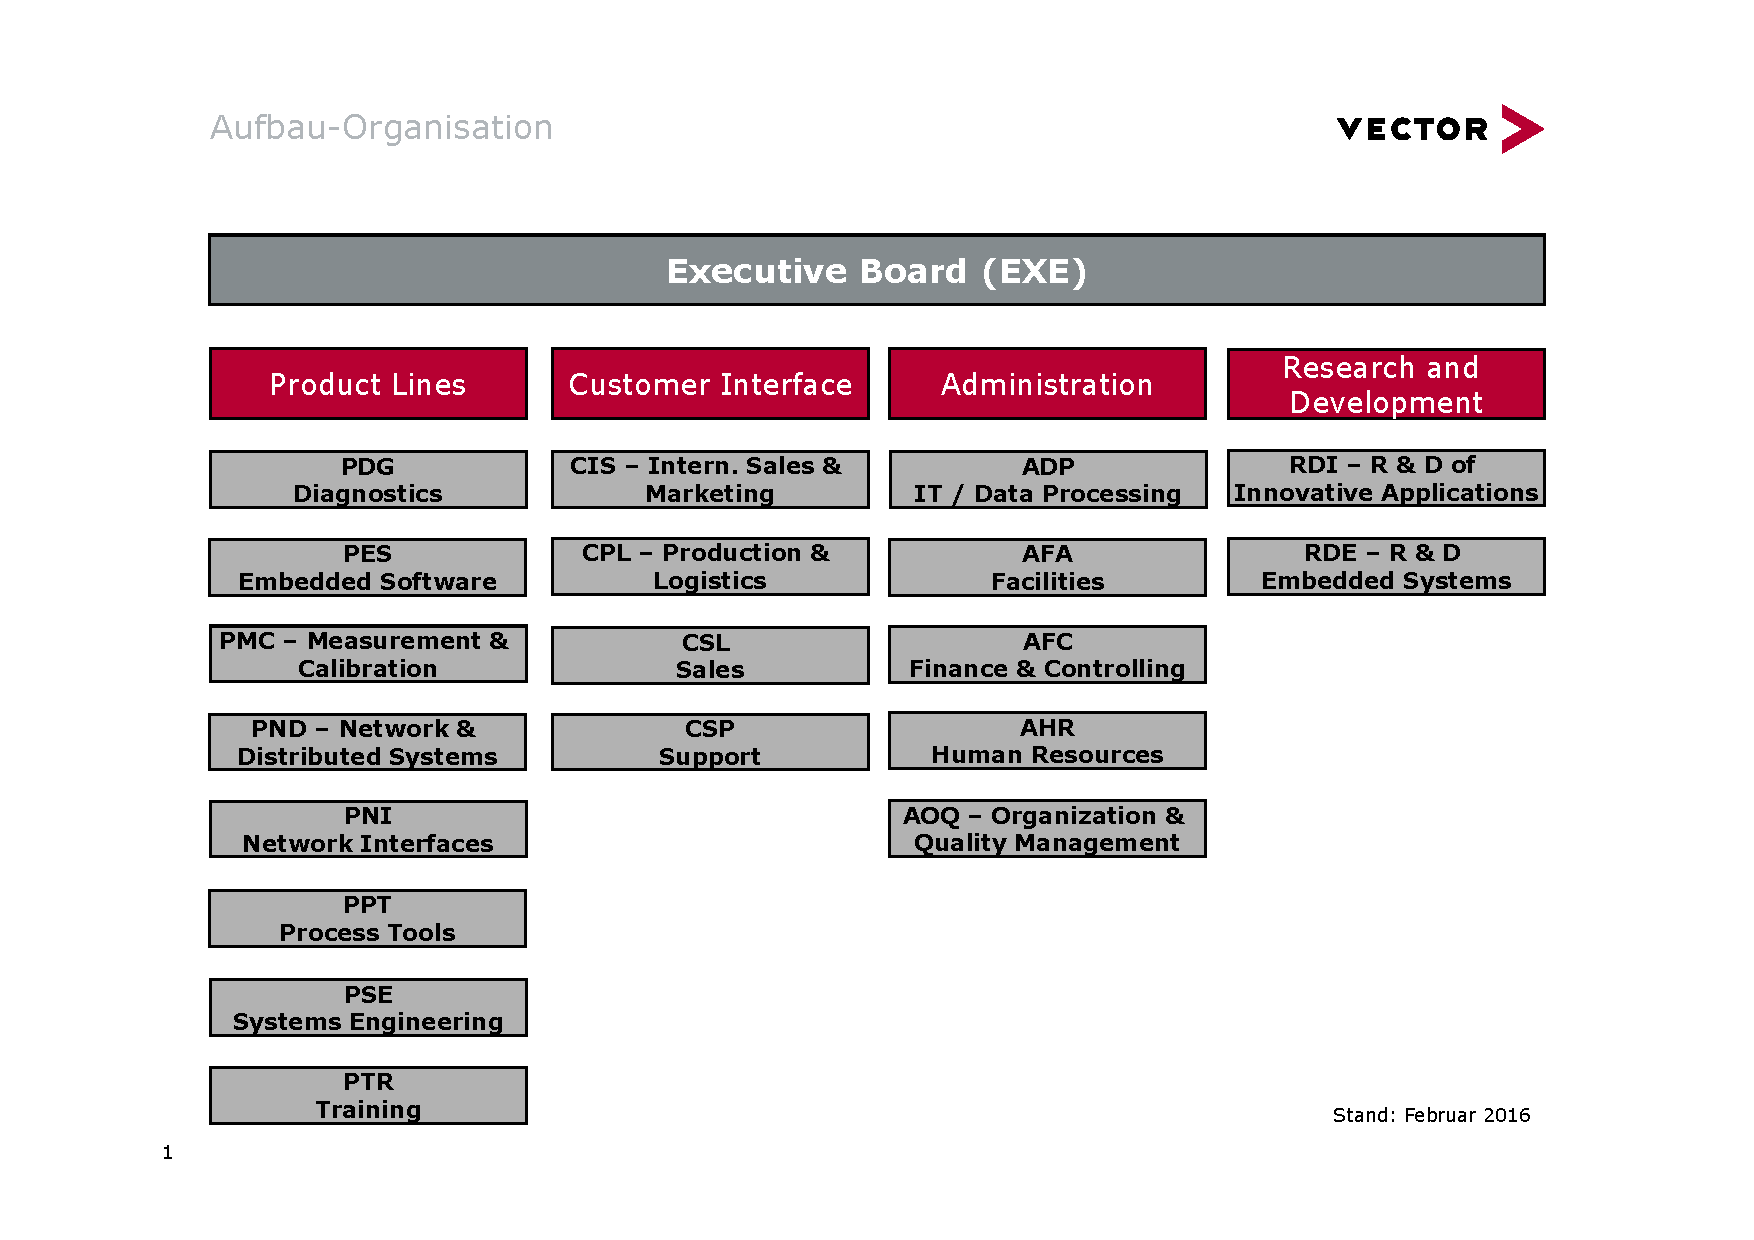
\includegraphics[scale=0.5]{./Bilder/generalstructure_vi.pdf}
\caption{Vectorabteilungen1}
\label{fig:Vectorabteilungen1}
\end{figure}
%


\section{Firmenprofil}\label{cha:firmenprofi}
%
Beschreibung, was in Vector gemacht wird.
\chapter{Beschreibung}
%
\section*{Erste Woche}
%
Am ersten Tag meiner T�tigkeit bei Vector bekam ich die Gelegenheit die Firma und ihre unterschiedlichen Abteilungen n�her kennen zu lernen. Es war erforderlich, an einer ausf�hrlichen Pr�sentation �ber die Firma und die unterschiedlichen Abteilungen teilzunehmen. Dabei konnte ich ebenfalls Mitarbeiter kennen lernen, die genauso wie ich, an diesem Tag mit ihrer Arbeitst�tigkeit bei Vector angefangen haben.

Abbildung \ref{fig:Zeichnung1} zeigt die hierarchische Struktur der einzelnen Unternehmensabbteilungen. Ich durfte w�hrend meiner Paktikumszeit in der PES-Abteilung t�tig sein.
%
\begin{figure}[htp]
\centering
%\def\svgwidth{scale=0.4}
%\input{./Bilder/Zeichnung1.pdf_tex}
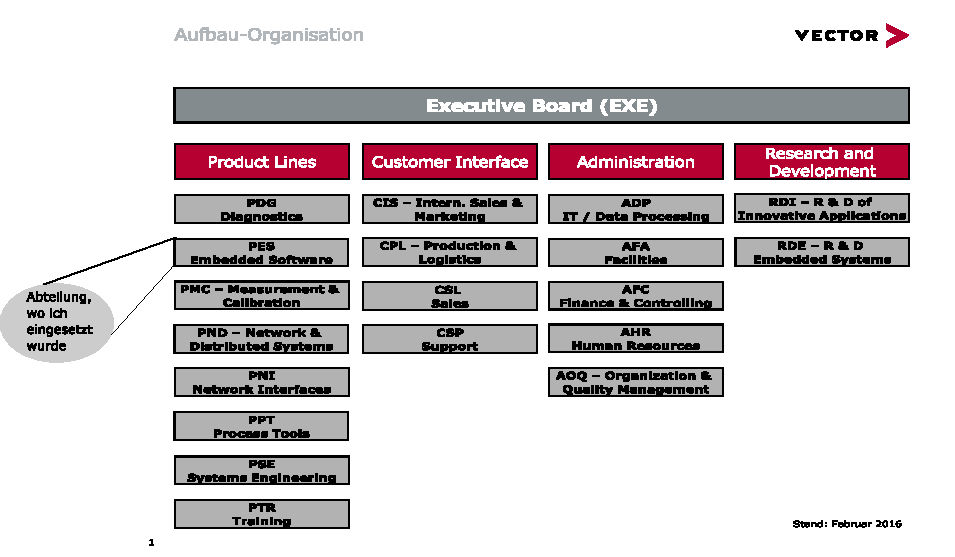
\includegraphics[scale=1]{./Bilder/Zeichnung1.pdf}
\caption{�bersicht der Abteilungen bei der Vector Informatik GmbH}
\label{fig:Zeichnung1}
\end{figure}

W�hrend des Vortrags wurden uns u.a. zahlreiche Einblicke in Themen wie vorhandene Software-Packete, Software-Sicherheit und den richtigen Umgang mit den von Vector zur Verf�gung gestellten Programmen gegeben. 

Mein interner Betreuer, Markus Schwarz, stellte mir anschlie�end die PES Abteilung vor und begleitete mich an meinen Arbeitsplatz.

In den folgenden Tagen galt meine Arbeit der Einarbeitung und Verwendung mancher Software Tools, die von jedem Vector-Mitarbeiter zu verwenden sind. Unter anderem wird dabei eine eigene Umgebung verwendet, um die Arbeitsstunden zu dokumentieren. 

In Abbildung \ref{fig:Tortoisegit} wird ein Ausschnitt von TortoiseSVN-Versionskontroll-Software, die die Vector-Mitarbeiter verwenden, um bei jedem Software-Projekt eine geeinete Versionsverwaltung zu gew�hrleisten. An einer entsprechenden Schulung durfte ich w�hrend der ersten Woche ebenfalls teilnehmen.
%
\begin{figure}[htp]
\centering
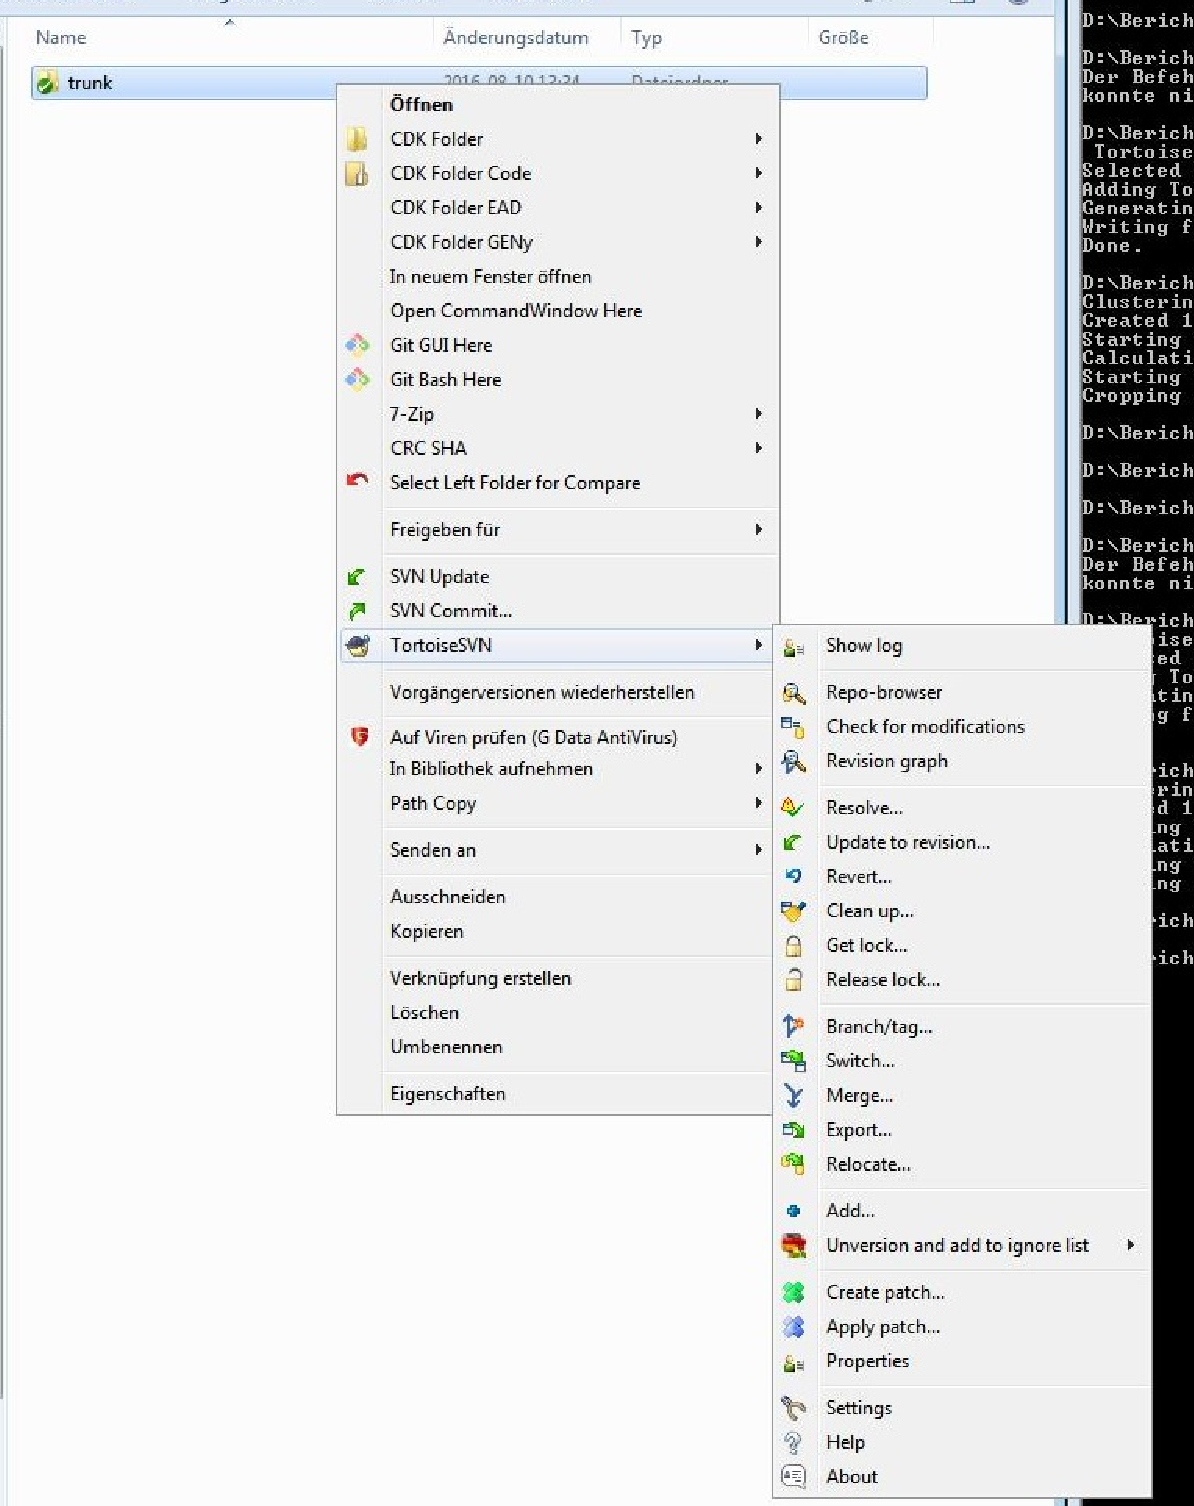
\includegraphics[scale=0.6]{./Bilder/TortoiseSVN.pdf}
\caption{TortoiseSVN wird in Vector zur Versionsverwaltung eingesetzt. Entsprechende Schulungen werden ebenfalls angeboten}
\label{fig:Tortoisegit}
\end{figure}
%
\section{Erste Aufgabenstellung}
%
Innerhalb der ersten Woche wurde mir die 1. Aufgabe meiner Arbeitst�tigkeit bei Vector vorgestellt. Dabei handelt es sich um den MISRA-C-Programmierstandard, �ber den ich mich ausf�hrlich informieren musste. Deshalb wird im Folgenden eine Einleitung in das Thema gegeben.
%Eine genaue Rechnerche �ber die oben erw�hnten Standards war notwendig, um nicht nur einen Einblick in das Thema zu gewinnen sondern auch die technischen Zusammenh�nge zu verstehen. Deswegen wird im folgenden eine kurze Zusammenfassung �ber Themen gegeben, die bei der Einf�hrung des MISRA-Standards eine wichtige Rolle gespielt haben.
%
\paragraph*{\uppercase{MISRA-C-Standard und Gr�nde f�r seine Einf�hrung}}\label{MISRAC}
%
Die Programmiersprache C wurde im Jahr 1972 von Dennis Ritchie und Brian W. Kernighan entwickelt~\cite{CLang}. 

Im Bereich eingebetteter Systeme bietet C den Programmierern vor allem viele M�glichkeiten direkt auf die Speicherbereiche der Hardware zuzugreifen. Dadurch entsteht u.a. die Gefahr, bewusst oder unbewusst viele systemeingene Speicheradressen zu manipulieren und zu einem ungew�nschten Systemverhalten zu f�hren. Weitere kritische Aspekte von C als Programmiersprache k�nnen in~\cite{MasterThMISRA} nachgelesen werden.

Der sogenannte MISRA-C-Standard hilft beispielsweise dabei, den bekannten Nachteilen der Programmiersprache entgegenzuwirken.

MISRA-C hat seinen Ursprung in der Automobilindustrie und wurde durch die britische \glqq The Motor Industry Sofrware Reliability Association\grqq\ eingef�hrt. Die erste Version wurde in 1998 mit dem Ziel ver�ffentlich, eine positive Auswirkung auf die Verwendung eingebetteter Software innerhalb der britischen Automobilindustrie zu haben. Seitdem ist der MISRA-Standard nicht nur im Automobilsektor eingesetzt und bekannt, sondern auch in Bereichen wie Raumfahrtindustrie oder Medizintechnik~\cite{MISRA2004}.

Eine Vielzahl an Regeln sind dabei ver�ffentlicht worden, um robusteren und zuverl�ssigeren Embedded C-Code zu produzieren. Au�erdem wird damit erreicht, dass die erstellten Software-Produkte wiederverwendbar und portabler sind. 

Der zahlreiche Einsatz �ber die Jahre der MISRA-C-2004-Version hat vielf�ltige Erg�nzungen und Verbesserungen als Folge gehabt. Die Regeln sind jetzt bei MISRA-C-2012 so definiert und beschrieben, dass beispielsweise die Begr�ndungen f�r ihre Nutzung umfangreicher wurden~\cite{MISRA2012}. 
%
\paragraph*{\uppercase{MISRA-C-Standard in der Vector Informatik GmbH}}\label{MISRAC}
%
Zur Verifikation der MISRA-C-Kodierungsregeln wird, wie in Abbildung \ref{fig:MISRA} zu sehen, zus�tzlich von Vector ein Dokument verwendet (Gemeinsames Subset der MISRA-C-Guidelines), in dem der HIS-Arbeitskreis-Softwaretest im Jahr 2006 f�r die MISRA-Guidelines Version 2004 eine gemeinsame Untermenge der anwendbaren Regeln festgelegt hat~\cite{HIS_Standard}. Die in diesem Dokument erw�hnten Vorschriften bez�glich der MISRA-Regeln m�ssen bei der Herstellung und Lieferung eingebetteter Software eingehalten werden.
 
Um dies zu gew�hrleitsten, richtet sich Vector bei der Erstellung eingebetteter Software nach einer festgelegten Anleitung zum korrekten Programmierstil und vorgegebenen Code-Template-Files, bei denen die oben genannten Anforderungen erf�llt sind. Da diese Templates erweitert werden, ist eine �berpr�fung der MISRA-Kodierungsregeln trotzdem durchzuf�hren. In einer sogenannte Compliance-Matrix wird festgelegt, auf welcher Art und Weise die einzelnen, relevanten MISRA-Regeln gepr�ft werden sollten. Hierbei kommen verschiedene statische Analysetools oder die jeweiligen Compiler in Frage. Ist die Einhaltung einer einzelnen Regel nicht komplett durch ein solches Tool automatisiert �berpr�fbar, dann ist man auf eine manuelle �berpr�fung angewiesen~\cite{MISRA2012}.

Vector richtet sich momentan bei der Erstellung eingebetteter Software noch nicht nach der aktuellen MISRA-C-2012-Version~\cite{MISRACodeMetric}. 

Der Hauptgrund liegt darin, dass bei diesem neuen Standard viele �nderungen bei der Definition, Struktur und Aufbau der Regeln aufgetreten sind. Das bedeutet, dass sich ein Umstieg von der letzten MISRA-C-2004-Version auf die aktuelle Version nicht durchf�hren l�sst, ohne davor einen entsprechenden Aufwand zu investieren.
%
\begin{figure}[!htp]
\centering
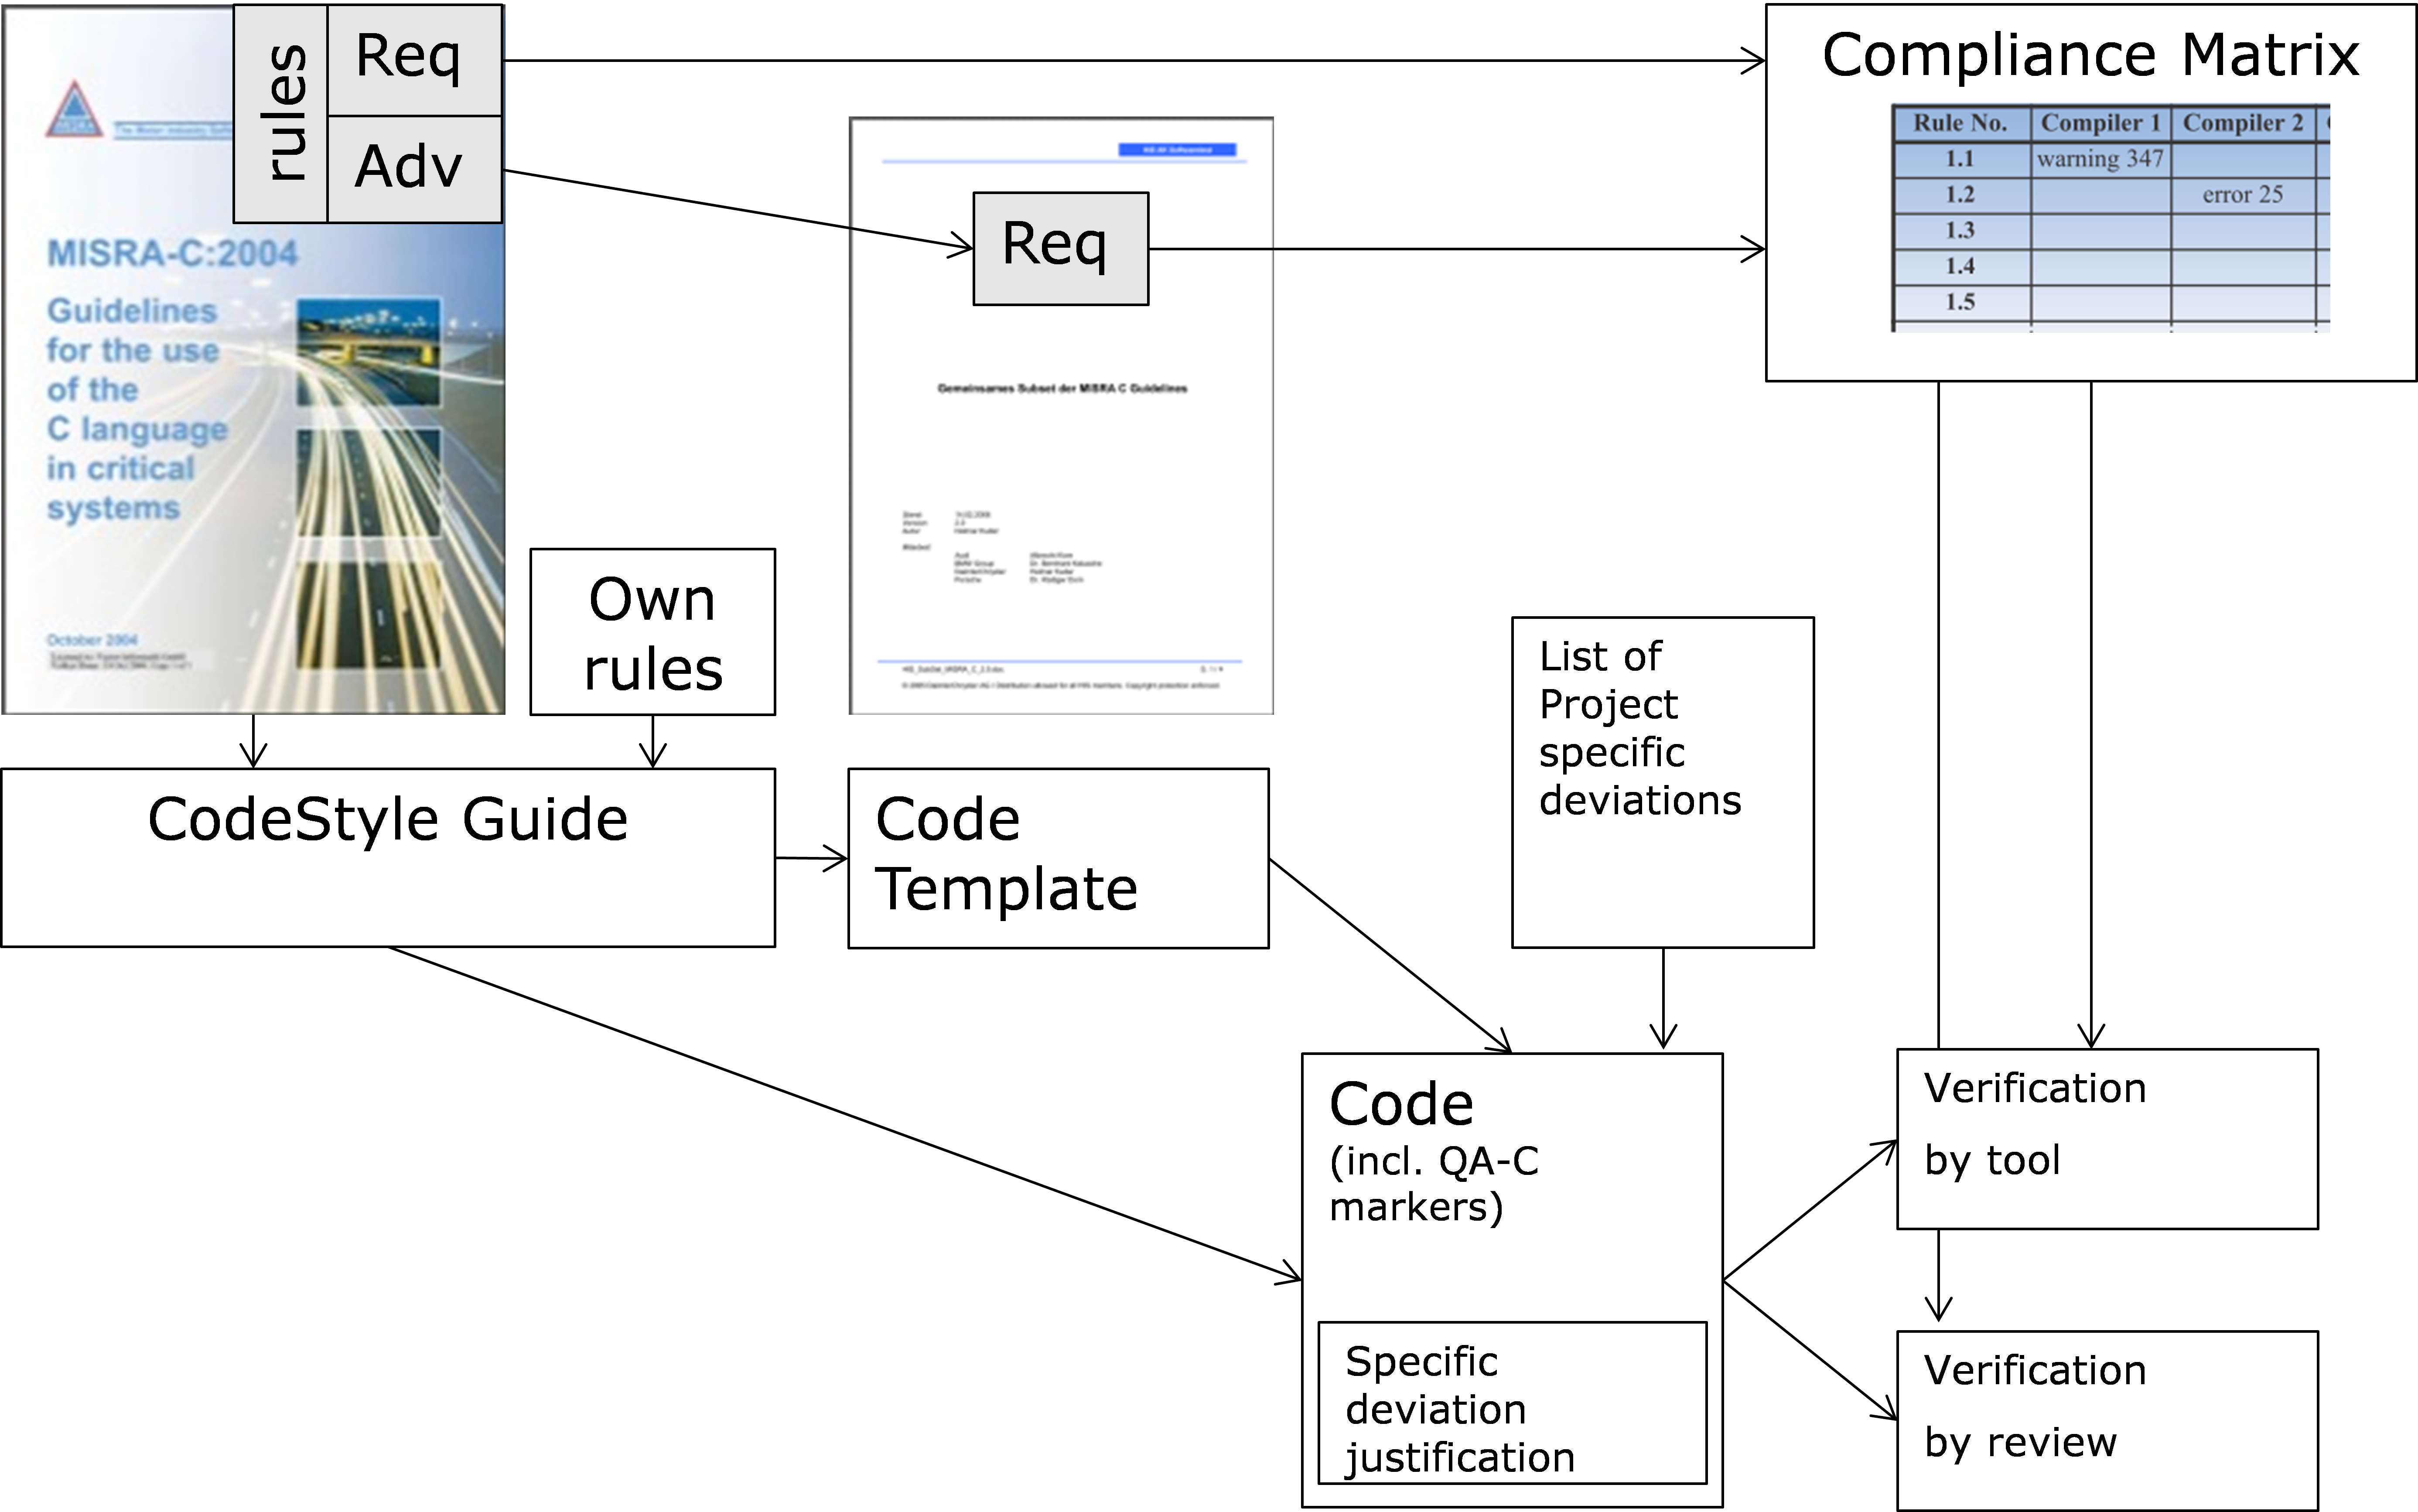
\includegraphics[scale=0.1]{./Bilder/MISRAoverall.png}
\caption{Struktur der bei Vector durchgef�hrten statischen Codeanalysen. Entnommen aus~\cite{MISRACodeMetric}.}
\label{fig:MISRA}
\end{figure}
%

Die OEMs fragen seit der Einf�hrung von MISRA-C-2012 nach, dass die in ihren Produkten eingesetzten Embedded-Software mit dieser Version des Standards konform geht.
Vector und somit die Abteilung PES sind aus den genannten Gr�nden darauf angewiesen, in naher Zukunft einen Umstieg in die neue Version zu erm�glichen. 
%
\begin{Aufgabenstellung}
besteht darin, sich erstens mit den Konzepten des MISRA-C Kodierungsstandards vertraut zu machen. Anschlie�end sollten m�gliche R�ckschl�sse gezogen werden, wie umfangreich ein Umstieg von dem aktuell in der Firma gepr�ften Kodierungsstandard MISRA-C-2004 in den neuen Standard MISRA-C-2012 ist.
\end{Aufgabenstellung}
%
Eine detaillierte Analyse vor allem �ber die Kompatibilit�t zwischen den beiden Versionen (2004 und 2012) wird innerhalb der kommenden Wochen durchgef�hrt. Die Ergebnisse dieser ersten Vorarbeiten k�nnen als Grundlage weiterer Untersuchungen dienen.
%
\clearpage
\section*{Zweite Woche}
%
\section{Durchf�hrung der ersten Aufgabenstellung}
%
Eine genaue Rechnerche �ber die oben erw�hnten Standards war notwendig, um nicht nur einen Einblick in das Thema zu gewinnen sondern auch die technischen Zusammenh�nge zu verstehen.
%
\paragraph*{\uppercase{MISRA-C-2012}}
%
Im Gegensatz zu den ersten MISRA-Versionen fordert MISRA C:2012, dass programmiertes C Code mit dem Standard \textsc{C99} \footnote{ISO Standard for the C language ISO/IEC 9899:1999~\cite{MISRA2012}} konform geht. Au�erdem sind einige neue Regeln hinzugekommen, die sich haupts�chlich auf \textsc{C99} beziehen, einige wenige wurden umformuliert oder sogar entfernt~\cite{WarMISRAC}.

Bei den ersten MISRA-Versionen sind die Regeln in zwei Kategorien eingeteilt: 
notwendige (required) und empfohlene (advisory) Regel. Die ersten sind erforderliche Anforderungen an dem Programmierer. Die empfohlenen Regeln k�nnen eingehalten werden, dies ist aber nicht unbedingt notwendig.

Die einzelnen Regeln bestehen jetzt bei MISRA-C-2012 aus mehreren Teilen:

\begin{itemize}
\item Erweiterte Erl�uterungen (Amplification): \\
Eine umfangreichere Beschreibeung der betrachteten Richtlinie.
\item Begr�ndung (Rationale): \\
Erl�uterung, warum die Regel ben�tigt wird.
\item Ausnahmen (Exceptions): \\
Beschreibung der F�lle, bei denen die betrachtete Regel nicht gilt.
\item Beispiele (Examples): \\
Beispiele, wie man die Regel anwenden kann.
\end{itemize}

\textsc{MISRA-C-2012} hat somit eine zus�tzliche Kategorie eingef�hrt, n�mlich die zwingend erforderliche Regel (mandatory). Unter keinen Umst�nden d�rfen solche Regel verletzt werden.

Dem Begriff der Durchsetzbarkeit einer Regel wurde besondendere Aufmerksamkeit geschenkt. Die Durchsetzbarkeit besagt, wie gut sich eine Regel mithilfe einer statischen Analyse pr�fen l�sst. Letzteres ist von hoher Bedeutung, denn die automatische Pr�fung von Regeln spart viel Zeit, wirkt sofort, ist zuverl�ssig, wiederholbar und konsistent~\cite{WarMISRAC}. Au�erdem ist die Durchsetzbarkeit ein Ma� daf�r, wie abh�ngig ein bestimmmtes Entwicklungsprozess von der manuellen Codeanalyse ist.

Die Ma�nahmen, die diesbez�glich bei der neuen MISRA-Version getroffen wurden, sind im Folgenden erl�utert\footnote{Siehe dazu~\cite{MISRA2012}, Unterkapitel 6.6}:

\begin{itemize}
\item Es besteht nun ein Unterschied zwischen Regeln und Anordnungen (Directives). Regeln lassen sich direkt durch eine Analyse des Quellcodes durchsetzen. Anordnungen sind im Gegensatz dazu nicht pr�zise definiert, so dass ihre Einhaltung  eine genauere Untersuchung u.a. der Funktionsanforderungen ben�tigt.
\item Eine Regel kann innerhalb einer \textit{einzelnen �bersetzungseinheit} (Single Translation Unit) oder eines \textit{Systems} (System) analysiert werden. Diese beiden Begriffe geben den n�tigen Aufwand einer Analyse wieder, um eine Regel zu �berpr�fen.
\end{itemize}

Abbildung \ref{fig:MISRA2004} gibt die wichtigsten Eigenschaften und Unterschiede zwischen den relevanten MISRA-Versionen wieder.
%
\begin{figure}[!htp]
\centering
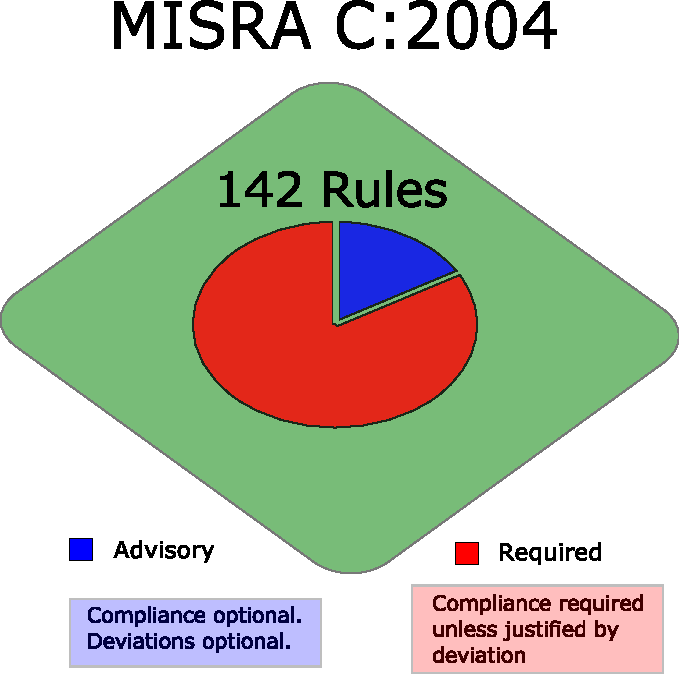
\includegraphics[scale=0.7]{./Bilder/MISRA2004.pdf}
\caption{Vergleich zwischen den aktuellen MISRA-C-Versionen. In Anlehnung an~\cite{WarMISRAC}}
\label{fig:MISRA2004}
\end{figure}
%
\clearpage
\section*{Dritte Woche}\label{sec:DritteWoche}
%

%
Um den Nachweis liefern zu k�nnen, wie konform ein spezifisches Software-Projekt mit dem gesamten MISRA-C-Regelwerk geht, wird in der Regel ein ausgew�hltes statisches Analysewerkzeug eingesetzt. 
%
\paragraph*{Verwendetes statisches Analysewerkzeug QA-C}\label{QAC7Einf}
%
Bei Vector wird zurzeit das Programm QA-C der Firma QA-Systems verwendet, um die statischen Code-Analysen bei ihren Software-Produkten durchzuf�hren~\cite{MISRACodeMetric}. Das genannte Tool ist eine kommerzielle Software zur automatisierten �berpr�fung eines fetgelegten und firmenspezifischen Programmierstandards~\cite{QAC_Iseite}.

QA-C bietet die M�glichkeit eine statische Code-Analyse in 3 Phasen durchzuf�hren. In der 1. Phase der Analyse wird der Quellcode auf Konformit�t mit definierten Standards wie beispielsweise \textsc{C99} untersucht. Die drauf folgende Analyse (secondary analysis) ist ein optionale Erweiterung, bei der sich in der Regel industrie-, firmeneigene oder standardspezifische Tests durchf�hren lassen (MISRA-C-2004 bzw. MISRA-C-2012). In der dritten Phase wird die so genannte cross-module-Analyse durchgef�hrt, welche die aus dem Source Code extrahierten \textit{translation units} untersucht. F�r eine genaue Beschreibung der QA-C-Funktionali�ten sei auf~\cite{QAC70WinUserGuide} verwiesen. 

Abbildung \ref{fig:QACfunc} zeigt einen �berblick �ber die funktionalen Beziehungen der Analyse-Software und die unterschiedlichen Ergebnisse einer beliebigen Beispielanwendung.

%
\begin{figure}[!htp]
\centering
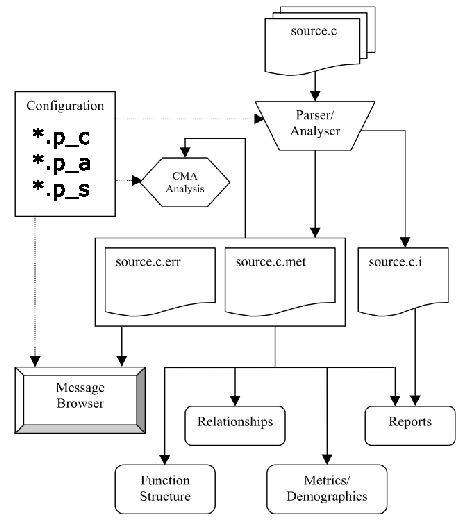
\includegraphics[scale=1.2]{./Bilder/QAC_functions.pdf}
\caption{Funktionale Beziehungen bei der Verwendung vom QA-C-Analysetool. In Anlehnung an~\cite{QAC70WinUserGuide}.}
\label{fig:QACfunc}
\end{figure}
%

Dabei kann man erkennen, dass beim Teil \textit{Configuration} bestimmte Files notwendig sind, damit ein QA-C-Projekt initialisiert und �berhaupt die Analyse stattfinden kann. Diese Einstellungsdateien werden als \textit{personalities} bezeichnet und im Folgenden n�her beschrieben: 

\begin{itemize}
\item Compiler Personality ($*.p\_c$): \\
definiert die Einstellungen f�r den verwendeten Compiler. 
\item Analysis Personality ($*.p\_a$): \\
definiert die Analyse-Einstellungen, die projektabh�ngig sind wie die Include-Pfade der zu analysierenden Files.  
\item Message Personality ($*.p\_s$): \\
Einstellungen bez�glich der f�r die Untersuchung relevanten QA-C-Nachrichten.
\end{itemize}

Die Struktur bzw. der Aufbau der obigen Dateien wird vom Hersteller (QA-Systems) vorgegeben. Man ist deswegen zur korrekten Anwendung auf die Dokumentation der Software angewiesen. 

Ich durfte eigenst�ndig eine statische Analyse einer einzelnen BSW-Komponente (Single Component) mit der betrachteten QA-C-Software durchf�hren und dabei die oben eingef�hrten Einstellungsdateien verwenden bzw. eingeben. Die Analyse erfolgte mithilfe der Version QA-C 7.0, f�r die die Abteilung �ber Lizenzen verf�gt. Die Analysen, die mit QA-C durchgef�hrt werden k�nnen, beschr�nken sich nicht auf Kodierungsregeln wie beispielsweise die MISRA-C-Regeln. Dabei lassen sich auch funktionale und technische Fehler, potentielle Bugs sowie auch qualitative Schwachstellen im Code~\cite{QAC70WinUserGuide} erkennen. 

Die entsprechenden Ergebnisse dieser einf�hrenden Analyse sind in \figref{fig:QAC7Single1} bzw. \figref{fig:QAC7Single} dargestellt. Wenn gem�� der vorgenommenen Einstellungen keine Findings auftreten, gehen die analysierten Files mit den vorgegebenen Kodierungsstandards komform.
%
\begin{figure}[!htp]
\centering
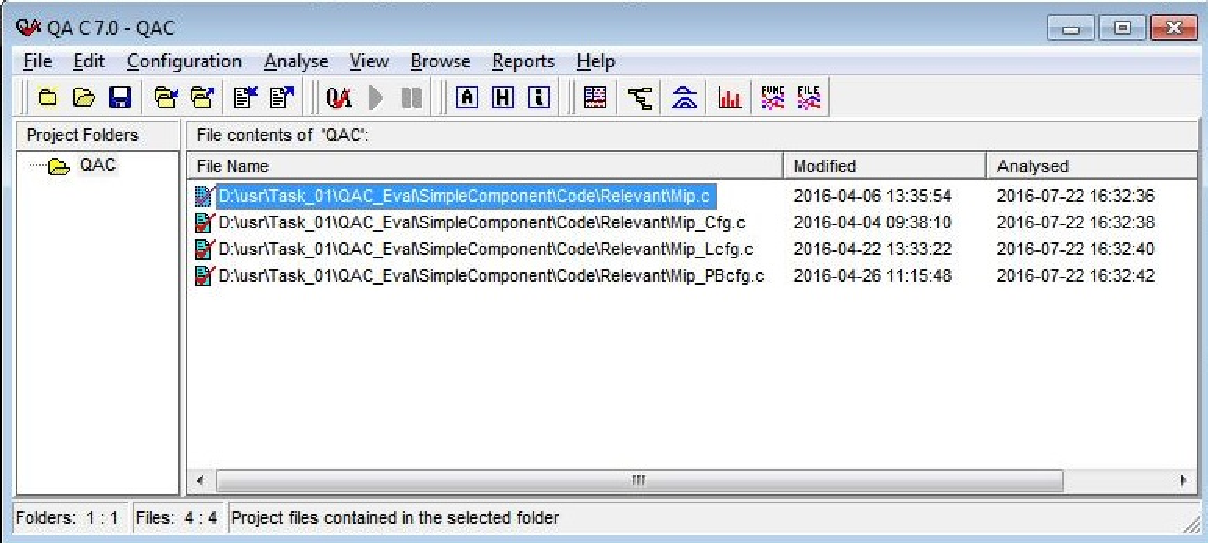
\includegraphics[scale=0.7]{./Bilder/QAC7Single1.pdf}
\caption{Analyse einer ersten BSW-Komponente mit QA-C7.}
\label{fig:QAC7Single1}
\end{figure}
%
\begin{figure}[!htp]
\centering
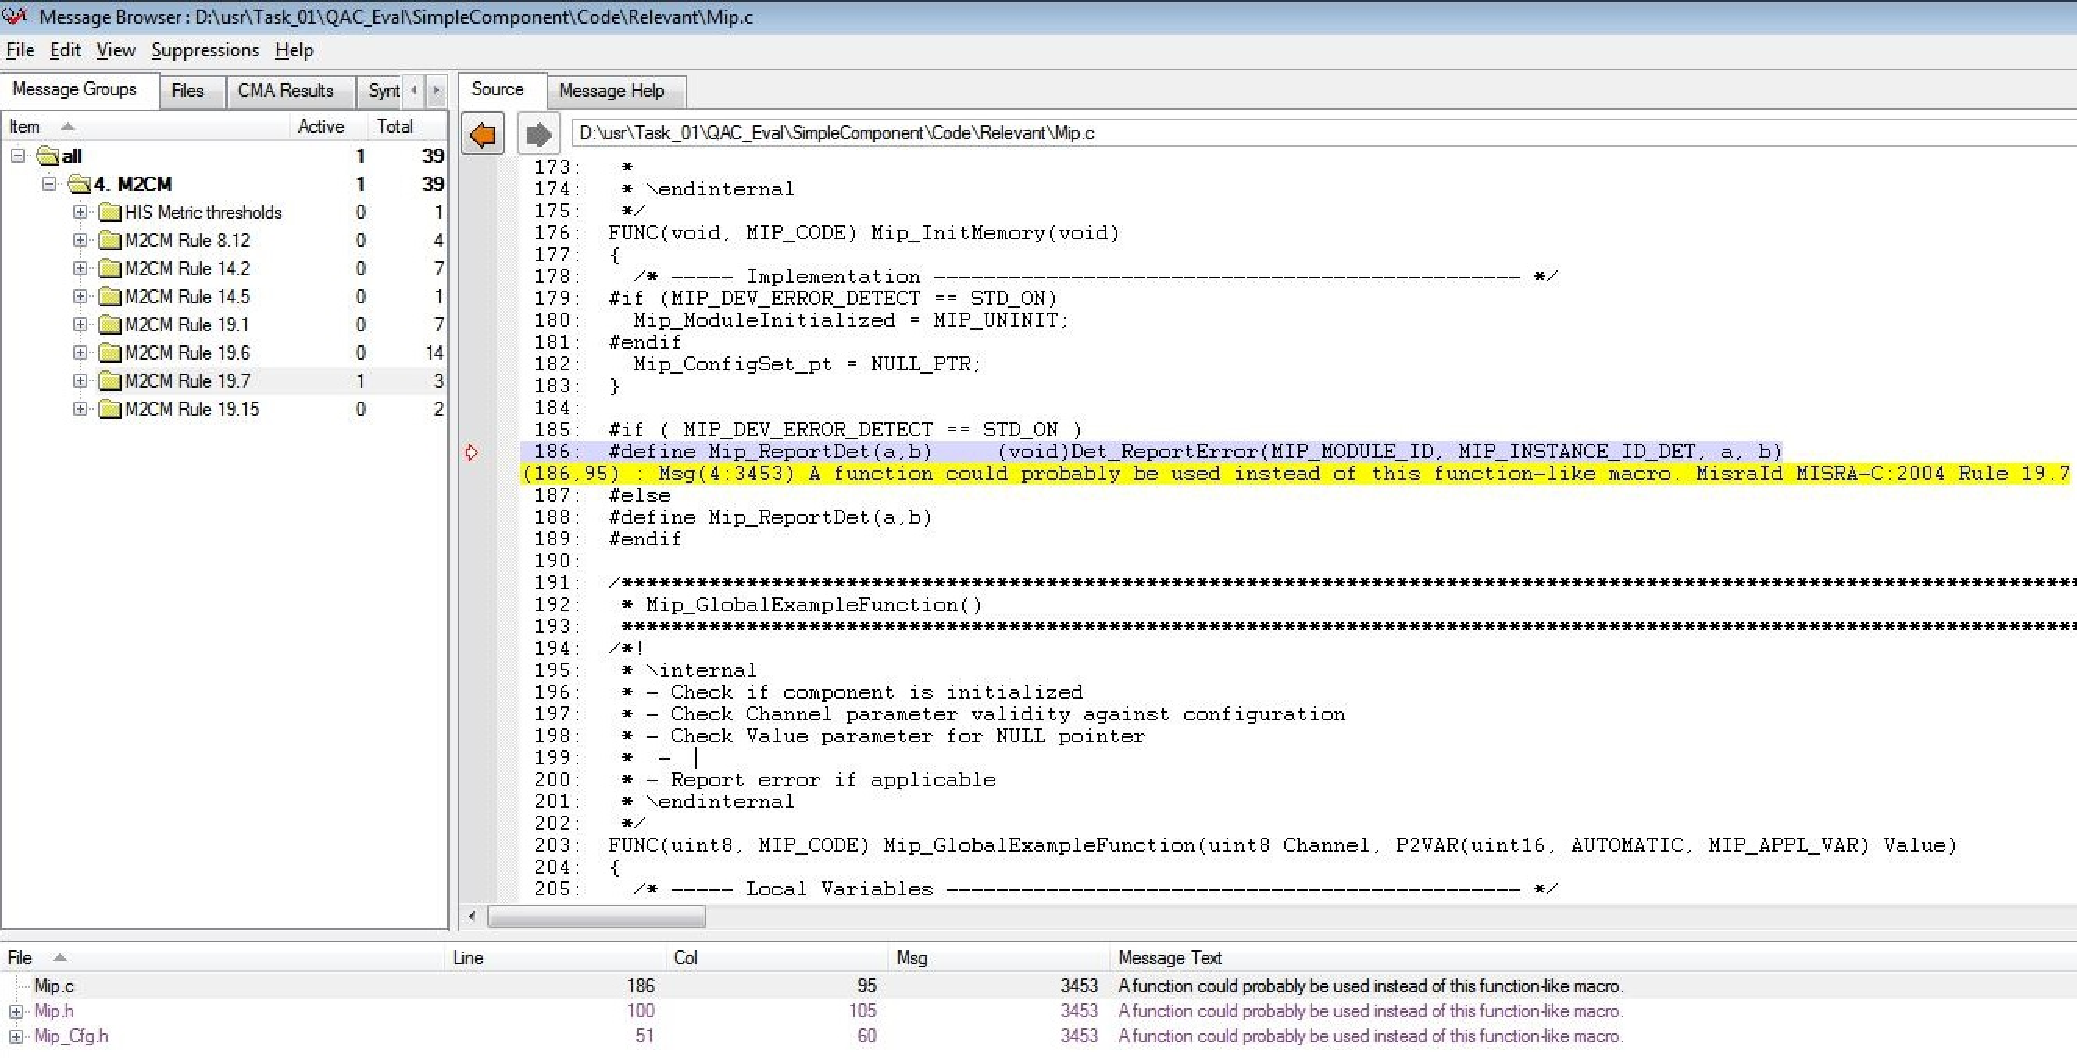
\includegraphics[scale=0.45]{./Bilder/QAC7Single.pdf}
\caption{Ergebnisse der Analyse vom betrachteten Source Code.}
\label{fig:QAC7Single}
\end{figure}
%
\clearpage
Um die Analyse des Projekts zu starten, wurden die folgenden Listings erstellt: 
%
\begin{lstlisting}[basicstyle=\ttfamily\scriptsize, caption = {Compiler personality file QA-C.p\_c}, label={lst:QAC_p_c}]
-i "C:\Program Files (x86)\Microsoft Visual Studio 10.0\VC\Include" 
-i "C:\Program Files (x86)\Microsoft SDKs\Windows\v7.0A\Include" 
-q "C:\Program Files (x86)\Microsoft Visual Studio 10.0\VC\Include" 
-q "C:\Program Files (x86)\Microsoft SDKs\Windows\v7.0A\Include" 
-it "ptrdiff_t=int"
-it "wchar_t=unsigned short"
-d "__alignof(type)=1"
-d "__based(type)="
-d "__cdecl="
-d "__COUNTER__=1"
-d "__declspec(arg)="
-d "__declspec=_ignore_paren"
-d "__event="
-d "__far="
-d "__fastcall="
-d "__forceinline=inline"
-d "__FUNCDNAME__=__FUNCTION__"
-d "__FUNCSIG__=__FUNCTION__"
...
\end{lstlisting}

\begin{lstlisting}[basicstyle=\ttfamily\scriptsize, caption = {Analysis personality file QA-C.p\_s}, label={lst:QAC_p_s}]
-rem "ShellExe=C:\Program Files (x86)\PRQA\QAC-7.0\m2cm\bin\qacsa_m2cm.exe"
-rem "EnablePostAnalysis=1"
-rem "ShellParams=%Q %F -forget cmaf"
-up "d:\uti\CDK\Tools\QAC\m2cm\messages\" 
-usr .m2cm
-l+
-format "%?u==0%(%q%:%?F%(%F%)%)(%l,%c) : %?u==0%(%?h%(Err%:Msg%)%:-->%)(%g:%N) %R(%u,  )%t MisraId %v"
-max 0
-m+
-st+
-hdr-
-summary-
-references+
-onelineonly-  
-hiddenwarnings-

-o 9
-o 40
-o 41
-o 42
-o 97
-o 159
...
\end{lstlisting}

\begin{lstlisting}[basicstyle=\ttfamily\scriptsize, caption = {Message personality file QA-C.p\_a}, label={lst:QAC_p_a}]
-il 0
-i "D:\usr\Task_01\QAC_Eval\SimpleComponent\Code\Relevant"                    
-i "D:\usr\Task_01\QAC_Eval\SimpleComponent\Code\Includes"                    
-q "D:\usr\Task_01\QAC_Eval\SimpleComponent\Code\Includes"         
-d "__MSVC_RUNTIME_CHECKS"
-d "_CHAR_UNSIGNED"
-d "_CONSOLE"
-d "_CPPRTTI"
-d "_DEBUG"
-d "_DLL"
-d "_MT"
-d "_UNICODE"
-d "CDK_CHECK_MISRA"
-d "UNICODE"
-d "VECTOR_DEBUG"
-sty exdented
-tab 2
-en ASC
-maxerr 0
...
\end{lstlisting}

Mithilfe dieser Dateien fiel es mir einfacher zu verstehen, wie die genannten Einstellungen �ber die \textit{personality files} durchzuf�hren sind. In \lstref{lst:QAC_p_c} l�sst sich beispielweise erkennen, wie bei den QA-C-Compiler-Optionen �ber den Platzhalter $-i$ die Suchpfade f�r den beim analysierten Projekt verwendeten Compiler vorgegeben werden. Analog lassen sich projektabh�ngige Include-Pfade am Anfang der \textit{personality file} QA-C.p\_a (siehe \lstref{lst:QAC_p_a}) angeben.

Im Gegensatz zur QA-C vorgestellten Version 7.0 werden von der 9.0 Version beide relevanten Versionen des MISRA-Standards (2004 und 2012) unterst�tzt. Eine genaue Beschreibung dazu wird im folgenden Kapitel gegeben.
%
\paragraph*{L�sungsansatz zum Vergleich der relevanten MISRA-Versionen}
%
Das Ziel, welches man beim L�sen dieser Aufgabe verfolgt, ist eine Schlussfolgerung daraus zu ziehen, ob ein Umstieg auf den aktuellen MISRA 2012-Standard mit vertretbarem Aufwand m�glich ist. Beim genannten Umstieg geht es vor allem um die Frage, ob die Struktur der Software-Produkte, die bisher bei Vector erstellt wurden, beibehalten werden kann oder diese wegen neu eingef�hrter bzw. ge�nderter MISRA-Regeln anzupassen ist. 

Als Beurteilungskriterium k�nnten die Ergebnisse eines Vergleichs zwischen den betrachteten MISRA C- bzw. QA-C-Versionen dienen. W�rde man dabei feststellen, dass in den neuen Versionen keine gro�en �nderungen in der Definition oder Unterst�tzung der Regeln vorkommen, dann w�re der Umstieg unproblematisch m�glich. Sind im Gegenteil dazu viele MISRA-Regeln bzw. viele der von QA-C gepr�ften Regeln neu hinzugekommen, gel�scht oder umgestrukturiert worden, dann w�rde der dabei entstehende Aufwand ansteigen.

Um eine erste Analyse durchzuf�hren, sollten erstens die Unterschiede der beiden betrachteten MISRA Standards genauer untersucht und gegen�ber gestellt werden. Zweitens  sind die QA-C Versionen 7.0 und (die aktuelle) 9.0 in Bezug auf unterst�tzte Regeln und Toolnutzung miteinander zu vergleichen. Der Zweiter Punkt ist wichtiger im Bezug auf den oben genannten Umstieg zwischen den MISRA-Versionen, wie in den folgenden Kapitel erl�urtert wird.

%Wie schon oben einf�hrend erw�hnt verf�gt die PES-Abteilung �ber eine Lizenz der QA-C 7.0-Version, mit deren Hilfe die Konformit�t von eingebetteter Software mit dem MISRA-C:2004-Standard gepr�ft wird. 
\newpage
%
\section*{Vierte Woche}\label{sec:VierteWoche}
%
Im Gegensatz zu den von QA-C verwendeten Richtlinien zur Pr�fung von MISRA-Regeln braucht man kein direkter Vergleich der MISRA-Versionen durchzuf�hren. Ein entsprechender Ansatz wurde bereits von der britischen \glqq The Motor Industry Sofrware Reliability Association\grqq~ver�ffentlicht~\cite{Addendum1}. Eine Registrierung auf der Internetseite der MISRA-Institution ist erforderlich gewesen, um Zugang zum Dokument zu erlangen.

In \figvref{fig:Addendum1} ist ein kleiner Abschnitt des genannten Dokuments zu sehen, wo die Gegen�berstellungen der beiden betrachteten MISRA-Standards gezeigt sind. 

%
\begin{figure}[!htp]
\centering
\includegraphics[scale=0.45]{./Bilder/Addendum1.pdf}
\caption{Rule mapping MISRA C:2004 $\rightarrow$ MISRA C:2012. In der vorliegenden Abbildung werden die relevanten �nderungen und Zusammenh�nge zwischen den alten und den neuen MISRA-C-Regeln. Entnommen aus ~\cite{Addendum1}.}
\label{fig:Addendum1}
\end{figure}
%
%%
%\begin{figure}[htp]
%\centering
%\includegraphics[scale=0.75]{./Bilder/Addendum2.pdf}
%\caption{Rule mapping MISRA C:2012 $\rightarrow$ MISRA C:2004. Entnommen aus ~\cite{Addendum1}}
%\label{fig:Addendum2}
%\end{figure}
%%
\newpage
In \tabvref{tab:TabMisra1} bzw. \tabvref{tab:TabMisra2} werden die Ergebnisse einer ersten groben Analyse des in Abbildung \ref{fig:Addendum1} gezeigten Dokuments angegeben. Dabei ist zu erkennen, dass sowohl das Mapping \linebreak MISRA-C-2004 $\rightarrow$ MISRA-C-2012 als auch MISRA-C-2012 $\rightarrow$ MISRA-C-2004 wichtige Hinweise auf Ver�nderungen der Regeln liefern k�nnen. Die Bewertungskriterien sind so gew�hlt, dass diese eine gemeinsame Eigenschaft der neuen bzw. alten Regeln wiederspiegeln. 
%
\begin{longtable}{|l|l|}
\hline
\textbf{Eigenschaft der Regel} & \textbf{Anzahl an betroffenen Regeln} \\
\endhead
\hline
Gel�scht & 9 \\
\hline
<group prefix>-Nummer gleich geblieben & 38\\
\hline
<group prefix>-Nummer ge�ndert & 95\\
\hline
Regel wurde in einzelnen Regeln unterteilt & 15 \\
\hline
Regel wurde in Anordnung (directive) &\\umgewandelt & 19 \\
\hline
\caption{Relevante Zusammenh�nge aus Rule-Mapping MISRA-C-2004 $\rightarrow$ MISRA-C-2012.}
\label{tab:TabMisra1}
\end{longtable}
%
\begin{longtable}{|l|l|}
\hline
\textbf{Eigenschaft der Regel} & \textbf{Anzahl an betroffenen Regeln} \\
\endhead
\hline
neu eingef�hrt & 37\\
\hline
Regel fasst mehrere alte Regeln zusammen & 19 \\
\hline
\caption{Relevante Zusammenh�nge aus Rule mapping MISRA-C-2012 $\rightarrow$ MISRA-C-2004. Das Ziel der erstellten Tabellen ist, wichtige Eingenschaften bei den durchgef�hrten �nderungen zwischen den betrachteten MIRSA-C-Versionen zu erkennen. Diese beiden Analysen wurde h�ndisch durchgef�hrt.}
\label{tab:TabMisra2}
\end{longtable}
%

Eine weitere Untersuchung �ber die Unterschiede zwischen den MISRA-Versionen war mithilfe des genannten Addendum-Dokuments nicht notwendig. 

Vielmehr sollte man sich auf die im Laufe der Zeit durchgef�hrten �nderungen zwischen QA-C-Versionen konzentrieren, da �ber dieses Tool die MISRA-C-Regeln bei den Projekten in Vector gepr�ft werden. 

Ziel ist es somit, einen Weg zu finden, um bestimmte Muster festzulegen, die die relevanten �nderungen zwischen den Versionen 7.0 bis 9.0 m�glichst gut wiedergeben.

Werden viele �nderungen bei der Toolnutzung und der in QA-C unterst�tzten MISRA-Pr�fung festgestellt, dann kann sich der gew�nschte automatisierte Umstieg als umst�ndlich erweisen.

Bei der Analyse werden 6 relevante \textit{release notes} ausgew�hlt und einer ausf�hrlichen Analyse unterzogen. Diese Dokumente beschreiben sehr gut den erw�hnten �nderungsverlauf.

Die in \figvref{fig:QAC7_9Zusam} gezeigte Excel-Tabelle zeigt das Ergebnis der durchgef�hrten Untersuchung.
%
\begin{landscape}
\begin{figure}[!htp]
\centering
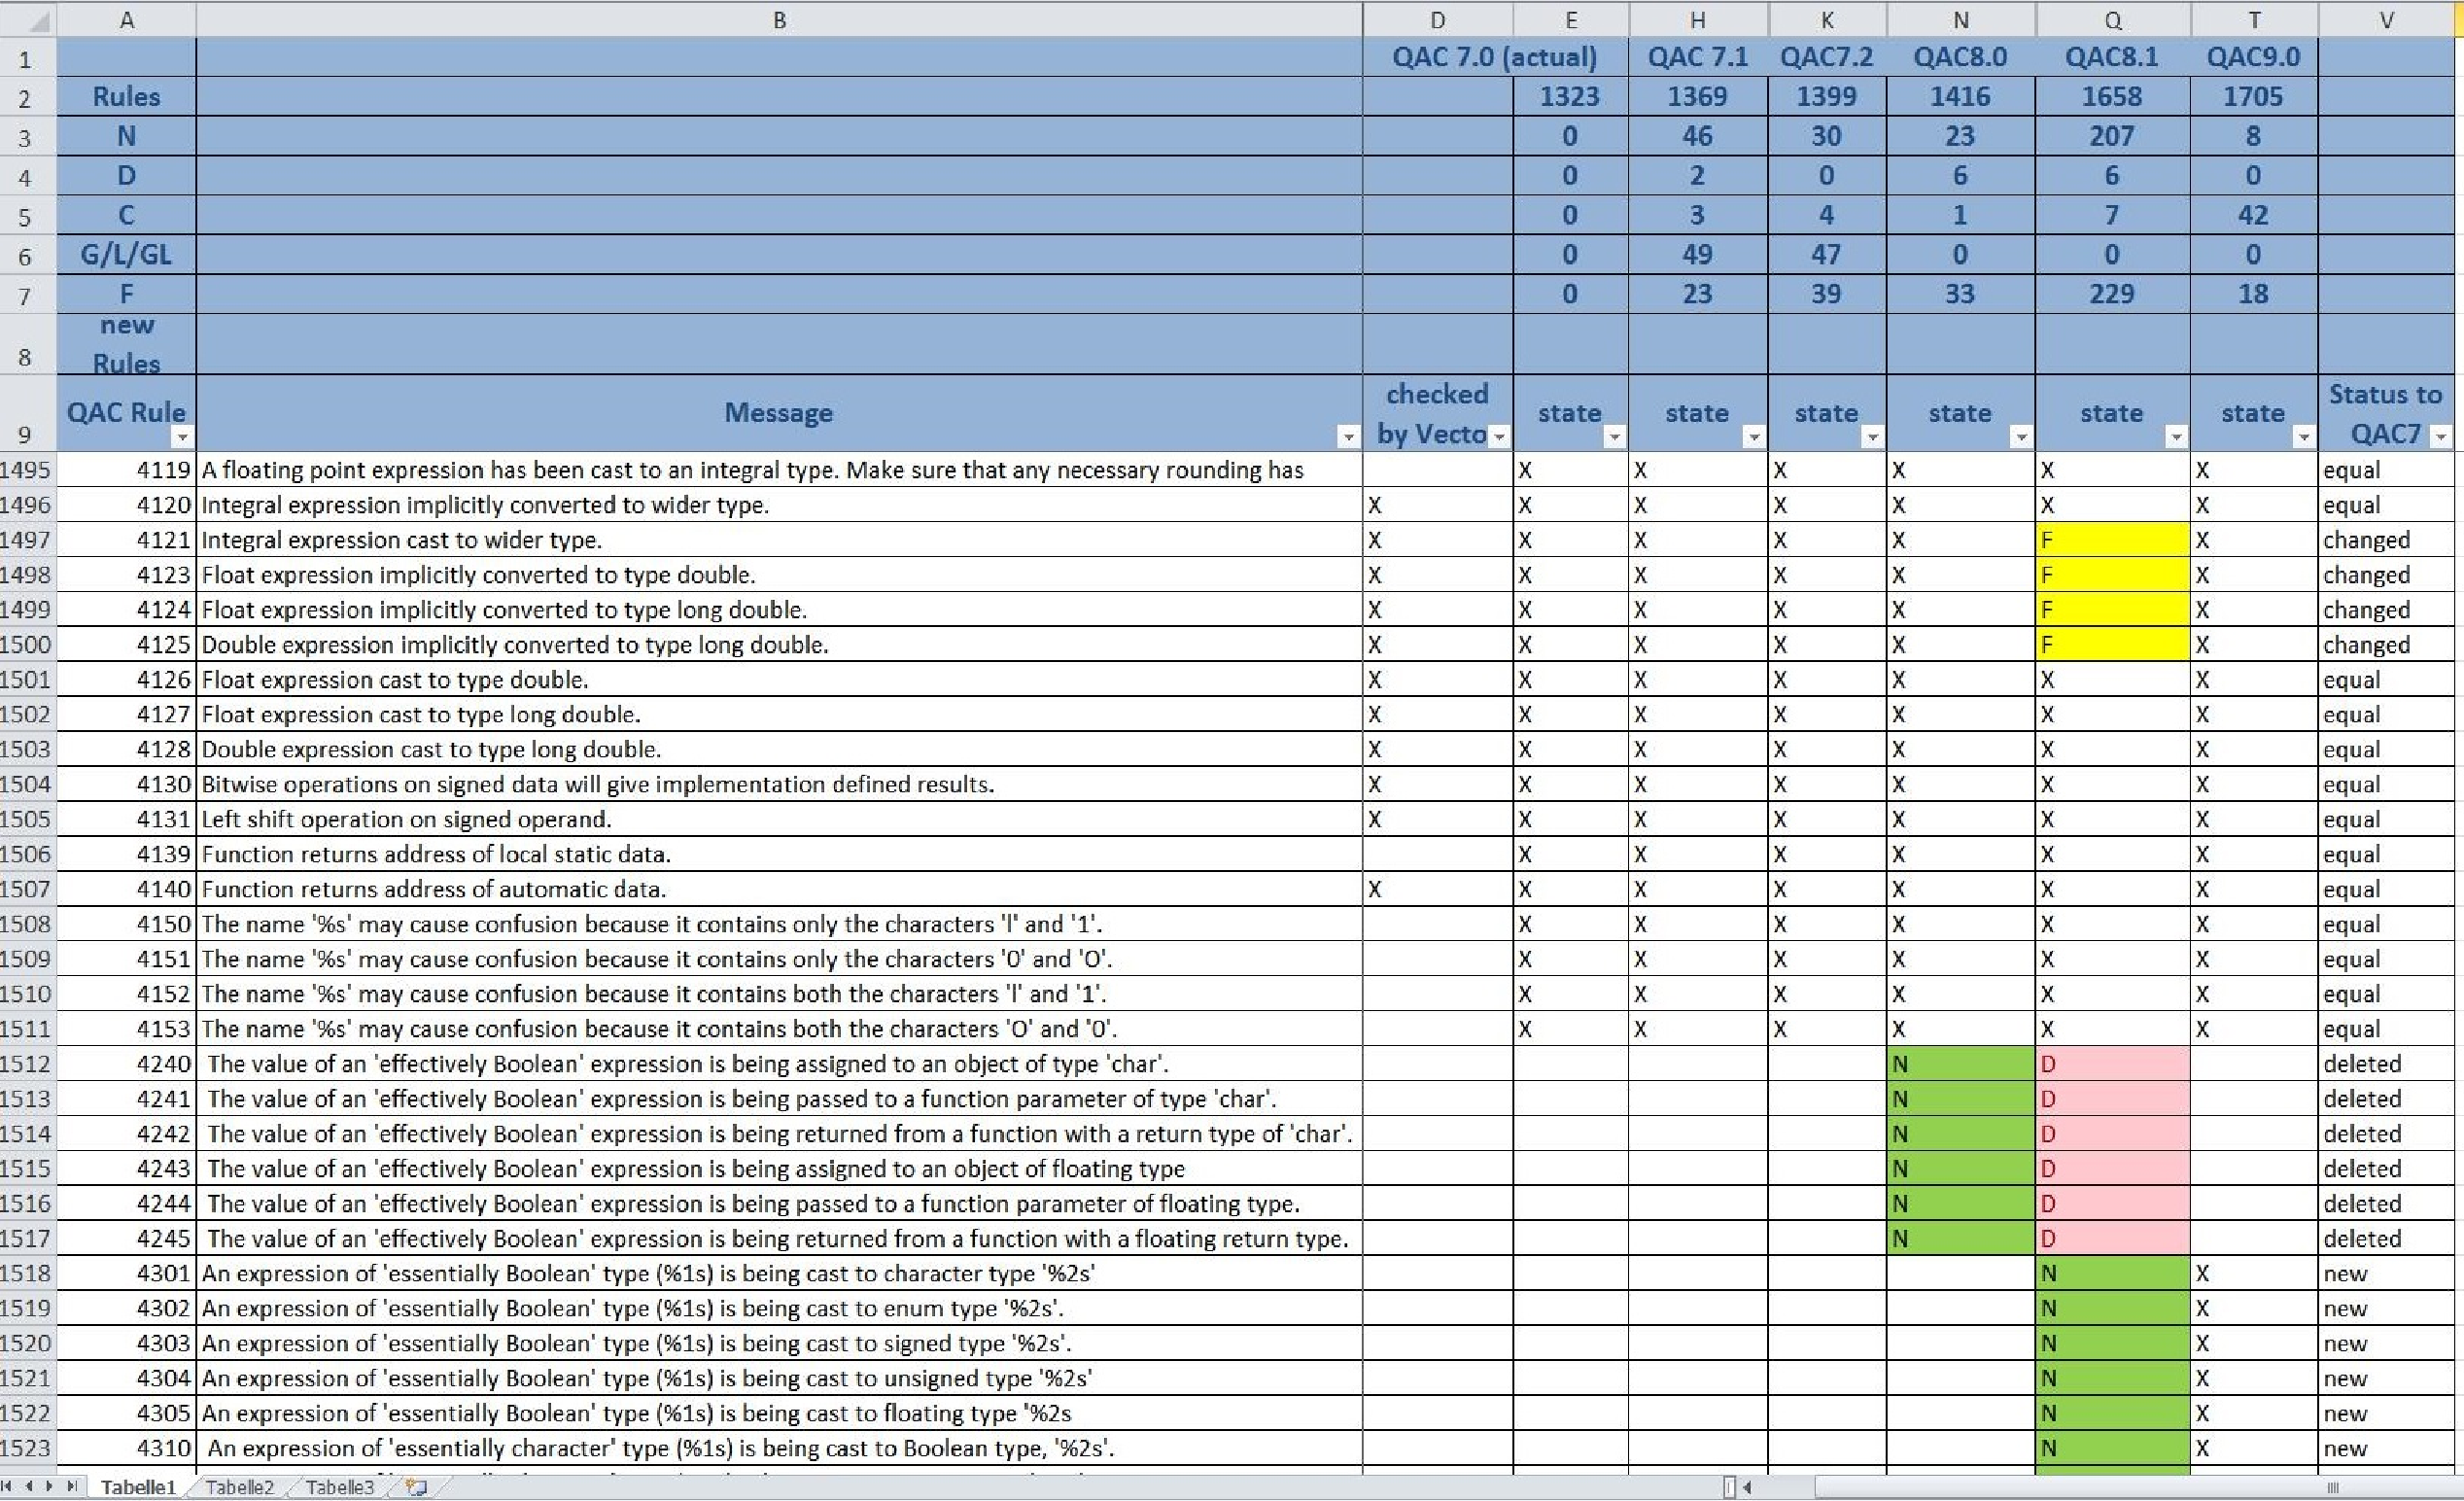
\includegraphics[scale=0.55]{./Bilder/QAC7_9Zusam.pdf}
\caption{Diese Tabelle beschreibt die erste Analyse �ber die �nderungen bei den vom QA-C-Analysetool gepr�ften Regeln, welche sich auf die MISRA-Standards beziehen.}
\label{fig:QAC7_9Zusam}
\end{figure}
\end{landscape}
%

Dabei ist auf der linken Seite des Bilds zu erkennen, dass eine Vielzahl von QA-C zugeh�rigen Regeln aufgezeichnet sind. Insgesamt konnte man 6150 QA-C-Nachrichten und deren entsprechende Eigenschaften zusammenfassen.

Folgende sind die Bewertungskriterien:
%
\begin{itemize}
\item \textbf{N:} New functionality has been introduced.
\item \textbf{F:} A fix of a bug or problem feature. 
\item \textbf{C:} A significant change has been implemented to existing behaviour.
\item \textbf{G/L/GL:} Messages realocated to a different message group or level.
\end{itemize}
%

In der V-Spalte der gezeigten Tabelle wird in Abh�ngigkeit der  modifizierten Versionen angegeben, ob die Eigenschaften der QA-C-Regel im Bezug auf die 7.0 Version gleich geblieben sind, sich ge�ndert haben oder vielmehr neu hinzu gekommen sind. Letzteres kann man sich am Beispiel der QA-C Nachricht 4303 dadurch klar machen, dass diese Nachricht erst in der Version 8.1 eingef�hrt worden ist. Ab dann hat sie bis einschlie�lich der Version 9.0 keine �nderung erfahren. Im Gegensatz dazu gibt es neben der Nachricht 4242 eine Vielzahl von QA-C-Nachrichten, die in der Version 8.1 neu eingef�hrt wurden und in den weiteren \textit{release notes} �nderungen (z.B. gel�scht) erfahren haben. 

Letztere Zusammenh�nge sind bei der Bewertung, inwiefern sich der erw�hnte automatisierte Umstieg bei der MISRA-Pr�fung erm�glichen l�sst, von hoher Bedeutung. Man kann n�mlich ausgehend von der Anzahl an ver�nderten bzw. neuen Nachrichten einsch�tzen, wie hoch der dabei erforderliche Aufwand ist.

\begin{longtable}{|l|l|}
\hline
\textbf{Eigenschaft der Regel} & \textbf{Anzahl an betroffenen Regeln} \\
\endhead
\hline
Gel�scht & 14 \\
\hline
neu eingef�hrt & 390\\
\hline
ge�ndert(einschlie�lich C/F/G/L/GL) & 356\\
\hline
\caption{Diese Tabelle beschreibt die Zusammenfassung der gefundenen Unterschiede bzw. �nderungen bei den vom QA-C-Analysetool gepr�ften Regeln, welche sich auf die MISRA-Standards beziehen.}
\label{tab:TabQAC7_9}
\end{longtable}

\tabvref{tab:TabQAC7_9} stellt besipielhaft wichtige Bewertungskriterien dar, um eine plausible Aussage �ber den angestrebten automatisierten Umstieg der betrachteten MISRA-Analysen geben zu k�nnen. 

In erster Linie sind im Laufe der Versionen eine hohe Anzahl an neuen gepr�ften QA-C-Nachrichten eingef�hrt worden. Auf der anderen Seite gibt es sehr viele Nachrichten, deren Struktur ge�ndert oder angepasst worden sind. Wird ein Entwicklungsprojekt mit der Version 9.0 des QA-C-Analysetools gepr�ft, dann ist mit hoher Wahrscheinlichkeit zu erwarten, dass dabei eine hohe Anzahl an Warnungen angezeigt werden. Die entsprechenden Stellen im Code, auf welche sich die Warnungen beziehen, m�ssten nachtr�glich  dementsprechend h�ndisch einzeln angepasst\footnote{Die entsprechenden \glqq deviations\grqq~im Code m�ssten durch plausiblen \glqq justifications\grqq~begr�ndet werden.} werden.
\newpage
%
\section*{F�nfte Woche}\label{sec:VierteWoche}
%
Beim letzten Teil der ersten Aufgabestellung ginge es darum eine Vielzahl von Basissoftware-Modulen sowohl mit QA-C 7.0 als auch QA-C 9.0 zu analysieren. Ziel dieser Teilaufgabe ist es, eine Voruntersuchung zur Integration von QA-C9\footnote{QA-C9 weist auf die Version 9.0 des betrachteten Analysewerkzeugs hin} in die bestehende Entwicklungsinfrastruktur durchzuf�hren.

Vor der Beschreibung der genannten QA-C-Analysen wird auf die Einstellungen eines QA-C9-Projekts eingegangen.
%
\paragraph*{Bestandteile und wichtige Einstellungen eines QA-C9-Projekts}
%
Erst dieses Jahr ver�ffentlichte QA-Systems die genannte QA-C9-Version. Aus diesem Grund konnte die Voruntersuchung nur mithilfe einer Testlizenz stattfinden.

Die Dokumentation, welche von QA-Systems zur Verf�gung gestellt wird, sollte zur richtigen Verwendung des Tools genau analysiert werden. Im Vergleich zu den \textit{personality files}, die bei QA-C7 verwendet wurden, �hnliche Files in QA-C9 erstellt werden, um ein Projekt einzustellen. 

Analog zum Unterkapitel \ref{QAC7Einf} werden im Folgenden die Einstellungsfiles eines QA-C9 Projekts zusammenfassend eingef�hrt:

\begin{itemize}\label{it:ConfFileQA9}
\item Analysis Configuration File (ACF): \\
definiert die Analyse-Einstellungen, die projektabh�ngig sind wie Include-Pfade, projektabh�nigie Defines, usw.
\item  Rule Configuration File (RCF): \\
Einstellungen bez�glich der f�r die Untersuchung relevanten QA-C-Nachrichten.
\item Compiler Compatibility Templates (CCT): \\
definiert die Einstellungen f�r den Compiler, der bei der Entwicklung der Source Files verwendet wird. 
\item Project Definition File (prqaproject.xml): \\
Hierbei werden u.a. die Pfade der zu analysierenden Files angegeben.
\end{itemize}

Mit der QA-C9-Version ist es m�glich �ber die vorhandene Benutzeroberfl�che (siehe \figvref{fig:QAC9_GUI}) die Einstellungen vorzunehmen oder ebenfalls dadurch, dass man die oben genannten Files entsprechend bearbeitet. Abbildung \ref{fig:QAC9_GUI} zeigt die GUI der aktuellen QA-C9-Version, die im Vergleich zur QA-C7-Version benutzerfreunlicher gestaltet ist.
%
\begin{figure}[!htp]
\centering
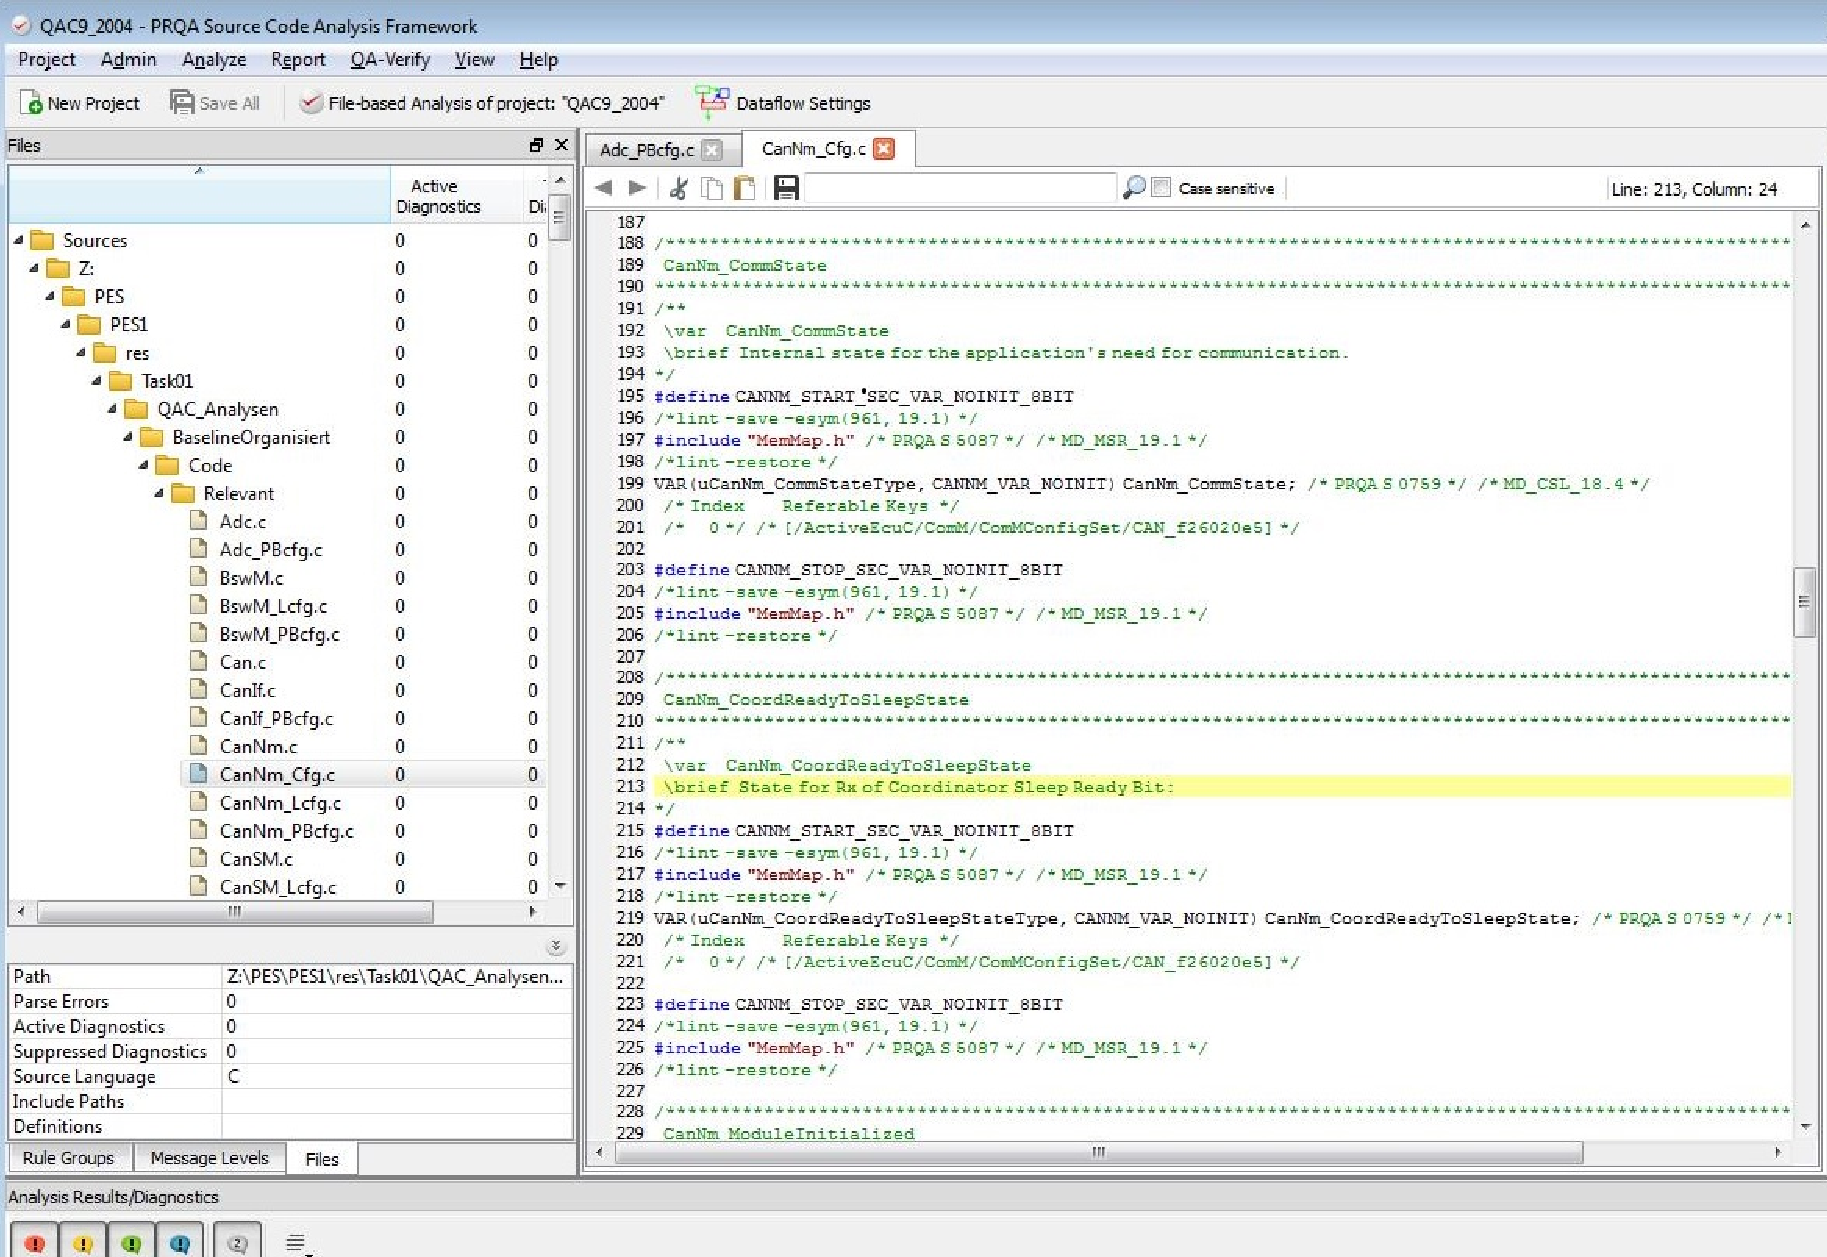
\includegraphics[scale=0.5]{./Bilder/QAC9_GUI.pdf}
\caption{Benutzeroberfl�che der QA-C9-Software. Diese GUI ist im Vergleich zu der QA-C7-Version benutzerfreundlicher gestaltet.}
\label{fig:QAC9_GUI}
\end{figure}
%
\paragraph*{Ergebnisse einer statischen Analyse mithilfe von QA-C9}
%
Um sich mit QA-C9 vertraut zu machen, lohnt es sich, mit der Analyse f�r die bereits im Unterkapitel \ref{QAC7Einf} behandelte \textit{simple component} klein anzufangen.

Nachdem das QA-C9-Projekt �ber die GUI eingestellt wurde, war es m�glich entsprechende Reports zu erstellen. Die Reports k�nnen direkt als HTML-Files ausgegeben werden und Hinweise, ob bei der Analyse Findings aufgetretten sind, sind aus bestimmten Stellen in der GUI abzulesen.

Der wesentliche Unterschied zwischen den QA-C7- und QA-C9-Versionen besteht darin, dass in der QA-C7-Version die Report-Findings bei einem bestimmten Header File sich in der gesammten Analyse ausbreiten. Dies geschieht, wenn diese Files in anderen Files eingebunden werden. Leider lassen sich die Findings eines bestimmten Files schlecht von diesen genannten Findings unterscheiden. Dies ist bei der QA-C9-Version nicht der Fall, denn dabei werden die Findings von eingebundenen Header-Files isoliert behandelt und gehen nicht in den Report anderer Files ein.

Die Ergebnisse der Analyse mit der Version 7.0 wurden zusammen mit den oben genannten Ergebnissen der Reports verglichen und sind in \figvref{fig:QACSimpleComp} mittels einer Tabelle dargestellt.

Auf der linken Seite der Abbildung sind die analysierten Files dargestellt. Die Ergebnisse sind nach den verwendeten Versionen sortiert. Eine solche Darstellung kann hilfreich sein, um beipielsweise Nachrichten aufzuzeichnen, die bei einem bestimmten analysierten File in einer Version jedoch nicht in der anderen erkannt werden. Das ist der Fall beispielsweise bei der Nachricht 841, die in allen Files bei der Version 7.0 jedoch in keiner der folgenden Versionen erkannt wird. 
%
\begin{figure}[!ht]
\centering
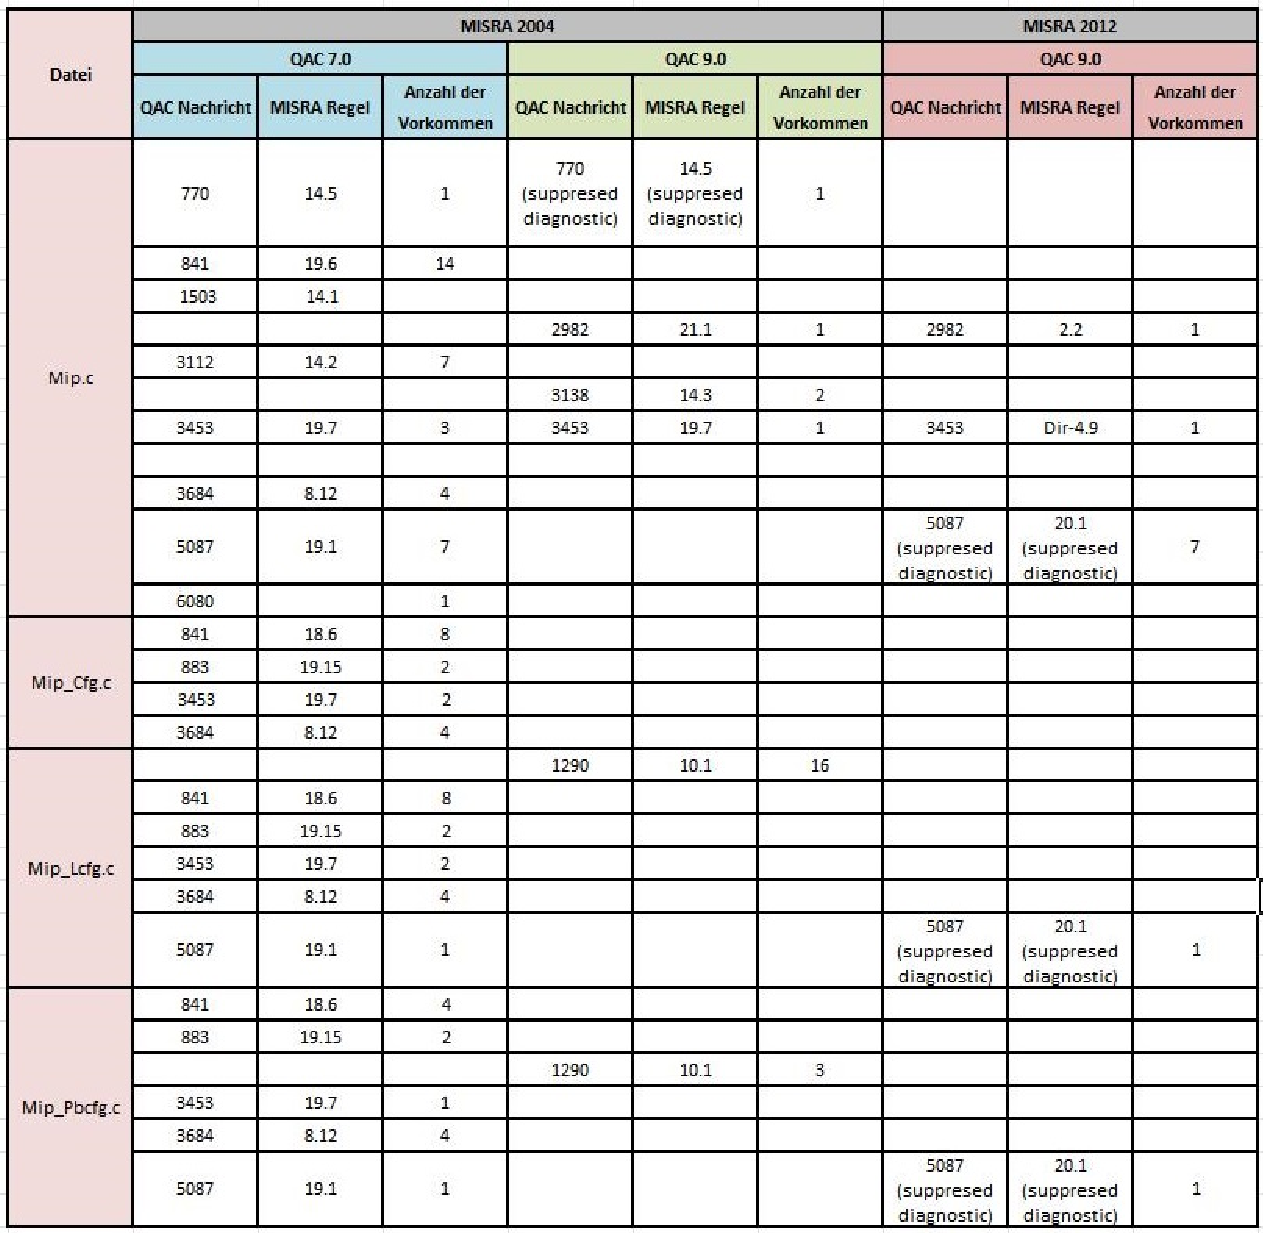
\includegraphics[scale=0.7]{./Bilder/QACSimpleComp.pdf}
\caption{Ergebnisse einer statischen Codeanalyse, die bez�glich einer \textit{simple component} mithilfe der QA-C7- und QA-C9-Versionen durchgef�hrt wurde. Auf der linken Seite der Abbildung sind die analysierten Files dargestellt. Die Ergebnisse sind nach den verwendeten Versionen sortiert.}
\label{fig:QACSimpleComp}
\end{figure}
%

Drauf aufbauend sollte ein umfangreicheres QA-C9-Projekt zur statischen Codeanalyse einer gr��eren Anzahl an BSW-Files eingestellt werden. In diesem Fall w�rde sich die Einstellung eines solchen Projekts als sehr umst�ndlich erweisen, wenn dies h�ndisch durchgef�hrt wird. Dies liegt daran, dass die Quelldateien sich normalerweise in mehreren Unterordner organisiert befinden und die jeweiligen Pfade angegeben werden m�ssen. Letzteres betrifft sowohl die Eingabe der Einstellungsfiles �ber die GUI als auch die manuelle Bearbeitung der Einstellungsfiles ACF, RCF, CCT sowie der XML-Project-Definition-Datei. 
%
\newpage
\section*{Sechste Woche}
%
Bei einer solchen gro�en Anzahl an zu analysierenden Files, die in der Regel sehr oft bei einem Entwicklungsprojekt vorkommen, sollte eine automatisierte Generierung von Analysereports m�glich sein. Hierbei k�nnte die Verwendung einer Skriptsprache wie PERL oder Phyton Abhilfe schaffen. Letztere erleichtern u.a. den automatisierten Umgang mit Textdateien und Verzeichnissen.

Da bisher in der Abteilung einige Mitarbeiter bei der Programmierung mit PERL gro�e Erfahrung gesammelt haben, entschloss ich mich diese Programmiersprache zur Bearbeitung der Konfigurationsdateien einzusetzen. Eine kostenlose IDE, mit der es m�glich ist, \verb|PERL|-Skripte zu erstellen, kompilieren und Debuggen ist nicht leicht zu finden. Eine gute Alternative bietet die in Abbildung \ref{fig:EPICskr1} gezeigte EPIC-IDE \cite{EPICIDE}. Diese steht als Eclipse-Plugin kostenlos zur Verf�gung und stellt nicht nur die M�glichkeit dar, \verb|PERL|-Skripte zu bearbeiten, sondern auch diese zu kompilieren und mit einem integrierten Tool zu debuggen. Au�erdem ist diese sehr bekannt, wobei das Support ausreichend in Foren zu finden ist.

Bei der Installation und Inbetriebnahme dieser \verb|PERL|-IDE muss man auf bestimmte Fehlermeldungen achten, die sich meistens auf die Version des verwendeten \verb|PERL|-Kompilers beziehen. Um diese zu beheben, ist man auf Internetrecherche angewiesen.

Um die genannten Files von den unterschiedlichen Verzeichnissen in ein einzelnes Verzeichnis zu �bertragen, wurde \lstref{lst:PERL_Dateiueb} erstellt.
%
\begin{figure}[!ht]
\centering
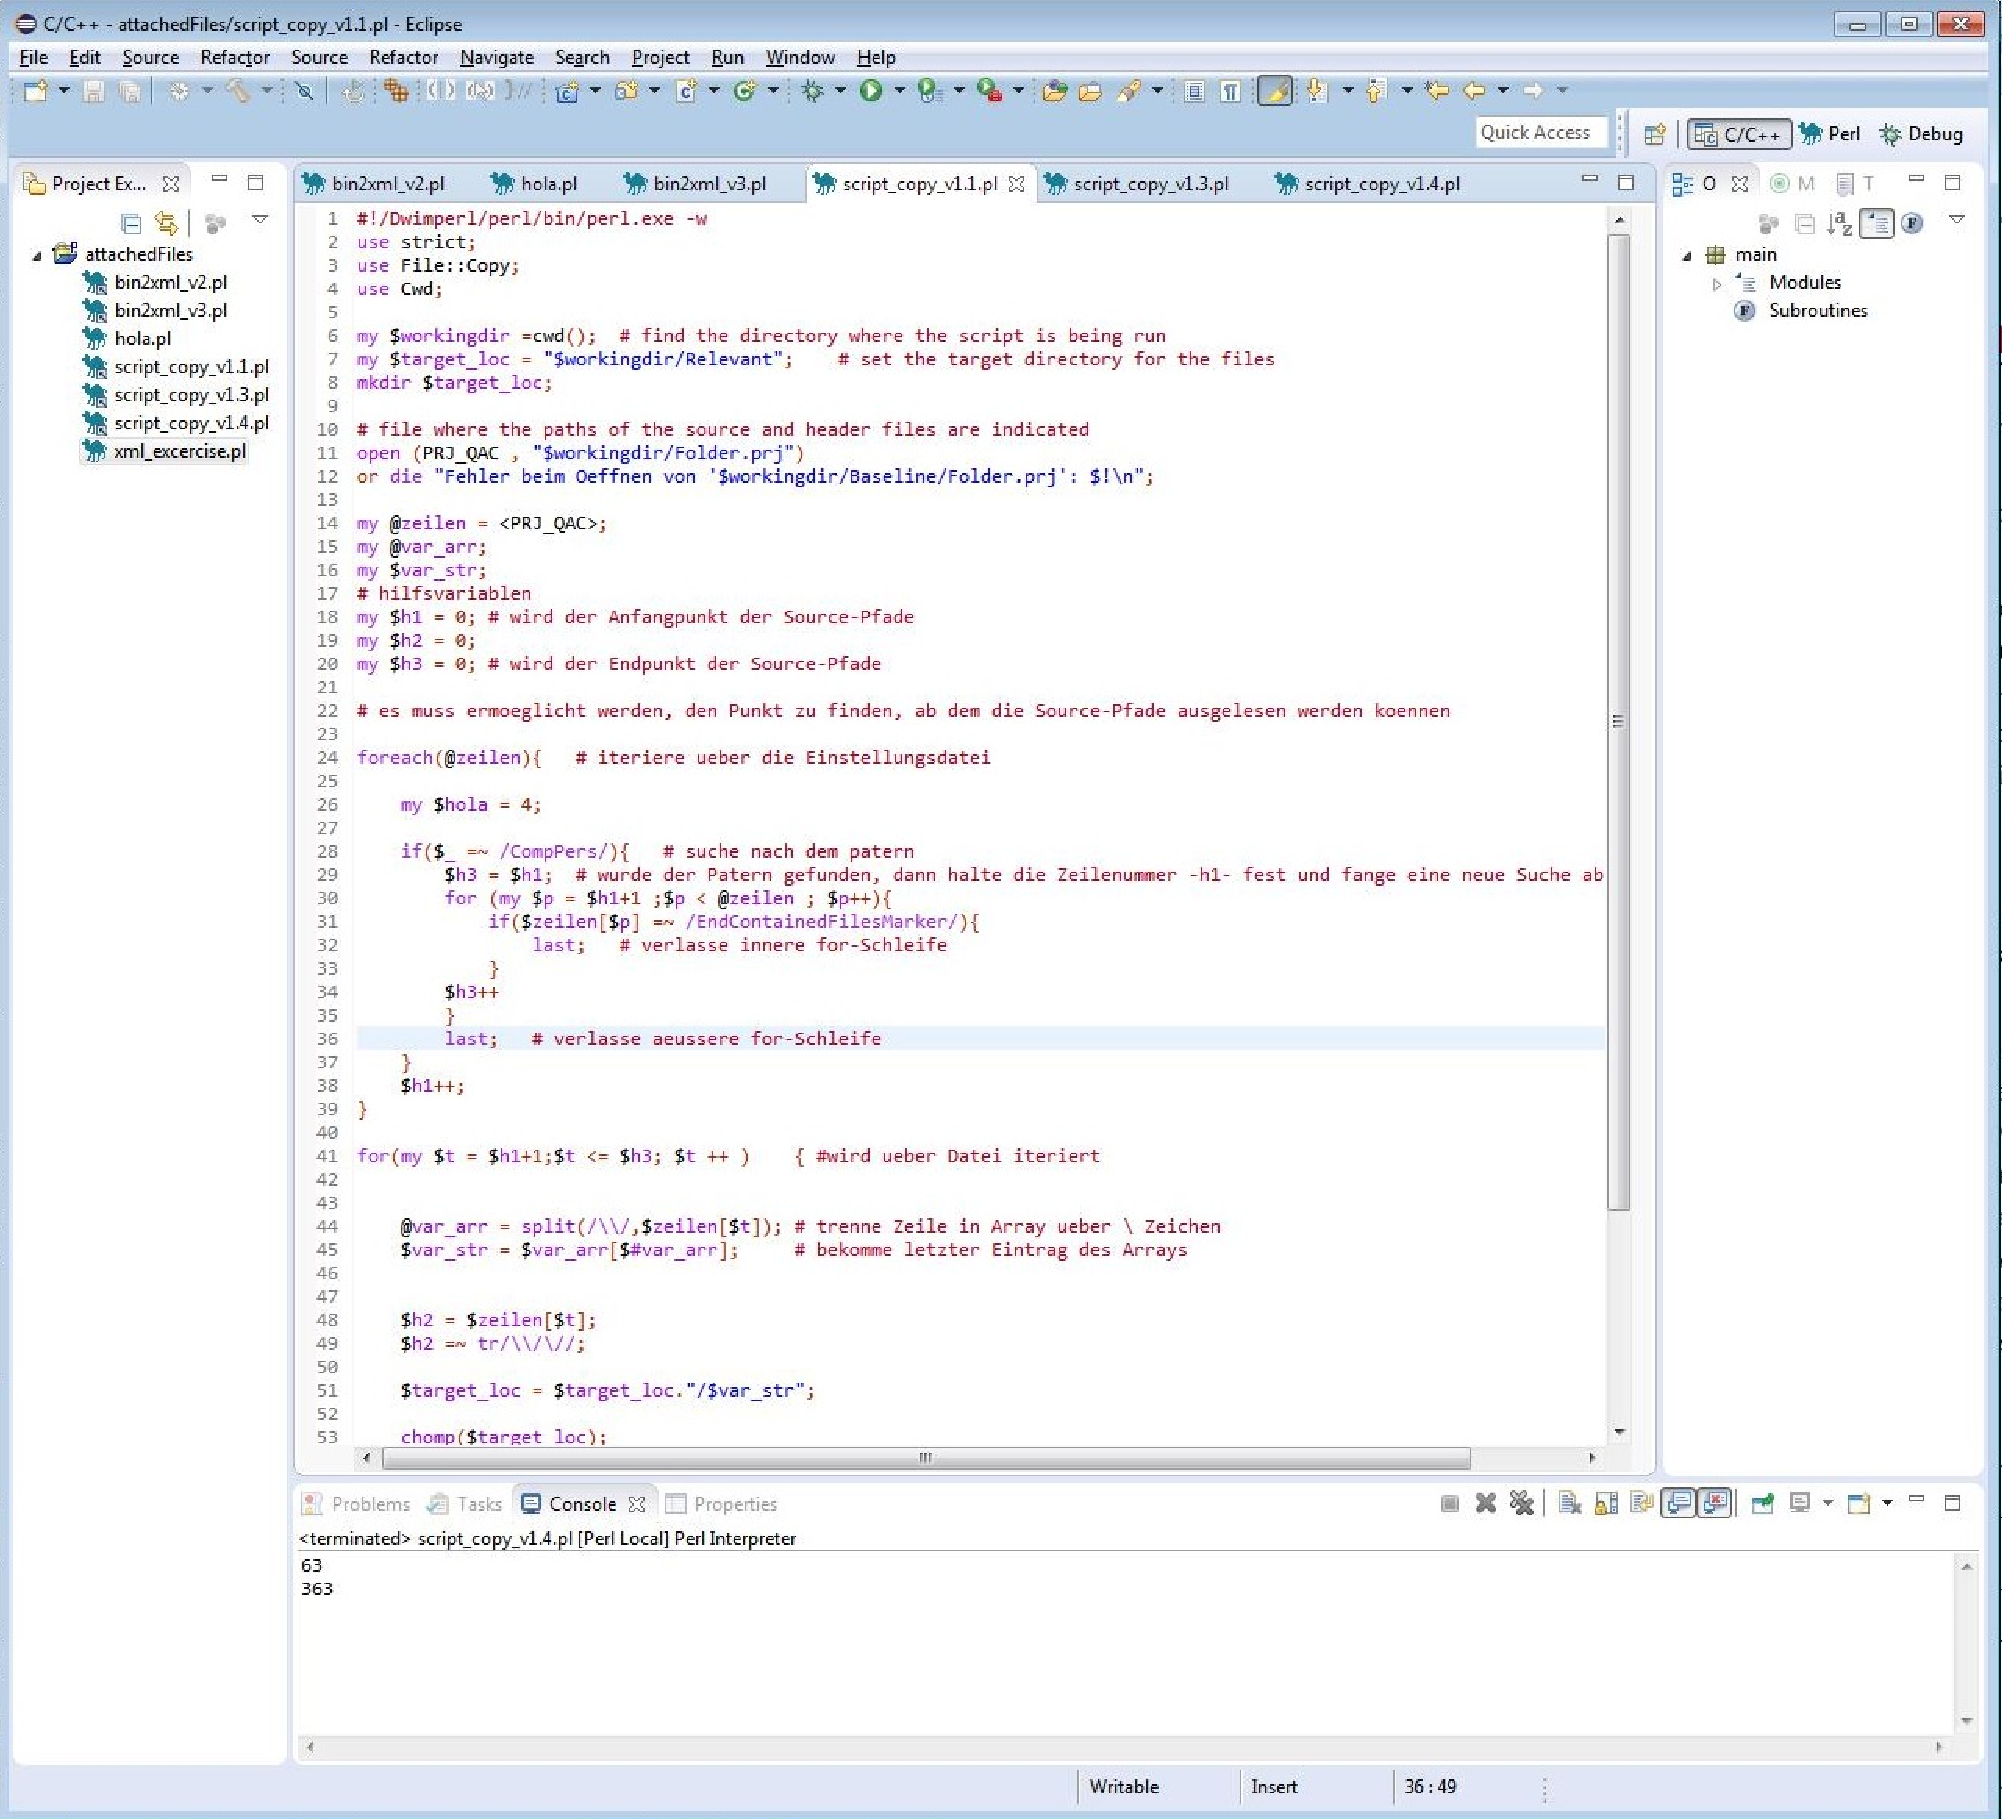
\includegraphics[scale=0.6]{./Bilder/EPIC_skr1.pdf}
\caption{Eclipse-Benutzeroberfl�che bei Anwendung der \texttt{PERL}-IDE.}
\label{fig:EPICskr1}
\end{figure}

Die �bertragung der Dateien war nicht die einzige Aufgabe, die zum Erstellen des QA-C9-Projektes durchgef�hrt werden musste. Es war au�erdem notwendig die Pfade der einzelnen zu analysierenden Dateien anzugeben. Wie weiter oben in diesem Kapitel erl�utert, bedient sich QA-C9 einer XML-Konfigurationsdatei, um dabei sowohl die Pfade der zu analysierenden Dateien als auch weitere wichtige Einstellungen festzulegen.

Diese XML-Datei als Textdatei so zu bearbeiten, dass dabei die richtige Eintr�ge hinzugef�gt werden, ist sehr hilfreich, um eine automatisierte statische Codeanalyse von sehr vielen Sourcefiles durchzuf�hren. Dies ist das Ziel, um im Nachhinein die ganze statische Codeananalyse lediglich durch den Aufruf der richtigen Befehle �ber eine Kommandozeile ausf�hren zu k�nnen.
Dazu wird ein von QA-Systems zur Verf�gung gestellte Compiler mit den richtigen Optionen aufgerufen, wobei dem Compiler auch die richtigen QA-C9-Konfigurationsdateien zur Verf�gung stehen m�ssen. Diese Methode hat man zwar bisher in der Abteilung eingesetzt, der dabei verwendeter Compiler geh�rt zu der QA-C7-Version \cite{MISRACodeMetric}.

Da die Version QA-C9 einen �hnlichen Compiler (QA-CLI) zur automatischen Ansteuerung einer statischen Codeanalyse bietet, ist es hilfreich, sich die dazu n�tigen Compiler-Optionen anzuschauen und auszusuchen. Eine genaue Beschreibung der dabei relevanten Compilerbefehle bez�glich der QA-C9-Version k�nnen in \cite{PRQA9}~nachgelesen werden.

Damit die erw�hnten Konfigurationsfiles dem QA-CLI-Compiler zur Verf�gung stehen, m�ssen diese erstmal mit den richtigen Informationen aufbereitet werden. Dadurch w�rde sich die automatisierte statische Codeanalyse �ber Compiler-Aufrufe bzw. �ber einen Batch-Skript auszuf�hren lassen.

Um die Aufbereitung der Einstellungsfiles habe ich ebenfalls die bei der Programmierung des ersten \verb|PERL|-Skripts erworbenen Kenntnisse genutzt. In dieser zweiten Anwendung bearbeitet ein neuer \verb|PERL|-Skript ein vorhandenes Template-File eines QA-C9-Projekts, welches nur wenige Eintr�ge enth�lt. Dann werden die relevanten, zu analysierenden Files und deren Pfadenamen hinzugef�gt. Das Ergebnis nach der Ausf�hrung des in \lstref{lst:PERL_XML} angegebenen \verb|PERL|-Skripts kann im folgenden Listing betrachtet werden. Zu erw�hnen ist, dass dies nur ein kleiner Ausschnitt der gesamten Eintr�ge ist.
%
\definecolor{forestgreen}{RGB}{34,139,34}%definition fuer xml Comment style 
\begin{lstlisting}[language=XML, caption = {Project Definition File (prqaproject.xml) bez�glich der QAC-9-Version}, label={lst:QAC9_xml}]
...
 <!-- Files in project... -->
 <files>
  <!-- Explicit files... -->
  <file target="C" name="Adc.c" folder="=Z:/PES/PES1/res/Task01/QAC_Analysen/Relevant"/>
  <file target="C" name="BswM.c" folder="=Z:/PES/PES1/res/Task01/QAC_Analysen/Relevant"/>
  <file target="C" name="Can.c" folder="=Z:/PES/PES1/res/Task01/QAC_Analysen/Relevant"/>
  <file target="C" name="Can_Irq.c" folder="=Z:/PES/PES1/res/Task01/QAC_Analysen/Relevant"/>
  <file target="C" name="CanIf.c" folder="=Z:/PES/PES1/res/Task01/QAC_Analysen/Relevant"/>
  <file target="C" name="CanNm.c" folder="=Z:/PES/PES1/res/Task01/QAC_Analysen/Relevant"/>
  <file target="C" name="CanSM.c" folder="=Z:/PES/PES1/res/Task01/QAC_Analysen/Relevant"/>
  <file target="C" name="CanTp.c" folder="=Z:/PES/PES1/res/Task01/QAC_Analysen/Relevant"/>
  <file target="C" name="CanTrcv_30_GenericCan.c" folder="=Z:/PES/PES1/res/Task01/QAC_Analysen/Relevant"/>
  <file target="C" name="CanTSyn.c" folder="=Z:/PES/PES1/res/Task01/QAC_Analysen/Relevant"/>
  <file target="C" name="CanXcp.c" folder="=Z:/PES/PES1/res/Task01/QAC_Analysen/Relevant"/>
  <file target="C" name="Com.c" folder="=Z:/PES/PES1/res/Task01/QAC_Analysen/Relevant"/>
  <file target="C" name="ComM.c" folder="=Z:/PES/PES1/res/Task01/QAC_Analysen/Relevant"/>
  <file target="C" name="Crc.c" folder="=Z:/PES/PES1/res/Task01/QAC_Analysen/Relevant"/>
  <file target="C" name="Cry.c" folder="=Z:/PES/PES1/res/Task01/QAC_Analysen/Relevant"/>  
...
\end{lstlisting}
%
Dabei ist ersichtlich, wie die Namen der zu analysierenden Files und die Pfade anzugeben sind, wo sich dieselben befinden. Dies h�ndisch bzw. per Maus-Klick �ber die GUI einzutragen w�re sehr m�hsam, was auf die Notwendigkeit der automatisierten Handhabung dieser Einstellungen hinweist.
%
\section{Ergebnisse der 1. Aufgabenstellung}
%
Eine erste detaillierte Analyse �ber die Kompatibilit�t zwischen den beiden MISRA Versionen (2004 bzw. 2012) wurde durchgef�hrt. Es wurde festgestellt, dass von der britischen \glqq The Motor Industry Sofrware Reliability Association\grqq~bereits ein Dokument ver�ffentlicht wurde, welches die �nderungen und Gemeinsamkeiten zwischen den genannten Versionen aufzeichnet. Dieses Dokument kann als Grundlage dienen, um handische Vergleiche zwischen den beiden Versionen durchzuf�hren.

Au�erdem wurde eine Analyse zwischen der aktuell von Vector eingesetzten QA-C7- und der letzten QA-C9-Version des statischen Analysetools. Dabei war das Ziel die im Laufe der Zeit bez�glich der neuen Version eingef�hrten �nderungen festzulegen. 

In beiden F�llen wurde festgelegt, dass Regeln sowohl gel�scht als auch neu eingef�hrt wurden. Umganreiche �nderungen in der Struktur vieler gepr�ften MISRA- bzw. QA-C-Regeln sind eingef�hrt worden. Dies weist auf eine nicht zu vernachl�ssigende Wahrscheinlichkeit hin, dass bei einer statischen Codeanalyse von bestehenden Software-Komponenten mit der neuen QA-C-Version eine Vielzahl an Warnungen gemeldet werden. Der alysierte Code kann somit bez�glich der neuen MISRA-Regeln mit einem hohen Aufwand so angepasst werden, dass diese Abweichungen nicht mehr auftretten.

Anschlie�end wurden zwei M�glichkeiten vorgestellt, um ein Projekt mit der neuen QA-C9-Version des statischen Analysetools aufzustellen. Es wurden dabei zwei \verb|PERL|-Skripte programmiert, um einerseits zahlreiche Files von einem Verzeichnis in einen anderes zu �bertragen, ohne dies h�ndisch durchf�hren zu m�ssen. Andererseits l�sst sich mit dem zweiten Skript ein XML-Templatefile (Project Definition File) bearbeiten, welches f�r eine automatisierte statische Codeanalyse n�tig ist. Im Gegensatz dazu wird diese Art der Verarbeitung von Text-Files in der Abteilung �ber Batch-Skripts und andere programmiersprachen durchgef�hrt.
%
\newpage
\section*{Siebte Woche}
%
In der siebten Woche wurde mir die 2. Aufgabestellung vorgestellt. Dabei ginge es darum, mich umfassend mit einem Basic Test Environment (BTE) zu besch�ftigen, welches in der PES Abteilung entwickelt wurde. Ich musste mich mit dem Tool vertraut machen und seine Funktionsweise verstehen, um es anschliessend um weitere Funtionalit�ten zu erweitern.
%
\section{Zweite Aufgabenstellung}
% 
Wie oben erw�hnt war es notwendig die wichtigsten Eigenschaften und Besonderheiten vom BTE-Tool zusammenzufassen und kennenzulernen. Anhand dieser Analyse wird es klarer, an welcher Stelle die Funktionalit�ten zu erg�nzen sind.
%
\subsubsection*{BTE - Basic Test Environment}
%
Das BTE ist ein in \verb|C| implementiertes Component-Unit-Test-Framework, mit dessen Hilfe man in der Abteilung hardwareunabh�ngige (AUTOSAR-) BSW-Komponeneten testet \cite{BTE}.

Die in Abbildung \ref{fig:BTE_func1} vorgestellte BTE-Version bietet verschiedene Testsfunktionalit�ten, u.a. das Nachbilden (emulation) einer inneren ECU-Umgebung, die Ereignisprotokollierung und das Erstellen von entsprechenden Reports \cite{BTE}. 
%
\begin{figure}[!htp]
\centering
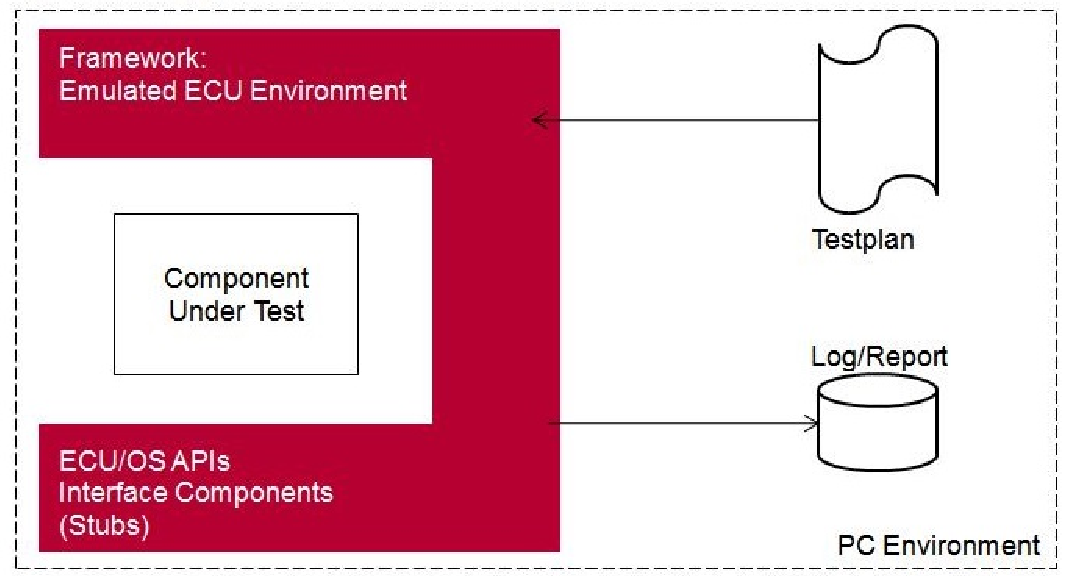
\includegraphics[scale=0.8]{./Bilder/BTE_func1.pdf}
\caption{Framework-Emulation of ECU environment on a PC. Entnommen aus \cite{BTE}.}
\label{fig:BTE_func1}
\end{figure}
%

Im Diagram wird durch die rote Box die Nachbildung der inneren ECU-Umgebung gezeigt. Diese Box besteht aus mehreren Platzhaltern, sogenannten Stubs, die Komponenten simulieren/ersetzen. Dabei ist ersichtlich, dass der Testplan sowohl die simulierten Stubs als auch die Component Under Test (CUT) steuert, damit vom Framework einen entsprechenden Log/Report ausgegeben wird. Aufgrund der stubbasierten Funktionsweise des vorgestellten Frameworks, ist es nicht n�tig die gesammte Komponenten, die in einem Stuerger�t vorkommen, zu betrachten. Dies ist ein gro�er Vorteil.

Das Klassendiagram, welches in Abbildung \ref{fig:BTELogListold} gezeigt wird, gibt einen Teil der existierenden BTE-Struktur wieder. Das Teilmodul \verb+TestHandler+ steuert den Ablauf der Testdurchf�hrung, wobei nur �ber das Modul \verb+BteReport+ auf die Testreport-Datei zugegriffen wird, um diese zu bearbeiten. Die Funktionalit�t \verb+BteCheckX+ bezeichnet bestimmmte Komponenten der BTE, die wie das Modul \verb+BteReport+ direkt auf den VTR-Report zugreifen, um beispielsweise bestimmte Meldungen auszugeben. Die dabei verwendete Methodesaufrufe werden nicht als solche zu testende Methodensaufrufe von der BTE registriert. 
%
\begin{figure}[!htp]
\centering
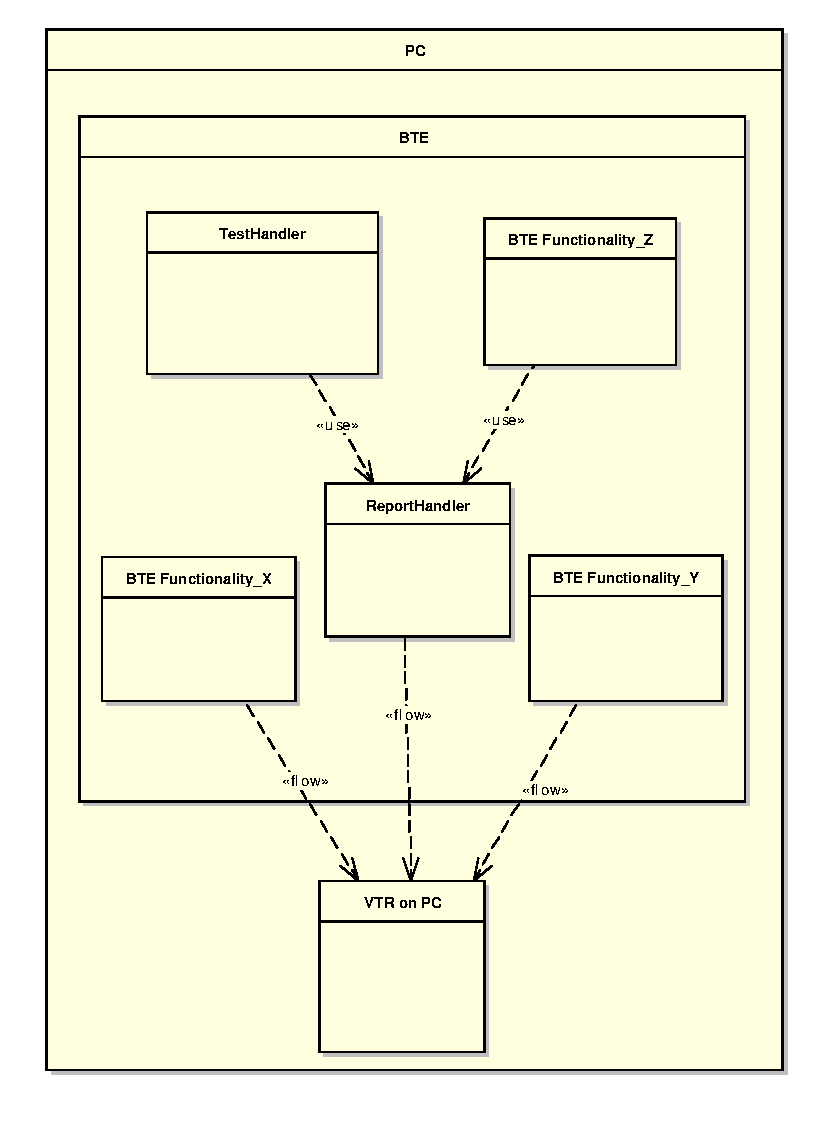
\includegraphics[scale=0.75]{./Bilder/BTELogListold_cropped.pdf}
\caption{Klassendiagramm zur Erg�nzung der Softwarespezifikation des erweiterten BTE-Tools. Dabei k�nnen die funktionalen Zusammenh�nge zwischen den ursprunglichen Modulen erkannt werden.}
\label{fig:BTELogListold}
\end{figure}
%

Gegen�ber den genannten Funktionalit�ten bzw. Vorteile gibt es bei der Verwendung des BTEs folgenden Nachteil, der sich eher als eine Einschr�nkung �u�ert: Mit dem Tool lassen sich bequem Testreports auf einem lokalen Rechner ausgeben und abspeichern. Dabei werden jedoch betriebssystemabh�ngige Funktionen zum Umgang mit Strings ben�tigt, die in der Regel viele Hardwareresourcen verbrauchen. Die BTE l�sst sich somit nur auf Rechnern sinnvoll einsetzen, die genug Arbeitsspeicher und Speicherplatz zur Verf�gung stellen.

\begin{Aufgabenstellung}
Die Aufgabestellung basiert somit auf folgender Anforderung: Es w�re vorteilhalft, die BTE-Struktur (siehe Abbildung \ref{fig:BTELogListold}) so zu erweitern, dass das Tool ebenfalls auf einem eingebetteten System l�uft. Der Grund daf�r ist, dass es dadurch m�glich w�re, Testreports von BSW-Komponenten unter realen Bedingungen erstellen zu k�nnen. 
\end{Aufgabenstellung}
%
\subsubsection*{Test-Hardware}
%
Eine Test-Hardware, auf der die BTE laufen soll, wurde mir zur Verf�gung gestellt. Es handelte sich dabei um das STM32F4-DiscoveryBoard, auf dem der  Mikrocontroller STM32F407VG (Cortex-M4-Hardwarearchitektur) eingebaut ist. Siehe Abbildung \ref{fig:discovery}.

Um die Aufgabe zu l�sen, war es notwendig das STM32F4-DiscoveryBoard in Betrieb zu nehmen und dabei eine passende Entwicklungsumgebung zu verwenden. Diese sollte dementsprechend geeignete Compiler- und Linker-Bibliotheken zur Verf�gung stellen, die das Erstellen einer Applikation f�r den  Mikrocontroller unterst�tzen. 
%
\begin{figure}[!htp]
\centering
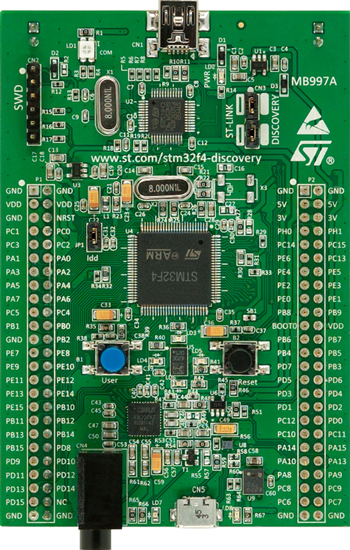
\includegraphics[scale=0.4,angle=90]{./Bilder/stm32f4_discovery.jpg}
\caption{Verwendete Test-Hardware (STM32F4), auf welcher die RT-BTE lauff�hig sein soll.}
\label{fig:discovery}
\end{figure}
%

Da ich in vergangenen Projekten bereits Erfahrung bei der Programmierung des genannten Mikrocontrollers sammeln konnte, entschloss ich mich die Eclipse-IDE und das dabei zur Verf�gung stehende CDT\footnote{C/C++ Development Tooling}-Plugin einzusetzen. Dieses erweitert Eclipse und bietet u.a. die M�glichkeit C/C++ Programme zu editieren, zu kompilieren und zu linken~\cite{EclipseCDT}. 

In ~\cite{EclipseSTM32Youtube} werden weitere, notwendige Tools angegeben, die die Programmierung des Mikrocontrollers erm�glichen:
%
\begin{itemize}
\item GDB Hardware Debugging: ein zus�tzliches Eclipse-Plugin
\item GDB: der GNU Debugger-Programm
\item GDB-Server: stellt eine Verbindung mit GDB und dem JTAG-Interface her.
\item Toolchain: make, Compiler, Linker, GDB, Bibliotheken, usw.
\end{itemize}
%
\newpage
%
\section*{Achte Woche}\label{siebteWoche}
%
\section{Durchf�hrung der zweiten Aufgabenstellung}\label{durchfAuf2}
%
Jedes Software-Projekt basiert auf einer grundlegenden Anforderungsanalyse. Bei der vorliegenden Aufgabe wurde ebenfalls eine Anforderungsanalyse durchgef�hrt, welche im folgenden vorgestellt wird.
%
\subsection*{Anforderungsanalyse}\label{Anforderungen}
%
Die Erweiterung des BTE-Tools soll folgende Anforderungen erf�llen:
%
\begin{enumerate}
\item Urspr�ngliche Implementierungen der BTE-Funktionalit�ten, sollen durch Erweiterungen m�glichst wenig modifiziert werden.
\item Es soll auf einem Embedded-Prozessor lauff�hig sein und mit vorhandenen Hardware-Ressourcen m�glichst sparsam umgehen.
\item Die urspr�ngliche BTE-Funktionalit�ten, einen Test einer Software-Komponente auf einem lokalen Rechner durchzuf�hren und dabei einen passenden Report zu erstellen, sollen immer noch vorhanden sein.
\item Ein Testreport soll bei Verwendung des BTE-Frameworks auf einem eingebetteten System durch eine entsprechende Kodierung auf der RAM des betrachteten Systems abgespeichert werden k�nnen.
\item Eine Funktionalit�t soll vorhanden sein, um aus einer vorgegebenen Bin�rdatei einen Testreport erstellen zu k�nnen. Die Bin�rdatei stellt den RAM-Speicherbereich dar, wo sich der kodierte Testreport befindet.
\item Der aus der Bin�rdatei erstellte Testreport soll dieselbe Struktur eines Testreports haben, der �ber das BTE auf einem lokalen Arbeitsrechner erstellt wird.
\end{enumerate}
%
In Abbildung \ref{fig:BTEUseCase} wird ein Anwendungsfalldiagramm gezeigt, um die funktionalen Anforderungen an dem vorliegenden System besser zu verstehen. 

Dabei ist ersichtlich, dass lediglich der Anwendungsfall \textsf{\textbf{excecute test on embedded device}} die urspr�ngliche BTE-Funktionalit�ten erweitert. Dieser Anwendungsfall beschreibt somit die zu implementierenden Anpassungen und Erweiterungen. Nachdem die Implementierungen der L�sungen zu dieser Aufgabe und dadurch die oben genannten Anforderungen erf�llt werden, hat der Anwender die M�glichkeit, �ber das erweiterte Tool Tests sowohl auf einem lokalen Arbeitsrechner als auch auf einem eingebettenen Prozessor durchzuf�hren. Ein Report kann ebenfalls mithilfe des erweiterten Tools erstellt werden. Im gezeigten Anwendungsfalldiagram ist somit nicht relevant, �ber welchen Weg der entsprechende Testreport erzeugt wird. Dabei ist wesentlich, dass das Tool ebenfalls Reports auf einem eingebetteten System erstellen kann.
%
\begin{figure}[!htp]
\centering
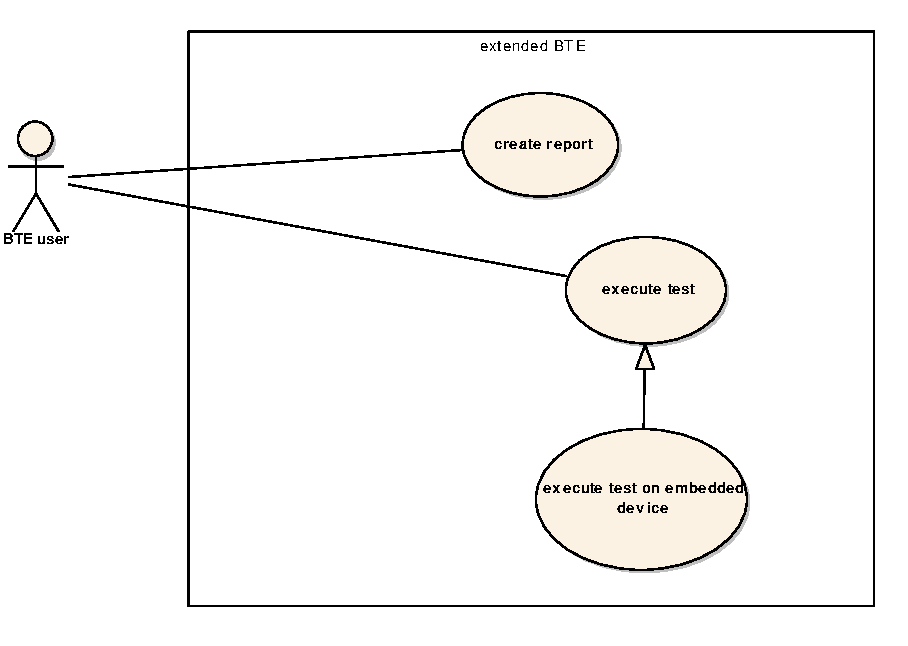
\includegraphics[scale=0.9]{./Bilder/BTEUseCase.pdf}
\caption{Anwendungsfalldiagramm zur Erg�nzung der Softwarespezifikation des erweiterten BTE-Tools.}
\label{fig:BTEUseCase}
\end{figure}%
%
\subsubsection*{Verwendeter L�sungsansatz}\label{Ansaetze}
%
Man muss mit den vorhandenen Hardwareressourcen des eingebetteten Systems, wo die BTE eingebunden werden soll, sparsam umgehen und dabei auch eine Methode einsetzen, bei der beispielsweise der Test-Report direkt auf dem beschr�nkten RAM-Speicher abgelegt wird. Dazu ist es notwendig, eine bestimmte Codierung festzulegen, wie die Daten abzuspeichern sind.

Am Ende der Testdurchf�hrung soll der Test-Report wieder als eine XML-Datei vorliegen. Dies kann nur dann erreicht werden, wenn die entsprechenden Stellen des RAM-Speichers aus dem eingebetteten System extrahiert und anschlie�end analysiert werden. Dieser RAM-Bereich, welcher als eine Bin�rdatei vorliegt, w�rde sich mithilfe einer Anwendung analysieren lassen. Diese Anwendung wird in einer ausgew�hlten Skriptsprache programmiert und implementiert die Dekodierung der Daten, um einen Test-Report wie gefordert als eine XML-Datei zu erstellen.

Zwei M�gichkeiten k�nnen dabei betrachtet werden, um mit den knappen Softwareressourcen der Embedded Platform umzugehen:

\begin{enumerate}
\item Man bindet entsprechende einzelne Methoden ein, die speziell implementiert worden sind, um auf Hardwareressourcen-beschr�nkte Systeme zu laufen.
\item Durch entsprechende Pr�prozessor-Direktiven werden diejenigen Teile vom vorhandenen BTE-Code beim Kompiliervorgang ausgeblendet, die viele Hardware-Ressourcen ben�tigen.
\end{enumerate}

Die zweite M�glichkeit wird zur L�sung der Aufgabe gew�hlt. Dabei wird wie folgt vorgegangen:

Mit vorhandenen und zus�tzlich eingef�hrten Pr�prozessor-Direktiven (\verb+#define+) wird die M�glichkeit geboten, die betroffenen BTE-Methodensaufrufe auszublenden. Ebenfalls sollten solche Methodensaufrufe ausfallen, die von der eingebetteten Hardware nicht unterst�tzt werden. Ein Beispiel dazu sind solche Methoden, die das lokale Abspeichern von Dateien erm�glichen wie fopen, fclose, sprintf, usw. 

\begin{description}
	\item[\textbf{\texttt{\#define USE\_PRINTF}}]: Mithilfe dieser neu eingef�hrten Direktive wird der 2. Anforderung Rechnung getragen. Dabei sollen bei Anwesenheit dieser Direktive alle Codeabschnitte ausgeblendet werden, bei denen Strings und deren Verarbeitung vorkommen. Diese Teile k�nnen nur dann eingesetzt werden, wenn die Hardware genug RAM zur Verf�gung stellt und geeignete Methoden implementiert sind. Es wird im folgendenden Codeabschnitt des BTE-Files \verb|BteTestHandler.c| beispielshaft gezeigt, wie durch den Einsatz der genannten Pr�prozessor-Direktive die Zeilen 7-12 ausgeblendet werden k�nnen, um den Verbrauch von gro�en RAM-Speicherbereichen zu vermeiden. Ebenfalls werden in \lstref{lst:useprintf1} Codeabschnitte entfernt, die die Methode \verb|sprintf| verwenden.
%
\begin{lstlisting}[style=C_colored_smallfont, caption = {Ausschnitt aus BteTestHandler.c}, label={lst:useprintf1}]
...
typedef struct stBteTestSequence
{
  uint16 id_num;
  uint8 isOpen;
#if defined ( USE_PRINTF )
  char  description_id[50];
  char  description_name[100];
  char  description_parameter[100];
  char  description_purpose[100];
  char  description_reference[100];
  char  description_text[1000];
#endif
} tBteTestSequence;
...
\end{lstlisting}
%
\clearpage
\begin{lstlisting}[style=C_colored_smallfont, caption = {Ausschnitt aus BteCheck.c}, label={lst:useprintf1}]
...
void BteAvailableOk( char *text )
{
#if defined USE_PRINTF
  char output[kBteTextSize];
  sprintf( output, "%s is available (as expected)", text );
  BteOk( output );
#else
  BteOk( text );
#endif
}
...
\end{lstlisting}
%
\item[\textbf{\texttt{\#define USE\_INTERNAL\_LOG}}]: Mithilfe dieser neu eingef�hrten Direktive wird den Anforderung 1, 2, 3 und 4 Rechnung getragen. Dabei werden diejenigen Stellen vom Code eingeblendet, wo die von mir implementierten Module vorkommen. In \lstref{lst:useinternal1} wird die Funktionalit�t eingeschaltet, bestimmte Meldungen in den Testreport auszugeben, ohne dass diese Aufrufe in dem Report selbst vorkommen. In \lstref{lst:useinternal2} wird desweiteren die Funktionalit�t eingef�hrt, die auftretenden Testcase-Events in den RAM-Speicher abzulegen. 
%
\begin{lstlisting}[style=C_colored_smallfont, caption = {Ausschnitt aus BteCheck.c}, label={lst:useinternal1}]
...
#if defined ( USE_INTERNAL_LOG )
  BteLogList_Message(kBteMessageType_Error, BteTestCase_GetTime());
#endif
...
\end{lstlisting}
%
\begin{lstlisting}[style=C_colored_smallfont, caption = {Ausschnitt aus BteLog.c}, label={lst:useinternal2}]
...
#if defined USE_INTERNAL_LOG
    // Event entry in the internal array list
    BteLogList_AddEvent( pEvent );
#endif
...
\end{lstlisting}
%
\item[\textbf{\texttt{\#define BTE\_ENABLE\_TESTREPORT}}]: Durch das Umdefinieren dieser schon vorhandenen Direktive wird ein Ausblenden derjenigen Methodensaufrufe m�glich, die mit dem Erstellen, der Bearbeitung und lokalen Abspeicherung von Dateiobjekten umgehen. Dadurch kann den Anforderungen 1, 2 und 3 Rechnung getragen werden. Siehe dazu \lstref{lst:usetestrep1} bzw. \lstref{lst:usetestrep2}. In den dabei vorkommenden Methodensaufrufe wird der Methodensaufruf \verb|fprintf| eingesetzt, der in der Regel von keinem eingebetteten System unterst�tzt wird, da solche Systeme die ben�tigten Hardwareressourcen nicht zur Verf�gung stellen.

\begin{lstlisting}[style=C_colored_smallfont, caption = {Ausschnitt aus BteLog.c}, label={lst:usetestrep1}]
...
#if defined (BTE_ENABLE_TESTREPORT)
    uint8 tempText[150];
    sprintf(tempText,"%s %s",pEvent->text_name,pEvent->text_param);
    if( pEvent->type == kBteEventType_Command )
    {
      BteReport_WriteElement( "cmd", pEvent->time, tempText );
    }
    else if ( pEvent->type == kBteEventType_Error )
    {
      BteReport_WriteElement( "fail", pEvent->time, tempText );
    }
    else
    {
      BteReport_WriteElement( "", pEvent->time, tempText );
    }
    BteTraceReport_WriteElement( pEvent );
#endif
...
\end{lstlisting}	
%
\begin{lstlisting}[style=C_colored_smallfont, caption = {Ausschnitt aus BteReport.c}, label={lst:usetestrep2}]
...
void BteReport_Write( char *text )
{
#if defined ( BTE_ENABLE_TESTREPORT )
  if( pBteTestReport != 0 ) 
  {
    fprintf( pBteTestReport, "%s\n",text );
  }
#endif
}
...
\end{lstlisting}
%
\end{description}
%
\newpage
\section*{Neunte Woche}
%
Bei jeder Testdurchf�hrung k�nnen je nach Voreinstellung die Ergebnisse der Methodensaufrufe in Form eines XML-Reports ausgegeben werden, was in Abbildung \ref{fig:ReportXML} gezeigt wird. Nach jedem dieser Methodensaufrufe besteht die M�glichkeit, die dabei �bergebenen Parameter auch im Testreport auszugeben. Deshalb werden diese Parameter bei jedem Methodensaufruf vom BTE-Tool gespeichert und anschliessend im Report ausgegeben. Dadurch ist es im Report ersichtlich, dass bei einer bestimmten Konstellation von �bergabeparametern der Methodensaufruf nicht gelungen ist.  
%
\begin{figure}[!htp]
\centering
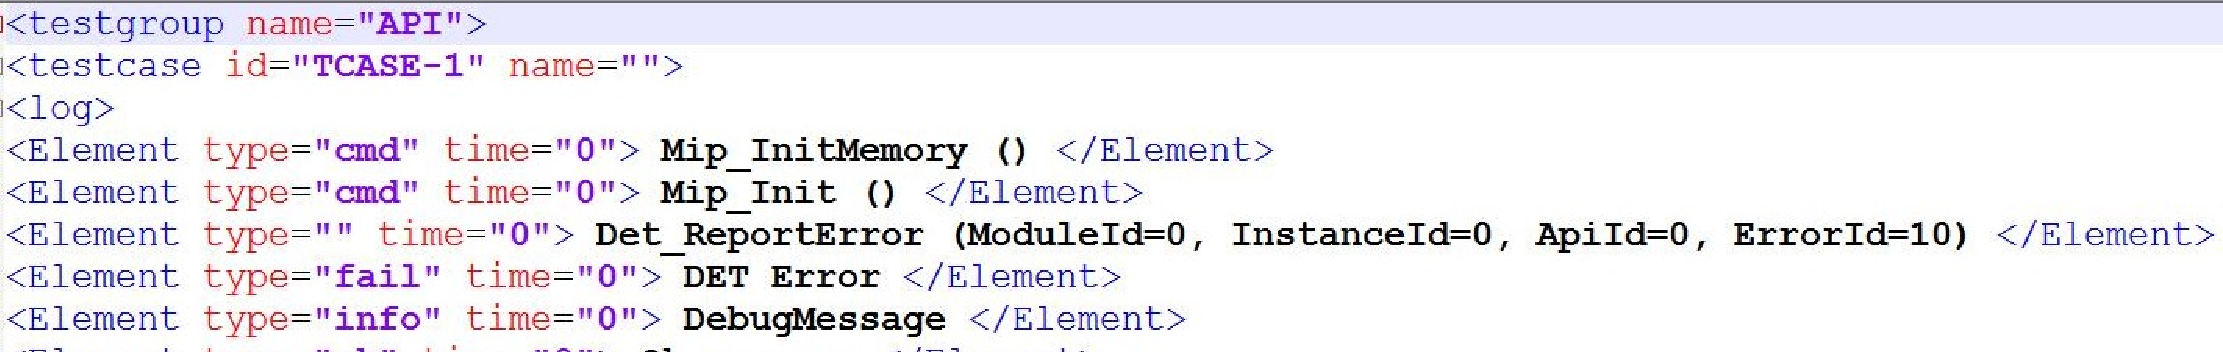
\includegraphics[scale=0.4]{./Bilder/ReportXML.pdf}
\caption{XML-Format eines VTR-Files, welches in Vector als Grundlage weiterer Testreviews verwendet wird.}
\label{fig:ReportXML}
\end{figure}
%

Bei der Verwendung des BTE-Tools auf einer beliebigen eingebetteten Hardware k�nnen bestimmte existierende Funktionalit�ten nicht wie gewohnt verwendet werden, damit beispielsweise die Testcases mit einer entsprechenden ID-Nummer gestartet und gekennzeichnet werden. Diese Initialisierung muss vor jeder Testcase-Durchf�hrung geschehen.

Die alte Methode \verb|BteTestCase_SetData( uint8 type, char *text )| soll durch eine verwandte Methode ersetzt werden, bei der lediglich die Testcase-ID-Nummer \texttt{testcaseID} bzw. kein String �bergeben wird. Der User ist deswegen angewiesen, stattdessen folgende Methode aufzurufen:
%
\begin{lstlisting}[style=C_colored_smallfont, caption = {Ausschnitt aus BteTestHandler.c}, label={lst:BteTestCase_SetData_ID}]
...
void BteTestCase_SetData_ID( uint16 id_num )
{
  bteTestSequence.id_num = id_num;
}
...
\end{lstlisting}
%
Weitere Anpassungen wurden im internen Funktionsbereich der BTE-Tools durchgef�hrt. Nur so sind die erw�hnten Anforderungen erf�llbar\footnote{Diese �nderungen sind f�r den Anwender nicht relevant und brauchen von ihm deswegen nicht weiter behandelt zu werden.}. 
%
\subsection*{Implementierung der Datenspeicherung}
%
Zur Implementierung der Speicherung des Testreports auf dem RAM werden zwei unterschiedliche Ans�tze ber�cksichtigt. Der der erste Ansatz weist bestimmte Nachteile auf, deshalb wird auf diese nur kurz eingegangen. Die zweite M�glichkeit wird dahingegen ausf�hrlicher behandelt, denn auf ihr basieren die L�sungsergebnisse der vorliegenden Aufgabe. 

Bei jedem der erw�hnten L�sungsans�tze ist eine geignete Kodierung der Daten in Form eines geigneten Protokolls notwendig, welches die Datenspeicherung auf dem RAM verwaltet.

\textbf{Report in Form einer Struktur (\texttt{stBteLogList}}):  

Der erste Ansatz, die Liste anhand einer Struktur abzuspeichern, wird durch \lstref{lst:structList} beschrieben. Dabei ist ersichtlich, dass der Datentyp \texttt{stBteLogList} aus einem 16-bit langen Eintrag (\textit{size}) und einer weiteren Struktur \verb|elem| vom Typ \texttt{stBteEventLog} besteht. Letztere enth�lt zwei weitere Datentypen (\textit{code} und \textit{data}). 
%
\begin{lstlisting}[style=C_colored_smallfont, caption = {Ausschnitt aus in Aufgabe 2 erstellten Sourcefile BteLogList.c}, label={lst:structList}]
typedef struct stBteEventLog 
{
  uint16 code;
  uint32 data;
} tBteEventLog;

typedef struct stBteLogList 
{
  uint16     size;
  tBteEventLog   elem[kBteLogList_size];
} tBteLogList;
\end{lstlisting}
%

Der Testreport wird auf Basis dieser beiden Strukturen im RAM des eingebetteten Prozessors abgelegt. Diese Struktur muss unterschiedliche Kennungen enthalten, welche zusammen das genannte Protokoll definieren. Damit ist eine hierachiche Trennung der gespeicherten Daten und deren Unterscheidung f�r eine geeignete Dekodierung gew�hrleistet. Tabelle \ref{tab:Protokoll1} zeigt eine beispielshafte Auswahl der verwendeten Kennungen.
%
\begin{table}[ht]
% title of Table
\centering 
% used for centering table
\begin{tabular}{c c c c}
% centered columns (4 columns)
\hline
\hline                        %inserts double horizontal lines
Kodierung & Beschreibung \\ [0.5ex]% inserts table 
%heading
\hline
0xFF & Kennung eines Testcases\\
\hline
0x21 & Kennung f�r 1. Datenelement\\
\hline
0x22 & Kennung f�r 2. Datenelement\\
\hline
0x23 & Kennung f�r 3. Datenelement\\
\hline
0x24 & Kennung f�r 4. Datenelement\\
\hline
0x25 & Kennung f�r 5. Datenelement\\ [1ex]      % [1ex] adds vertical space
\hline
%inserts single line
\end{tabular}
\caption{Verwendete Kennungen zur Unterscheidung der RAM-Bereiche, wo der Testreport gespeichert ist.}
\label{tab:Protokoll1}
% is used to refer this table in the text
\end{table}
%
\newpage
Wird ein neuer Testreport erstellt, dann wird am Anfang die L�nge \texttt{size} von \texttt{tBteLogList} auf Null gesetzt. Dadurch werden alle alten Eintr�ge der Liste �berschrieben bzw. gel�scht. Im n�chsten Schritt werden in Abh�ngigkeit der vorgegebenen Testcases die definierten Kennungen innerhalb der vorhandenen Elementen der Liste \texttt{elem} abgespeichert. 

Die einzelnen Elementen \texttt{elem} werden dabei in Abh�ngigkeit des Datentyps mithilfe von Bitverschiebungsoperationen so bef�llt, dass dabei folgenden Informationen vorkommen:
%
\begin{table}[ht]
% title of Table
\centering 
% used for centering table
\begin{tabular}{c c c c}
% centered columns (4 columns)
\hline
\hline                        %inserts double horizontal lines
Variablenname & Bezeichnung \\ [0.5ex]% inserts table 
%heading
\hline
\texttt{testcaseID} & Testcase-ID-Nummer\\
\hline
\texttt{numParam} & die Anzahl an �bergebenen Parameter\\
\hline
\texttt{type} & Event-Typ\\
\hline
\texttt{comp} & Component-ID-Nummer\\
\hline
\texttt{code} & Event-Code \texttt{code}\\
\hline
\texttt{time} & Zeitstempel\\
\hline
\texttt{data\_XYZ} & �bergebene Parametern\\ [1ex]      % [1ex] adds vertical space
\hline
%inserts single line
\end{tabular}
\caption{Relevanten Daten eines Events bei einem beliebigen Testcase.}
\label{tab:relevDatenEvents}
% is used to refer this table in the text
\end{table}
%

Abbildung \ref{fig:Protocol1} zeigt, wie das Protokoll bei dieser Art der Abspeicherung des Testreports auf dem RAM des eingebetteten Prozessors implementiert wird. 
%
\begin{figure}[!htp]
\centering
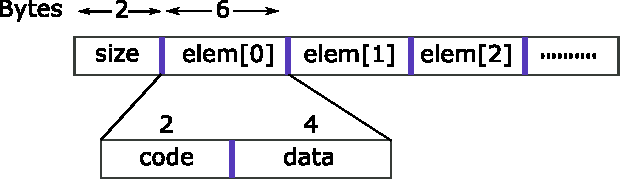
\includegraphics[scale=0.8]{./Bilder/Protocol12.pdf}
\caption{Struktur des RAM-Speichers bei Implementierung des Testreports in Form eines \texttt{struct}-Datentyps.}
\label{fig:Protocol1}
\end{figure}
%

Nachteilig dabei ist, dass der Compiler die gr��e des Bereichs so gro� wie der gr��te, in der Liste \texttt{tBteLogList} vorkommende Variablentyp festlegt. Jede Variable wird somit wie eine 32-Bit gro�e Variable behandelt (\verb|uint32|). Der Compiler wird deshalb f�r jede Variable immer einen 32-Bit gro�en Speicherplatz reservieren. Dies f�hrt zu Speicherplatz-Verschwendung, wenn es sich bei den abzuspeichernden Daten lediglich um 8-Bit gro�e Variablen handeln sollte. 

Dies l�sst sich dadurch vermeiden, dass spezielle Compiler-Einstellungen durchgef�hrt werden, was aber noch mehr Zeit in Anspruch nehmen w�rde.
\newpage
%
\section*{Zehnte Woche}
%
W�hrend dieser Woche galt meine Arbeit weiterhin der L�sung der 2. Aufgabe. Die zweite M�glichkeit der Kodierung und Abspeicherung des Reports wird hierbei eingef�hrt und beschrieben. 

\textbf{Report in Form eines Byte-Arrays \texttt{BteLogArray}}: 

Der Report wird in Form eines normalen Arrays \texttt{BteLogArray} vom Typ \verb|uint8| im RAM des betrachteten Prozessors abgespeichert. 
Die verarbeiteten Informationen bei den Methodensaufrufen werden ebenfalls sequenziell innerhalb des Arrays abgelegt. Dabei richtet sich die Abspeicherung der Daten nach den in folgender Tabelle festgelegten Kennungen.
%
\begin{table}[ht]
% title of Table
\centering 
% used for centering table
\begin{tabular}{c c}
% centered columns (4 columns)
\hline
\hline                        %inserts double horizontal lines
Kodierung & Beschreibung \\ [0.5ex]% inserts table 
%heading
\hline                  % inserts single horizontal line
0xFF & Kennung eines neuen Testcases \\
% inserting body of the table
0x5C & Kennung f�r End of file \\
0x6E & Kennung f�r End of file  \\ [1ex]      % [1ex] adds vertical space
\hline
%inserts single line
\end{tabular}
\label{tab:Protokoll2}
\caption{Verwendete Kennungen zur Unterscheidung der RAM-Bereiche, wo der Testreport gespeichert ist.}
% is used to refer this table in the text
\end{table}
%

Offensichtlich werden dabei nur der Anfang und das Ende des Report gekennzeichnet. Die Daten, die bei den einzelnen Methodensaufrufe ebenfalls im Report abzuspeichern sind, lassen sich allein durch die Kenntnis der Anzahl an �bergebenen Paratemern wieder rekonstruieren \footnote{Dies geschieht beim Dekodieren des Testreports anhand des PERL-Skripts, dessen Umsetzung noch beschrieben wird.}. Au�erdem wei� man dar�ber Bescheid, dass bei jedem neuen Testcase die in Tabelle \ref{tab:relevDatenEvents} angegebenen Variablen auf dem Report auszugeben sind.

Da in der Regel die �bergebenen Parameter und manche Daten, die auf dem Testreport vorkommen, nicht vom kleinsten Datentyp \texttt{uint8} sind sondern gr��er (\texttt{uint16} bzw. \texttt{uint32}), kann deren Inhalt nicht direkt in die einzelnen Eintr�ge des Byte-Arrays passen. Vor der Abspeicherung m�ssen diese Informationen deshalb so zerlegt und angepasst werden, dass sie immer in den 8-Bit gro�en Eintr�gen des genannten Arrays hinein passen. 

Diese Datenanpassung wird mithilfe der in \lstref{lst:ArrayList} gezeigten Methoden durchgef�hrt. Dabei werden die ben�tigten Daten nicht nur zerlegt, sondern auch direkt in dem Array gespeichert. 
\clearpage
\begin{lstlisting}[style=C_colored_smallfont, caption = {Ausschnitt aus BteLogList.c}, label={lst:ArrayList}]

void BteLogList_Serialize32(uint32 data)
{
  BteLogArray[kBteLogArray_position++] = (uint8)(data>>24);
  BteLogArray[kBteLogArray_position++] = (uint8)((data>>16) & 0xFF);
  BteLogArray[kBteLogArray_position++] = (uint8)((data>>8) & 0xFF);
  BteLogArray[kBteLogArray_position++] = (uint8)(data & 0xFF);
}

void BteLogList_Serialize16(uint16 data)
{
  BteLogArray[kBteLogArray_position++] = (uint8)((data>>8) & 0xFF);
  BteLogArray[kBteLogArray_position++] = (uint8)(data & 0xFF);
}
\end{lstlisting}

In Abbildung \ref{fig:Protocol2} wird ein Beispiel der Anordnung der gespeicherten Daten im RAM gezeigt. Variablen, die in kleineren 8-bit Datenfeldern zerlegt wurden, sind \verb|testcaseID|, \verb|time| und \verb|dataXYZ|. Der Inhalt der betrachteten Variable \verb|BteLogArray|, wo der Testreport sich befindet, wird dabei desto gr��er, je mehr Testf�lle, Methodensaufrufe und �bergebenen Parametern bei den zu testenden Funktionen vorkommen. 
%
\begin{figure}[!htp]
\centering
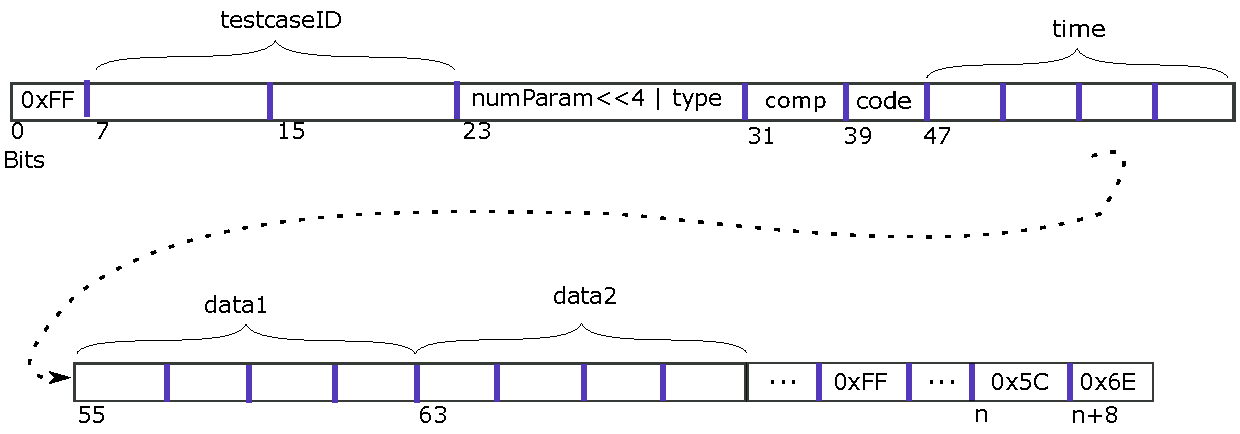
\includegraphics[scale=0.7]{./Bilder/Protocol2_cropped.pdf}
\caption{Struktur des RAM-Speichers bei Implementierung des Testreports in Form eines \texttt{uint8}-Array-Datentyps.}
\label{fig:Protocol2}
\end{figure}
%

Auf dieser Art und Weise wird mit den knappen, zur Verf�gung stehenden Hardwareressourcen m�glichst sparsam umgegangen. Jedes Feld des Arrays ist dadurch mit relevanten Daten vom Testreport bef�llt, was dazu f�hrt, dass m�glichst wenig Speicherplatz verschwendet wird.

Nach einer erfolgreichen Speicherung der Daten in den RAM des eingebetteten Systems, sieht der Speicherbereich wie im Bild \ref{fig:EclipseHardwareMem} aus. Mithilfe des GDB-Debuggers ist es dann m�glich, den relevanten Speicherbereich direkt als Bin�rdatei auf den lokalen PC zu exportieren. Dazu ist es deswegen notwendig, dass ein Hardware-Debugger zur Versf�gung steht. Auf Basis dieser Datei und einer \verb|PERL|-Anwendung wird die Rekonstruktion des entsprechenden Reports angesetzt. Dieser Ansatz wird im n�chsten Kapitel n�her erkl�rt.
%
\begin{figure}[!htp]
\centering
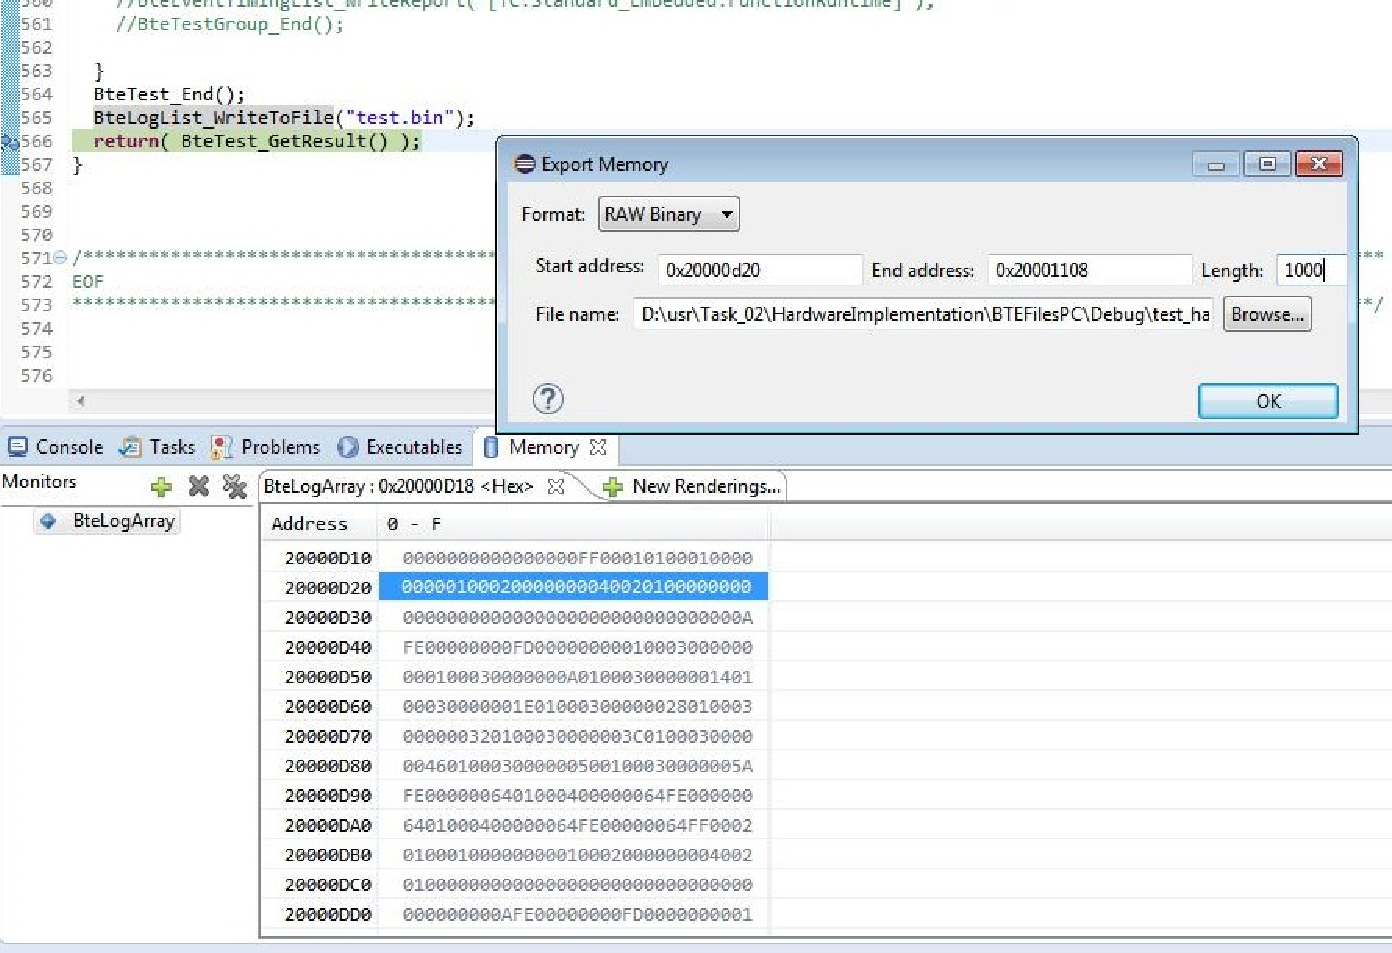
\includegraphics[scale=0.7]{./Bilder/EclipseHardwareMem.pdf}
\caption{Eclipse-Funkitonalit�t zur Verwendung vom GDB-Debugger. Dabei l�sst sich ein bestimmter Speicherbereich vom eingebetteten Prozessor entnehmen und als Bin�rdatei auf dem lokalen Rechner abspeichern.}
\label{fig:EclipseHardwareMem}
\end{figure}
%
\clearpage
%
\section*{Elfte Woche}
%
\subsubsection*{Dekodierung und Rekonstruktion eines XML-Testreports}
%
Ein Ansatz, um aus der Bin�rdatei ein Report zu erstellen, ist, diese Datei mithilfe einer in einer Skriptsprache programmierten Anwendung zu analysieren und verarbeiten. Entsprechende Algorithmen k�mmern sich um die Dekodierung und Ausgabe der Daten als ein XML-File. Der auf dieser Art und Weise erstellte Report soll letztendlich bis auf kleine Details im Text genauso aussehen, wie ein Testreport, welcher mithilfe des BTE-Frameworks auf dem PC erstellt w�rde. 

Die Main-Methode \verb|ConvertBin2Vtr| des erstellten \verb|PERL|-Skripts wird in \lstref{lst:PERL_XMLRepMain} gezeigt. Die Struktur dieser Methode zeigt explizit die Struktur der gesammten programmierten Anwendung. 
%

\begin{lstlisting}[style=PERL_st, caption = {PERL-Skript zum Einlesen bzw. zur Verarbeiten einer Bin�rdatei.\\ Anschlie�end wird ein Testreport aus den gewonnenen Daten erstellt.},label={lst:PERL_XMLRepMain}]
# Main function
sub ConvertBin2Vtr
{
  # read the binary file containing the data of the data of the test report
  my $binFile_path = $ARGV[0];
	# read the path where the report file has to be stored
  my $vtrFile_path = $ARGV[1];
  
  # read the transformation rules from the configuration file
  LoadEventConfig($ARGV[2]);

  # get the relevant data
  GetBinaryContent($binFile_path);

  # process the binary data and write to vtr
  OpenVtr($vtrFile_path);
  ProcessBinaryData();
  CloseVtr();
}
\end{lstlisting}
%

In Zeile 5 wird die Bin�rdatei �ber das Kommando \texttt{\$ARGV[0]} eingelesen. Dieser Aufruf bezieht sich auf das 1. Argument, welcher dem programmierten \verb|PERL|-Skript �bergeben wird. Dies kann �ber die Ausf�hrung eines sogenannten Batch-Skripts ausgef�hrt werden. Die Batch-Funktionalit�ten �hneln den Funktionalit�ten der Windows-Kommandozeile. Wie der programmierte \verb|PERL|-Skript ausgef�hrt und die Bin�rdatei geladen werden k�nnen, wird bespielhaft anhand eines Batch-Skript in \lstref{lst:Batch} gezeigt.
%
\newpage
%
\begin{lstlisting}[style=Batch_st,caption = {Batch-Aufruf vom erstellten \texttt{PERL}-Skript. Dabei ist ersichtlich wie nicht nur der \texttt{PERL}-Skript ausgef�hrt wird, sondern auch weitere Files wie die Bin�rdatei, ein Userfile und das anschlie�end auszugebende Reportfile.},label={lst:Batch}]
@echo off
rem the following command can be used if the files in the parameter lies in the same path like the perl file
perl bin2xml_v2.pl test.bin AnwenderFile1.txt BteReport_Log.xml
pause
\end{lstlisting}
%
Desweiteren muss nach dem Einladen der Bin�rdatei eine entsprechende Vorvearbeitung derselbe stattfinden. Dies wird in Zeile 13 vom \lstref{lst:PERL_XMLRepMain} durchgef�hrt und ist deswegen notwendig, weil die relevanten Daten des Testreports nicht im gesammten \texttt{BteLogArray} enthalten sind, diese nur ein Teil davon belegen. Die restlichen Daten sind deshalb zu entfernen.

Die in Zeile 17 gezeigte Methode \texttt{ProcessBinaryData()} beinhaltet die eigentliche Dekodierung der Daten und Erstellung des Testreports. Im Anschluss der Dekodierung der Daten wird die Testreport-Datei auf die Festplatte gesichert.

Die oben genannten Schritten, die in der Main-Methode der \verb|PERL|-Anwendung durchgef�hrt werden, sind in Form einer State-Maschine in Abbildung \ref{fig:StateMaschPERL} dargestellt. In dem Zustand \textit{AnalyseReadByte} �berpr�ft der Suchalgorithmus die Natur des eingelesenen Bytes. In Anbh�ngigkeit derselben gibt es Transitionen in den benachbarten Zust�nden, wo die Daten dekodiert werden und der Testreport gleichzeitig aktualisiert wird.

Ein Ausschnitt vom erstellten \verb|PERL|-Skript kann in \lstref{lst:PERL_XML_Binary} gefunden werden. Das oben gezeigte Diagramm erg�nzt die Software-Spezifikation dienen.
%\begin{landscape}
\begin{figure}[!htp]
\centering
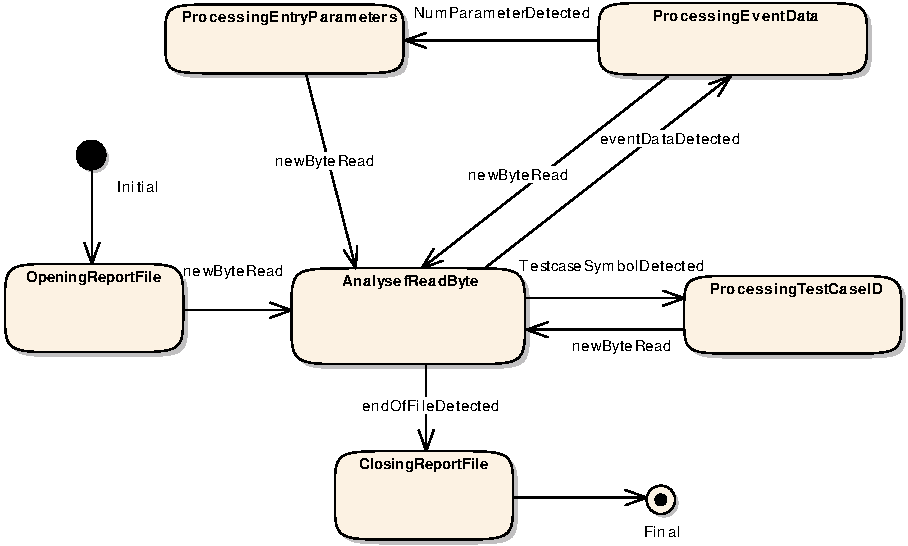
\includegraphics[scale=0.9]{./Bilder/StateMaschPERL_cropped.pdf}
\caption{State-Chart-Diagramm, welches die Funktionsweise der erstellte PERL-Anwendung n�her beschreibt.}
\label{fig:StateMaschPERL}
\end{figure}
%\end{landscape}
%
\newpage
%
\section*{Zw�lfte Woche}
%
In der vorliegenden Woche war meine Aufgabe das \verb|PERL|-Programm zu dokumentieren und besser zu strukturieren. Nur so ist es m�glich, in der Zukunft das erstellte bzw. modifizierte Tool zu pflegen und warten. 
%
\subsubsection*{Gesamte Struktur des erweiterten Anwendungfalls}
%
Der in \figvref{fig:BTEUseCase} gezeigte Anwendungsfall \textit{execute test on embedded device} konnte durch die Anpassungen der vorhandenen Struktur des BTE-Tools und die Erstellung eines \verb|PERL|-Skripts realisiert werden. Seine gesammte Funktionalit�t wird in Abbildung \ref{fig:BTELogListStruktur} in Form eines Klassendiagramms dargestellt.

Die gelb markierten Klassen stellen die bereits vorhandenen Funktionalit�ten dar, die gegebenenfalls modifiziert werden mussten. Diese sind ebenfalls in \figvref{fig:BTELogListold} dargestellt.

Die wei�en Klassen erweitern den Funktionsumfang und wurden zur L�sung der vorliegenden Aufgabe. Diese erm�glichen die Lauff�higkeit des BTE-Tools auf einem beliebigen eingegebetteten System und die Erstellung eines entsprechenden Testreports.

Dabei ist zu erkennen, dass das gesammte BTE-Tool auf dem eingebetteten Echtzeitsystem l�uft und dabei �ber das erstellte \verb|LogList|-Modul die relevanten Informationen vom Testreport auf den LogList-Array speichert. Das Debugger-Modul k�mmert sich um das Extrahieren der Bin�rdatei vom RAM des betrachteten Systems, wobei es anzumerken ist, dass dies manuell erfolgen muss. 

Auf der PC-Seite befindet sich neben der extrahierten Bin�rdatei die programmierten \verb|PERL|-Anwendung, welche sich zus�tzlich eines vom User vorgegebenen Konfigurationsfiles bedient, um den gew�nschten Testreport zu erstellen.
%
%\begin{landscape}
\begin{figure}[!htp]
\centering
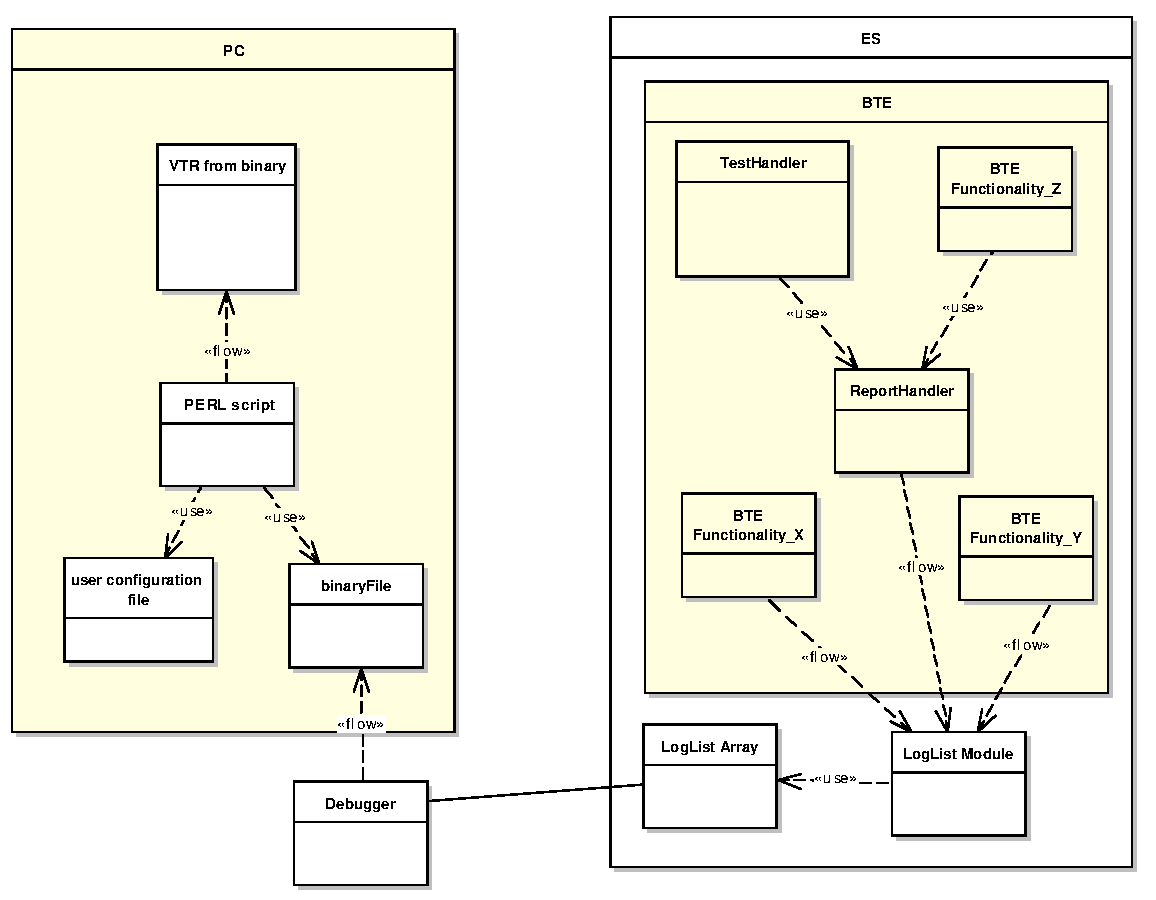
\includegraphics[scale=0.8]{./Bilder/BTELogList_cropped.pdf}
\caption{Klassendiagramm zur Erg�nzung der Softwarespezifikation des erweiterten BTE-Tools. Dabei k�nnen die funktionalen Zusammenh�nge zwischen den alten und neuen Modulen erkannt werden.}
\label{fig:BTELogListStruktur}
\end{figure}
%\end{landscape}
%
\section{Validierung und Ergebnisse der 2. Aufgabenstellung}
%
Um die G�ltigkeit der programmierten Anwendungen zu �berpr�fen, werden zwei Testreports einer beliebigen Software-Komponente erstellt.

Die Tests werden jeweils auf dem PC und der in \figvref{fig:discovery} gezeigten Hardware durchgef�hrt. Am Ende jeden Tests entstehen zwei unabh�ngige Bin�rdateien, die die Testreports enthalten. Auf dem PC werden die zwei Dateien mithilfe der \verb|PERL|-Anwendung analysiert und in ein entsprechendes XML-File konvertiert. Beide Dateien werden in Abbildung \ref{fig:reports} miteinander vergliechen. Dabei stellt man fest, dass beide Reports die gleiche Eigenschaften aufweisen, was auf die Korrektheit der implementierten Anwendung schlie�en l�sst.
%
\begin{landscape}
\begin{figure}[!htp]
\centering
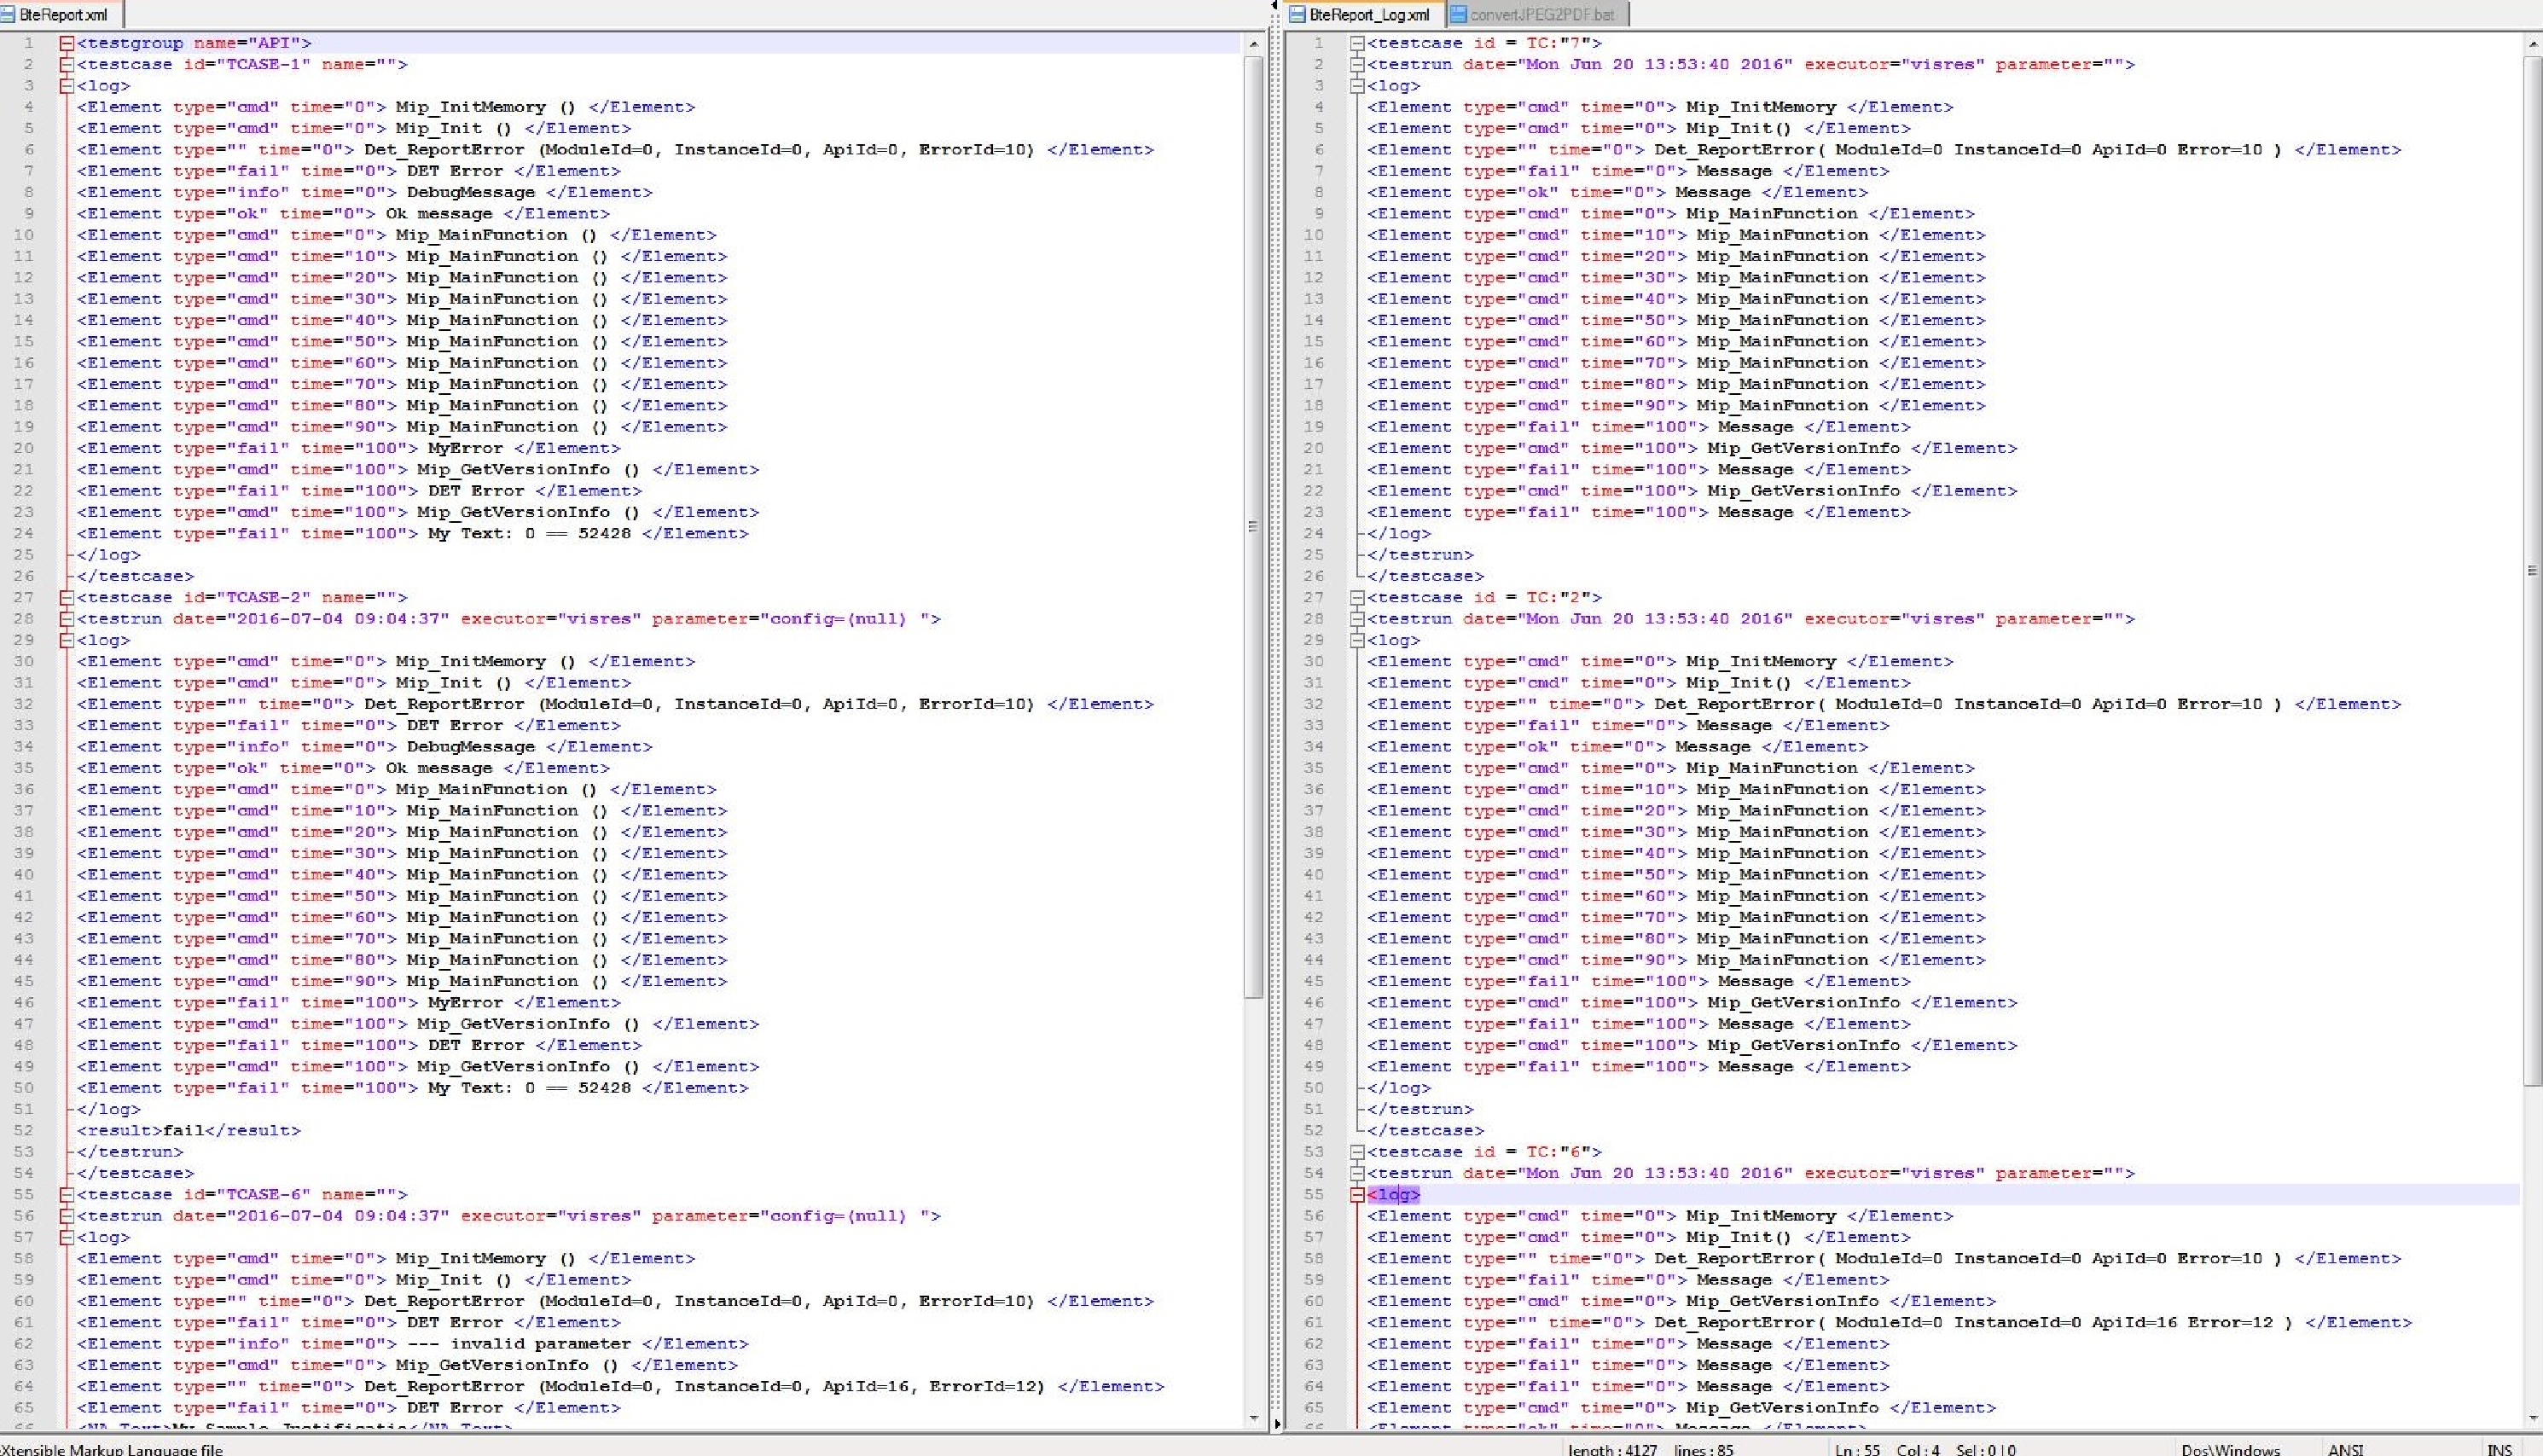
\includegraphics[width=200mm,height=150mm]{./Bilder/reports.pdf}
\caption{Testreports, die aus zwei unterschiedlichen Bin�rdateien erstellt worden sind. Die eine Bin�rdatei wird nach Testdurchf�hrung auf PC und die zweite auf dem eingebetteten Prozessor erstellt.}
\label{fig:reports}
\end{figure}
\end{landscape}
%
%
\chapter{Zusammenfassung und Ausblick}
%
Im Rahmen des Praktikums bei Vector bekam ich die Gelegenheit, in der PES Abteilung mitzuarbeiten. Dabei sammelte ich wertvolle Einblicke und Erfahrungen sowohl in die Firmenabteilungen und als auch in einzelne Projekte. 

Das Ziel meiner Arbeit bestand vorwiegend darin, den Umgang mit unterschiedlichen Softwaretools zu erlernen, die w�hrend der Entwicklung von verschiedenen Software-Produkten in der Abteilung eingesetzt werden.

Gleichzeitig war es mir m�glich, w�hrend meines Aufenthalts wertvolle Kontakte zu kn�pfen und Gespr�che zu f�hren, die f�r mein weiteres ber�fliches und pers�nliches Leben ein gro�er Gewinn sind.






% =================================================================================
% Anhang
% =================================================================================
\appendix % Damit wird der Anhang begonnen. Die Kapitel werden ab jetzt mit Buchstaben nummeriert

\chapter{ Auschnitt der Softwaredokumentation}\label{cha:tools}
%
Im Rahmen dieser Arbeit sind folgende Software-Tools entwickelt worden:
\begin{itemize}
\item \textbf{Schwerpunktlage der Verbrennung} \\
\verb+SPL = function_SPL(phi_mod,QB,abtastzeit_s,nMot)+ berechnet.
\item \textbf{Zylinderdruckgradient} \\
 \verb+[dp_dphi,ddp_ddphi]  = Grad_dGrad_pZMax(phi,pZ)+
\end{itemize}
%
Die oben genannten Tools werden im Folgenden n�her erl�utert.
%
\section{Datei�bertragung }
%

\begin{lstlisting}[style=PERL_st, caption = {PERL Datei�bertragung},label={lst:PERL_Dateiueb}]

#!/Dwimperl/perl/bin/perl.exe -w
use strict;
use File::Copy;
use Cwd;

my $workingdir =cwd();	# find the directory where the script is being run
my $target_loc = "$workingdir/Relevant";	# set the target directory for the files
mkdir $target_loc;

# file where the paths of the source and header files are indicated 
open (PRJ_QAC , "$workingdir/Folder.prj")
or die "Fehler beim Oeffnen von '$workingdir/Baseline/Folder.prj': $!\n";

my @zeilen = <PRJ_QAC>;
my @var_arr;
my $var_str;
# hilfsvariablen
my $h1 = 0;	# wird der Anfangpunkt der Source-Pfade
my $h2 = 0;	
my $h3 = 0;	# wird der Endpunkt der Source-Pfade

# es muss ermoeglicht werden, den Punkt zu finden, ab dem die Source-Pfade ausgelesen werden koennen

foreach(@zeilen){	# iteriere ueber die Einstellungsdatei
	
	my $hola = 4;
	
	if($_ =~ /CompPers/){	# suche nach dem patern
		$h3 = $h1;	# wurde der Patern gefunden, dann halte die Zeilenummer -h1- fest und fange eine neue Suche ab dem Ort an
		for (my $p = $h1+1 ;$p < @zeilen ; $p++){
			if($zeilen[$p] =~ /EndContainedFilesMarker/){
				last;	# verlasse innere for-Schleife
			}
		$h3++
		}
		last;	# verlasse aeussere for-Schleife
	}	
	$h1++;
}

for(my $t = $h1+1;$t <= $h3; $t ++ )	{ #wird ueber Datei iteriert
	
	
	@var_arr = split(/\\/,$zeilen[$t]);	# trenne Zeile in Array ueber \ Zeichen
	$var_str = $var_arr[$#var_arr];		# bekomme letzter Eintrag des Arrays
	
	
	$h2 = $zeilen[$t];
	$h2 =~ tr/\\/\//;
		
	$target_loc = $target_loc."/$var_str";
	
	chomp($target_loc);
	chomp($h2);

	print "$target_loc\n";	# gebe aus, welche Dateien kopiert werden


	copy($h2, $target_loc) or die "File cannot be copied.";
	
	$target_loc = "$workingdir/Relevant";
	
}
\end{lstlisting}
%
\newpage
\section{Bearbeitung einer XML-Datei}
%
F�r die Echtzeitbestimmung der Kenngr��en Druckgradientenverlauf $\frac{dp}{d\phi}$ und deren zeitlichen Ableitung $\frac{d^2p}{d\phi^2}$ sind die momentanen Werte des simulierten Zylinderdrucks $p_Z$ und des Kurbelwinkels $\phi$ n�tig. Diese Kenngr��en werden vom Verbrennungsmodell ermittelt und k�nnen dementsprechend verarbeitet werden. In Abbildung \ref{fig:DruckgradSimulink} ist die entsprechende Embendded MATLAB Function zu erkennen. Der jeweilige Quellcode wird im Listing \ref{lst:Druckgrad} aufgezeigt.
%

\begin{lstlisting}[style=PERL_st, caption = {PERL XML},label={lst:PERL_XML}]
#!/Dwimperl/perl/bin/perl.exe -w
use strict;
use Cwd;

my $working = cwd();
my $string1 = "  \<file target=\"C\" name\=\"";
my $string2 = "\" folder\=\"=$working/Relevant\"\/\>";

my $z1 = 0;

# file where the paths of the source and header files are indicated 
open(LESEN1,"$working/Baseline/Folder.prj")
or die "Fehler beim Oeffnen von 'Folder.prj': $!\n";
# default file where the default information of the qac9 project is indicated
open(LESEN2,"prqaproject.xml")
or die "Fehler beim Oeffnen von 'prqaproject.xml': $!\n";

my @zeilen_files = <LESEN1>;
my @zeilen_xml = <LESEN2>;

close(LESEN1);
close(LESEN2);
unlink "prqaproject.xml";	# delete default file, afterwards a new file will be again created


my @var_arr;		#store the splited strings
my @var_arr_files;	#store the strings of the source files
my $var_str;
my $hilfsvar = 0;
my $h1 = 0;	# wird der Anfangpunkt der Source-Pfade
my $h2 = 0;	
my $h3 = 0;	# wird der Endpunkt der Source-Pfade
my $h1_xml = 0;
my $h2_xml = 0;


# es muss ermoeglicht werden, den Punkt zu finden, ab dem die Source-Pfade ausgelesen werden koennen
foreach(@zeilen_files){	# iteriere ueber die Einstellungsdatei
	
	if($_ =~ /CompPers/){	# suche nach dem Muster
		$h3 = $h1;	# wurde der Muster gefunden, dann halte die Zeilenummer -h1- fest und fange eine neue Suche ab dem Ort an
		for (my $p = $h1+1 ;$p < @zeilen_files ; $p++){
			if($zeilen_files[$p] =~ /EndContainedFilesMarker/){
				last;	# verlasse innere for-Schleife
			}
		$h3++
		}
		last;	# verlasse aeussere for-Schleife
	}	
	$h1++;
}


for(my $t = $h1+1;$t <= $h3; $t ++ )	{ #wird ueber Datei iteriert
	
	@var_arr = split(/\\/,$zeilen_files[$t]);	# trenne Zeile in Array ueber \ Zeichen
	# print $zeilen_files[$t]."\n";
	$var_str = $var_arr[$#var_arr];		# bekomme letzter Eintrag des Arrays, also den Namen der c-Datei
	
	$var_arr_files[$t-$h1-1] = $var_str;	# speichere die Namen der Datein in den entsprechenden Eintrag	
	
}	


foreach(@zeilen_xml){	# iteriere ueber die Einstellungsdatei
	
	if($_ =~ /\<\!-- Explicit files... --\>/){	# suche nach dem Muster
		$h2_xml = $h1_xml;	# wurde der Muster gefunden, dann halte die Zeilenummer -h1- fest und fange eine neue Suche ab dem Ort an
		for (my $p = $h1_xml+1 ;$p < @zeilen_xml ; $p++){
			if($zeilen_xml[$p] =~ /\<\/prqaproject\>/){
				last;	# verlasse innere for-Schleife
			}
		$h2_xml++
		}
		last;	# verlasse aeussere for-Schleife
	}	
	$h1_xml++;
}	

print $h1_xml."\n";
print $h2_xml."\n";
	
open(SCHREIBEN,"> prqaproject.xml")
or die "Fehler beim Oeffnen von 'prqaproject.xml': $!\n";


foreach(@zeilen_xml){
	
	if($z1 < $h1_xml+1){	# schreibe die Anfangszeilen zu der Datei
		print SCHREIBEN $zeilen_xml[$z1];
	} else {
		foreach(@var_arr_files){	# schreibe die Namen der Files in die Zieldatei
			chomp($_);
			print SCHREIBEN "$string1".$_."$string2\n";
		}
		print SCHREIBEN " \<\/files\>\n\<\/prqaproject\>";		
		last;
	}
	$z1++;	
}

close(SCHREIBEN) or die "Fehler beim Schliessen von 'prqaproject.xml': $! \n";
\end{lstlisting}
%
\newpage
\section{Erstellung eines XML-Testreports aus Bin�rdatei}
%
\begin{lstlisting}[style=PERL_st, caption = {Auschnitt vom File BteBin2Vtr.pl},label={lst:PERL_XML_Binary}]
#!/perl/bin/perl.exe -w

use strict;
use warnings;
use Time::Piece;

my @binFile_content;
my $binFile_length = 0;
my $binFile_index = 0;
my %event_map;
my $testcaseIsOpen = 0;

ConvertBin2Vtr();

#--------------------------------------------------------------
# Main function
sub ConvertBin2Vtr
{
  my $binFile_path = $ARGV[0];
  my $vtrFile_path = $ARGV[1];
  
  # read the transformation rules from the configuration file
  LoadEventConfig($ARGV[2]);

  # get the relevant data
  GetBinaryContent($binFile_path);

  # process the binary data and write to vtr
  OpenVtr($vtrFile_path);
  ProcessBinaryData();
  CloseVtr();
}

#--------------------------------------------------------------
# read the config file and store its content in event map
sub LoadEventConfig($)
{
  my $configFile_path = $_[0];
  
  # open config file
  open(configFile,$configFile_path) or die "Error while opening config file\n";  
  my @configFile_content = <configFile>;
  close(configFile);

  # store content of each line in event map
  # line layout: id(4 chars) text(x chars)
  # Example: 0105 This is my text
  foreach my $cfgFile_line (@configFile_content)
  {
    chomp($cfgFile_line);
    if (length($cfgFile_line) > 4)
    {
      my $event_id = substr($cfgFile_line,0,4);
      my $event_text = "";
      $event_text = substr($cfgFile_line,5);
      $event_map{$event_id} = $event_text; 
    }
  }
}

#--------------------------------------------------------------
sub GetBinaryContent($)
{
  my $binFile_path = $_[0];

  # open binary file for reading
  $binFile_length = -s "$binFile_path";
  open(binFile,"$binFile_path") or die "Error: opening binary file: $binFile_path\n";
  binmode(binFile);

  # read content
  my $binFile_string;
  read(binFile, $binFile_string, $binFile_length);
  close(binFile);
  
  # short the content (until EOF marker)
  @binFile_content = split("", $binFile_string);
  $binFile_length = GetIndexOfEOF($binFile_string);
  if ($binFile_length == -1) 
  {
    print "Warning: EOF-symbol not found\n";
  }
  else
  {
    @binFile_content = @binFile_content[0..$binFile_length];
  }
}

#--------------------------------------------------------------
sub ProcessBinaryData($)
{
  # iterate over binary data
  # data layout: kind(1 byte) data(x byte)
  do
  {
    my $data_kind = (BinFile_Read(1))[0];

    # detect what kind of data is present. Process data accordingly.
    if( $data_kind eq chr(hex 'FF'))
    {
      # TCASE
      # layout: kind (1 byte) id(2 byte)
      Process_TCASE(BinFile_Read(2));
    }
    elsif($data_kind eq chr(hex('FD')) || $data_kind eq chr(hex('FE')))
    {
      # message
      # type is coded in "kind"
      # layout: kind(1 byte) time(4 byte)
      my $message_kind=GetMessageType($data_kind);
      Process_Message($message_kind, BinFile_Read(4));
    }
    else
    {
      # event
      # type and size are coded in "kind"
      # layout: kind(1 byte) id(2 byte) time(4 byte) data(4*dlc byte)
      my $event_type = GetEventType($data_kind);
      my $event_size = GetEventSize($data_kind);
      my @event_data = BinFile_Read(6 + 4*$event_size);
      Process_Event($event_type, @event_data);
    }
  } while($binFile_index < $binFile_length);
}
...
\end{lstlisting}

%\chapter{Befehle in commonmacros.tex}
\label{cha:commonmacros}
Hier sind im Folgenden kurz die in \texttt{commonmacros.tex} definierten Befehle aufgelistet.
%
\section*{Einheiten}
Die folgenden Befehle funktionieren im Mathe-und Textmodus (\dah es wird im Textmodus automatisch f�r den Befehl in den Mathemodus umgeschaltet):
\begin{itemize}
	\item Einheit (Aufrechte Schrift im Mathemodus)\\ \verb|\unit{\frac{N}{m}}| $\rightarrow$ \unit{\frac{N}{m}}
	\item Zahl mit Einheit\\(Setzt "`kleines"' Leerzeichen zwischen Zahl und Einheit, Zahl und Einheit automatisch im Mathemodus, Einheit in aufrechter Schrift)\\ \verb|\valunit{34,3}{cm}| $\rightarrow$ \valunit{34,3}{cm}
	\item (Das aufrechte $\mu$ gibt es mit dem Befehl \verb|\upmu| aus dem Paket upgreek)\\ \verb|\valunit{4}{\upmu m}| $\rightarrow$ \valunit{4}{\upmu m}
\end{itemize}

\noindent Besondere Einheiten
\begin{itemize}
	\item Gradzeichen (Funktioniert im Text- und Mathemodus)\\ \verb|\degree| $\rightarrow$ \degree
	\item Grad Celsius (Funktioniert im Text- und Mathemodus)\\ \verb|\degC| $\rightarrow$ \degC
\end{itemize}


\section*{Vektoren und Matrizen}
\begin{itemize}
	\item Vektor\\ \verb|\ve{x}| $\rightarrow$ \ve{x}
	\item Matrix\\ \verb|\ma{A}| $\rightarrow$ \ma{A}
	\item Vektor Sonderzeichen\\ \verb|\ves{\lambda}| $\rightarrow$ \ves{\lambda}
	\item Matrix Sonderzeichen\\ \verb|\mas{\Lambda}| $\rightarrow$ \mas{\Lambda}
\end{itemize}
Wichtig: Mathematische Akkzente m�ssen dabei geklammert werden!
\begin{itemize}
	\item \verb|$\dot{\ve{x}}$| $\rightarrow$  $\dot{\ve{x}}$
	\item \verb|$\dot{\tilde{\ve{x}}}$| $\rightarrow$ $\dot{\tilde{\ve{x}}}$
\end{itemize}
\verb|\ve{}| und \verb|\ma{}| \bzw \verb|\ves{}| und \verb|\mas{}| machen jeweils genau das gleiche. Die Unterscheidung dient nur zur besseren Lesbarkeit.

\begin{itemize}
	\item Transponiert-Zeichen (aufrechtes T)\\ \verb|$\ma{A}^\transp$| $\rightarrow$ $\ma{A}^\transp$
\end{itemize}


\section*{Funktionen und Abk�rzungen}

\begin{itemize}
	\item Unterstreichen\\ \verb|$\ul{x}$| $\rightarrow$ $\ul{x}$
	\item Innenprodukt\\ \verb|$\inprod{f}{g}$| $\rightarrow$ $\inprod{f}{g}$
	\item Exponentialschreibweise\\ \verb|$45\E{-2}$| $\rightarrow$ $45\E{-2}$
	\item e-Funktion\\ \verb|$\eexp{t}$| $\rightarrow$ $\eexp{t}$
	\item Rang\\ \verb|$\rang{\ma{A}}$| $\rightarrow$ $\rang{\ma{A}}$
	\item Imagin�re Einheit (aufrechtes j)\\ \verb|$5+\iu 2$| $\rightarrow$ $5+\iu 2$
	\item "`Von-Bis-Punkte"' mit Kommas und sch�nen Abst�nden\\ \verb|$1 \todots n$| $\rightarrow$ $1 \todots n$
	\item i abgeleitet\\ \verb|$\doti$| $\rightarrow$ $\doti$
	\item Aufrechte Schrift (Abk�rzung f�r \verb|\mathrm{}|) \\ \verb|$\mrm{abc}$| $\rightarrow$ $\mrm{abc}$
	\item Normaler Text in Formel (Abk�rzung f�r \verb|\textnormal{}|)\\ \verb|$\tn{ab f�r}$| $\rightarrow$ $\tn{ab f�r}$
	\item Geklammerte Gruppe mit Subscript\\ \verb|$\grpsb{\frac{1}{2}}{x}$| $\rightarrow$ $\grpsb{\frac{1}{2}}{x}$
	\item Geklammerte Gruppe mit aufrechtem Subscript\\ \verb|$\grprsb{\frac{1}{2}}{x}$| $\rightarrow$ $\grprsb{\frac{1}{2}}{x}$
	%\item \\ \verb|| $\rightarrow$
%	\item \\ \verb|| $\rightarrow$
\end{itemize}



\section*{Ableitungen und Integrale}

\begin{itemize}
	\item Normale Ableitung\\ \verb|$\normd{f}{x}$| $\rightarrow$ $\normd{f}{x}$
	\item Materielle Ableitung\\ \verb|$\matd{f}{x}$| $\rightarrow$ $\matd{f}{x}$
	\item Partielle Ableitung\\ \verb|$\partiald{f}{x}$| $\rightarrow$ $\partiald{f}{x}$
	\item Beispiel h�here Ableitung\\ \verb|$\normd{^2 f}{x^2} \qquad \partiald{^2 f}{x \partial y}$| $\rightarrow$ $\normd{^2 f}{x^2} \qquad \partiald{^2 f}{x \partial y}$
	\item Normale Ableitung an\\ \verb|$\normdat{f}{x}{x=0}$| $\rightarrow$ $\normdat{f}{x}{x=0}$
	\item Materielle Ableitung an\\ \verb|$\matdat{f}{x}{x=0}$| $\rightarrow$ $\matdat{f}{x}{x=0}$
	\item Partielle Ableitung an\\ \verb|$\partialdat{f}{x}{x=0}$| $\rightarrow$ $\partialdat{f}{x}{x=0}$
	\item Aufrechtes "`d"' f�r Integral\\ \verb|$\ud$| $\rightarrow$ $\ud$
	\item Beispiel f�r Integral\\ \verb|$\int f(x) \ud x$| $\rightarrow$ $\int f(x) \ud x$
\end{itemize}


\section*{Transformationen}

\begin{itemize}
	\item \verb|$\Laplace{x}$| $\rightarrow$ $\Laplace{x}$
	\item \verb|$\InvLaplace{X}$| $\rightarrow$ $\InvLaplace{X}$
	\item \verb|$x \trans X$| $\rightarrow$ $x \trans X$
	\item \verb|$X \invtrans x$| $\rightarrow$ $X \invtrans x$
	\item \verb|$\FT{x}$| $\rightarrow$ $\FT{x}$
	\item \verb|$\FTabs{x}$| $\rightarrow$ $\FTabs{x}$
	\item \verb|$\IFT{x}$| $\rightarrow$ $\IFT{x}$
	\item \verb|$\DFT{x}$| $\rightarrow$ $\DFT{x}$
	\item \verb|$\DFTabs{x}$| $\rightarrow$ $\DFTabs{x}$
\end{itemize}



\section*{Matlab/Simulink}

\begin{itemize}
	\item \verb|\mlfct{abc}| $\rightarrow$ \mlfct{abc}
	\item \verb|\mlvar{abc}| $\rightarrow$ \mlvar{abc}
\end{itemize}



\section*{Verweise}

Verweise auf verschiedene Objekte mit passendem Text ("`Abbildung X"', "`Tabelle X"'). Dabei ist dann immer der komplette Text ein Hyperlink, und nicht nur die Zahl.
\begin{itemize}
	\item Abbildung\\ \verb|\figref{label}|
	\item Tabelle\\ \verb|\tabref{label}|
	\item Gleichung\\ \verb|\equref{label}|
	\item Definition\\ \verb|\defref{label}|
	\item Kapitel\\ \verb|\charef{label}|
	\item Abschnitt\\ \verb|\secref{label}|
	\item Listing\\ \verb|\lstref{label}|
	\item Seite\\ \verb|\pagerefh{label}|
\end{itemize}

\ZT auch auf Varioref basierend ("`Abbildung 23 auf dieser Seite"', "`Abbildung 23 auf Seite 45"')
\begin{itemize}
	\item Abbildung\\ \verb|\figvref{label}|
	\item Tabelle\\ \verb|\tabvref{label}|
	\item Gleichung\\ \verb|\equvref{label}|
\end{itemize}


\section*{Abk�rzungen}
Abk�rzungen mit Punkt "`dazwischen"' (wird mit kleinen Abst�nden gesetzt)\\
\verb|\dah| $\rightarrow$ \dah, \verb|\Dah| $\rightarrow$ \Dah, \verb|\iA| $\rightarrow$ \iA, \verb|\IA| $\rightarrow$ \IA, \verb|\ua| $\rightarrow$ \ua, \verb|\Ua| $\rightarrow$ \Ua, \verb|\uU| $\rightarrow$ \uU, \verb|\UU| $\rightarrow$ \UU, \verb|\zB| $\rightarrow$ \zB, \verb|\ZB| $\rightarrow$ \ZB, \verb|\zT| $\rightarrow$ \zT, \verb|\ZT| $\rightarrow$ \ZT

\vspace{1ex}
\noindent Abk�rzungen mit Punkt, bei denen der Punkt nicht als Satzende interpretiert wird:\\
\verb|\bspw| $\rightarrow$ \bspw, \verb|\Bspw| $\rightarrow$ \Bspw, \verb|\bzw| $\rightarrow$ \bzw, \verb|\Bzw| $\rightarrow$ \Bzw,  \verb|\bzgl| $\rightarrow$ \bzgl, \verb|\ca| $\rightarrow$ \ca, \verb|\evtl| $\rightarrow$ \evtl, \verb|\ggf| $\rightarrow$ \ggf, \verb|\Ggf| $\rightarrow$ \Ggf, \verb|\usw| $\rightarrow$ \usw, \verb|\vgl| $\rightarrow$ \vgl, \verb|\Vgl| $\rightarrow$ \Vgl

\section*{Mathe-Umgebungen}

\begin{itemize}
	\item \verb|theorem|\\
		"`Satz"', selber Z�hler wie \verb|lemma| (Lemma)
	\item \verb|lemma|\\
		"`Lemma"', selber Z�hler wie \verb|theorem| (Satz)
	\item \verb|definition|\\
		"`Definition"', eigener Z�hler
	\item \verb|example|\\
		"`Beispiel"', eigener Z�hler, gr��erer linker Rand
\end{itemize}

\begin{verbatimtab}
\begin{theorem}
	Beispiel f�r Theorem
\end{theorem}
\end{verbatimtab}
\begin{theorem}
	Beispiel f�r Theorem
\end{theorem}

\begin{verbatimtab}
\begin{lemma}
	Beispiel f�r Lemma
\end{lemma}
\end{verbatimtab}
\begin{lemma}
	Beispiel f�r Lemma
\end{lemma}

\begin{verbatimtab}
\begin{definition}
	Beispiel f�r Definition
\end{definition}
\end{verbatimtab}
\begin{definition}
	Beispiel f�r Definition
\end{definition}

\begin{verbatimtab}
\begin{example}
	Beispiel f�r Beispiel
\end{example}
\end{verbatimtab}
\begin{example}
	Beispiel f�r Beispiel
\end{example}

\begin{verbatimtab}
\begin{example}[Test]
	Beispiel f�r Beispiel mit "`Namen"'
\end{example}
\end{verbatimtab}
\begin{example}[Test]
	Beispiel f�r Beispiel mit "`Namen"'
\end{example}


\section*{Listingdefintionen}

\begin{itemize}
	\item \verb|Matlab_colored|
	\item \verb|Matlab_colored_smallfont|
\end{itemize}

\noindent Verwendung:
\begin{verbatimtab}
\begin{lstlisting}[style=Matlab_colored, %
			caption = {Beispiellisting, style=Matlab\_colored}, %
			label={lst:Listing1}]
	[...]
\end{lstlisting}
\end{verbatimtab}

\begin{lstlisting}[style=Matlab_colored, caption = {Beispiellisting, style=Matlab\_colored}, label={lst:Listing1}]
function [] = animierePunkt(inY, inX)

temp = length(inY);

%% [...]

%% -------------------------------------------------------------
for i=1:temp
    if i>1
        delete(p(i-1));
    end
    p(i) = plot(inX(i),inY(i),'Marker','o','MarkerSize',10);
    pause(0.025);
end
hold off;
\end{lstlisting}

\begin{verbatimtab}
\begin{lstlisting}[style=Matlab_colored_smallfont, %
			caption = {Beispiellisting, style=Matlab\_colored\_smallfont}, %
			label={lst:Listing2}]
	[...]
\end{lstlisting}
\end{verbatimtab}

\begin{lstlisting}[style=Matlab_colored_smallfont, caption = {Beispiellisting, style=Matlab\_colored\_smallfont}, label={lst:Listing2}]
function [] = animierePunkt(inY, inX)

temp = length(inY);

%% [...]

%% ---------------------------------------------------------------------
for i=1:temp
    if i>1
        delete(p(i-1));
    end
    p(i) = plot(inX(i),inY(i),'Marker','o','MarkerSize',10);
    pause(0.025);
end
hold off;
\end{lstlisting}

\section*{Sonstiges}
Latex gibt beim Umwandeln \zT Fehler aus, wenn Zeichen aus dem textcomp-Paket verwendet werden, da diese nicht in den TU-Schriften vorhanden sind. Mit \verb|\textcompstdfont{}| wird die Schriftart f�r den Text im Argument explizit umgeschaltet, und so der Fehler vermieden:
\begin{itemize}
	\item \verb|\textcompstdfont{\textuparrow}| $\rightarrow$ \textcompstdfont{\textuparrow}
\end{itemize}



% =================================================================================


%% =================================================================================
%% Abbildungsverzeichnis
%% =================================================================================
\cleardoublepage
\phantomsection					% F�r Aufnahme ins Inhaltsverzeichnis
\addcontentsline{toc}{chapter}{\listfigurename}	% In Inhaltsverzeichnis von
												% Dokument und pdf aufnehmen
\listoffigures
%% =================================================================================
%
%% =================================================================================
%% Tabellenverzeichnis
%% =================================================================================
\cleardoublepage
\phantomsection					% F�r Aufnahme ins Inhaltsverzeichnis
\addcontentsline{toc}{chapter}{\listtablename}	% In Inhaltsverzeichnis von
												% Dokument und pdf aufnehmen
\listoftables
%% =================================================================================

% =================================================================================
% Literaturverzeichnis
% =================================================================================
\cleardoublepage
\phantomsection					% F�r Aufnahme ins Inhaltsverzeichnis
\addcontentsline{toc}{chapter}{\bibname}	% In Inhaltsverzeichnis von
											% Dokument und pdf aufnehmen
%\bibliographystyle{gerabbrv}	% Verweise nummeriert in eckigen Klammern, alphabetisch sortiert
\bibliographystyle{gerunsrt}	% Verweise nummeriert in eckigen Klammern, nach Erscheinung sortiert


\bibliography{./bib/literatur}	% Literaturverzeichnis einf�gen, mit Angabe der
								% Bibtex-Datei
% =================================================================================

\end{document}
